%%%%%%%%%%%%%%%%%%%%%%%%%%%%%%%%%%%%%%%%%
% American Geophysical Union (AGU)
% LaTeX Template
% Version 1.0 (3/6/13)
%
% This template has been downloaded from:
% http://www.LaTeXTemplates.com
%
% Original author:
% The AGUTeX class and agu-ps referencing style were created and are owned 
% by AGU: http://publications.agu.org/author-resource-center/author-guide/latex-formatting-toolkit/
%
% This template has been modified from the blank AGU template to include
% examples of how to insert content and drastically change commenting. The
% structural integrity is maintained as in the original blank template.
%
% Important notes: 
% This template retains extensive commenting from the AGU template. It is heavily 
% advised you read these comments and follow them in order to insure a speedy 
% submission process.
%
%%%%%%%%%%%%%%%%%%%%%%%%%%%%%%%%%%%%%%%%%

%%%%%%%%%%%%%%%%%%%%%%%%%%%%%%%%%%%%%%%%%%%%%%%%%%%%%%%%%%%%%%%%%%%%%%%%%%%%
% AGUtmpl.tex: this template file is for articles formatted with LaTeX2e,
% Modified March 2013
%
% This template includes commands and instructions
% given in the order necessary to produce a final output that will
% satisfy AGU requirements.
%
% PLEASE DO NOT USE YOUR OWN MACROS
% DO NOT USE \newcommand, \renewcommand, or \def.
%
% FOR FIGURES, DO NOT USE \psfrag or \subfigure.
%
%%%%%%%%%%%%%%%%%%%%%%%%%%%%%%%%%%%%%%%%%%%%%%%%%%%%%%%%%%%%%%%%%%%%%%%%%%%%
%
% All questions should be e-mailed to latex@agu.org.
%
%%%%%%%%%%%%%%%%%%%%%%%%%%%%%%%%%%%%%%%%%%%%%%%%%%%%%%%%%%%%%%%%%%%%%%%%%%%%

% Step 1: Set the \documentclass

% There are two options for article format: two column (default) and draft.

% PLEASE USE THE DRAFT OPTION TO SUBMIT YOUR PAPERS.
% The draft option produces double spaced output.

% Choose the journal abbreviation for the journal you are submitting to:

% jgrga	JOURNAL OF GEOPHYSICAL RESEARCH
% gbc	GLOBAL BIOCHEMICAL CYCLES
% grl		GEOPHYSICAL RESEARCH LETTERS
% pal	PALEOCEANOGRAPHY
% ras	RADIO SCIENCE
% rog	REVIEWS OF GEOPHYSICS
% tec	TECTONICS
% wrr	WATER RESOURCES RESEARCH
% gc		GEOCHEMISTRY, GEOPHYSICS, GEOSYSTEMS
% sw	SPACE WEATHER
% ms	JAMES
%
%
%
% (If you are submitting to a journal other than jgrga,
% substitute the initials of the journal for "jgrga" below.)

%\documentclass[grl]{AGUTeX}
\documentclass[draft,grl]{AGUTeX}

% To create numbered lines:

% If you don't already have lineno.sty, you can download it from http://www.ctan.org/tex-archive/macros/latex/contrib/ednotes/ (or search the internet for lineno.sty ctan), available at TeX Archive Network (CTAN). Take care that you always use the latest version.

% To activate the commands, uncomment \usepackage{lineno} and \linenumbers*[1]command, below:

%\usepackage{lineno}
%\linenumbers*[1]

%  To add line numbers to lines with equations:
%  \begin{linenomath*}
%  \begin{equation}
%  \end{equation}
%  \end{linenomath*}

%%%%%%%%%%%%%%%%%%%%%%%%%%%%%%%%%%%%%%%%%%%%%%%%%%%%%%%%%%%%%%%%%%%%%%%%%
% Figures and Tables

% DO NOT USE \psfrag or \subfigure commands.

%  Figures and tables should be placed AT THE END OF THE ARTICLE, after the references.

%  Uncomment the following command to include .eps files (comment out this line for draft format):
%\usepackage[dvips]{graphicx}
\usepackage{graphicx}

% Substitute one of the following for [dvips] above if you are using a different driver program and want to proof your illustrations on your machine:
% [xdvi], [dvipdf], [dvipsone], [dviwindo], [emtex], [dviwin],
% [pctexps],  [pctexwin],  [pctexhp],  [pctex32], [truetex], [tcidvi],
% [oztex], [textures]

% use math package
\usepackage{amsmath} 

%  Uncomment the following command to allow illustrations to print when using Draft:
\setkeys{Gin}{draft=false}

% See how to enter figures and tables at the end of the article, after references.

%----------------------------------------------------------------------------------------
%	RUNNING HEAD AND CORRESPONDING AUTHOR
%----------------------------------------------------------------------------------------

% Author names in capital letters:
\authorrunninghead{BAN ET AL.}

%------------------------------------------------

% Shorter version of title entered in capital letters:
\titlerunninghead{PRECIPITATION  ASSIMILATION}

%------------------------------------------------

% Corresponding author mailing address and e-mail address:
\authoraddr{Corresponding author: Dr. Xin Zhang, National Center for Atmospheric Research, P. O. Box 3000, Boulder, CO 80307. (xinzhang@ucar.edu)}

%----------------------------------------------------------------------------------------

\begin{document}

%----------------------------------------------------------------------------------------
%	TITLE
%----------------------------------------------------------------------------------------

%\title{The assimilation of NCEP Stage IV precipitation data in WRFDA 4D-Var}
%\title{Implementation and evaluation of assimilating NCEP Stage IV Precipitation using WRFDA 4D-Var}
\title{Impact of assimilating NCEP Stage IV Precipitation on short-range forecasts using WRFDA 4D-Var}
%----------------------------------------------------------------------------------------
%	AUTHORS AND AFFILIATIONS
%----------------------------------------------------------------------------------------

% Use \author{\altaffilmark{}} and \altaffiltext{}

% \altaffilmark will produce footnote; matching \altaffiltext will appear at bottom of page.

\authors{Junmei Ban,\altaffilmark{1}
Xin Zhang\altaffilmark{1}, and
Xiang-Yu Huang\altaffilmark{1}}

\altaffiltext{1}{National Center for Atmospheric Research, Boulder, Colorado, USA}

%\authors{Junmei Ban, Xin Zhang and Xiang-Yu Huang}
%\affil{National Center for Atmospheric Research, Boulder, Colorado, USA}


%----------------------------------------------------------------------------------------
%	ABSTRACT
%----------------------------------------------------------------------------------------

% Do NOT include any \begin...\end commands within the body of the abstract.

\begin{abstract}

Four-dimensional variational data assimilation (4D-Var) approach is used directly assimilate precipitation data in Weather Research and Forecasting Data Assimilation system (WRFDA). Four experiments for a 10-day period in June 2010 are performed to assess the impact of precipitation assimilation on short-range forecasts. Results show that assimilating precipitation data together with conventional data has a positive impact on model fields particularly the low level humidity, comparing to assimilate conventional data or precipitation data along. It also improves the GSS scores for precipitation forecasts.

\end{abstract}

%----------------------------------------------------------------------------------------
%	ARTICLE CONTENT
%----------------------------------------------------------------------------------------

% The body of the article must start with a \begin{article} command
% \end{article} must follow the references section, before the figures and tables.

\begin{article}

\section{Introduction}

A proper description of the hydrological cycle is vital for short-range forecasting with regional operational Numerical Weather Prediction (NWP) models \citep{Macpherson}. 
In the past few decades, the assimilation of precipitation observations using four-dimensional variational (4D-Var) method has been developed to improve the model initial states, and hence, to improve the skill of short-range forecasts.

The first attempt to assimilate precipitation observations using 4D-Var approaches was made by \citet{Zupanski}. They demonstrated the technical feasibility of the approach and showed an improvement of precipitation forecast in mid-latitudes by using a regional NMC eta forecast model and an incomplete adjoint model. Later, many studies \citep{Zou,Tsuyuki,Xiao,Guo} indicated that the precipitation assimilation leads to a reduction in the spin-up time, improves the moisture distributions in model initial conditions and improves the skill of short-range forecasts. Some operational weather services also assimilate precipitation operationally using 4D-Var method, including Japan Meteorological Agency (JMA) \citep{Koizumi} and European Centre for Medium-Range Weather Forecasts (ECMWF)  \citep{Lopez}. 

In order to use precipitation data in 4D-Var, it is necessary to include moist processes into the tangent linear model and the corresponding adjoint model. 
\citet{Zhang} reports that the tangent linear and adjoint codes of the WRF model (WRFPLUS) have been redeveloped. 
It includes simplified parameterization of cumulus and microphysics,  simplified planet boundary layer process, horizontal and vertical diffusions. 
Taking advantages of the redeveloped WRFPLUS, it is a natural extension to add the precipitation assimilation capability to the WRF Data Assimilation System (WRFDA) 4D-Var \citep{Barker,Huang}. 

This study explores for the first time the impact of the 4D-Var assimilation of precipitation data on forecasts in WRFDA system. Conventional data and NCEP stage IV 6-hourly accumulated precipitation are assimilated.  A 10-day period from 1 to 10 June 2010 has been selected to evaluate the impact of precipitation assimilation on short-range forecasts. 


%------------------------------------------------

\section{Observations used in assimilation experiments}

%\subsection{NCEP stage IV precipitation data and data processing}

The precipitation observations to be assimilated in this paper are NCEP stage IV precipitation data, 
which is a mosaic of regional multi-sensor analysis produced by National Weather Service (NWS) River Forecast Centers (RFCs) and benefits from the RFCs� manual quality control step \citep{LinMitchell}.
Hourly, 6-hourly and 24-hourly precipitation data were downloaded from the NCAR CODIAC (http://data.eol.ucar.edu/codiac/dss/id=21.093) and converted into the WRFDA readable data format. Observations with innovations greater than 5 times the assumed observation error standard deviation were rejected. Original 4km resolution data were thinned to experiment resolution 30km.

%\subsection{Conventional observation}

Conventional data used in this paper includes land surface, marine surface, radiosonde, pibal and aircraft reports from the Global Telecommunications System (GTS) which originated from a wide variety of sources. Quality control was also preformed as described above.
% ds337.0

%\section{WRFDA 4D-Var}
%The prototype version of the WRF 4D-Var system is described in \citet{Huang}. It is based on the incremental variational data assimilation technique. The cost function in the incremental approach is formulated as follows, 
%%\begin{equation}
%%\begin{split}
%\begin{align}
%J(\delta x) &= J_{b}(\delta x)+J_{o}(\delta x)+J_{c}(\delta x) \nonumber \\
%& =\frac{1}{2}\delta x^{T}\mathbf{B}^{-1}\delta x\nonumber\\
% & +\frac{1}{2}\sum_{k=0}^{K}(\mathbf{H}_k\mathbf{M}_k \delta x - d_{k})^{T}\mathbf{R}^{-1}(\mathbf{H}_k\mathbf{M}_k \delta x - d_{k})\nonumber\\
% & +J_{c}(\delta x)    
%%\end{split}
%\end{align}
%%\end{equation}

%\begin{align}
%%J(\delta x) &= J_{b}(\delta x)+J_{o}(\delta x)+J_{c}(\delta x)
%J(x_{0}) &= \frac{1}{2}\ (x_{0}-x_{0}^{b})^{T}\mathbf{B}^{-1} (x_{0}-x_{0}^{b})\nonumber\\
%& + \frac{1}{2}\sum_{k=0}^{K}(\mathbf{H}_k\mathbf{M}_k (x_{0}) - y_{0}^{k})^{T}\mathbf{R}^{-1}(\mathbf{H}_k\mathbf{M}_k (x_{0}) - y_{0}^{k})
%\end{align}

%$ \delta x=x_{0}-x_{0}^{b} $  is the analysis increment relative to the model state $ (x_{0}) $ and background $ (x_{0}^{b}) $  at time $0$. $K$ is the total number of time slots on which observations are available. $ \mathbf{B} $ and $ \mathbf{R} $ are covariance matrices for background error and observation error. $ \mathbf{H} $ is the linear approximation of the observation operator $H$  in the vicinity of $ x_{0}^{b} $. $ \mathbf{M} $  is the tangent linear model.  $ d_{k}=y_{k}^{0}-H_k\left[M_k(x_{0}^{b})\right]$ is the innovation vector between observed precipitation $y_{k}^{0}$  and model precipitation at time $k$ . The model precipitation includes non-convective and convective precipitation. The sum of the model precipitation is linearly interpolated to observation location and compared with the observations to generate the innovations. $H$  and $M$  are the nonlinear observation operator and simplified WRF nonlinear model respectively. $J_{c}$  is a balancing term. It measures the quadratic distance between the analysis and a balanced state.

\section{Experiments design and verification methods}
\subsection{Experiments design}

A 10-day period from 0000 UTC 1 to 1200 UTC 10 June 2010 has been selected for running the experiments. This period is chosen because it is characterized by many precipitation events of both convective and stratiform nature. Advanced Research Weather Research and Forecasting model (ARW-WRF) \citep{Skamarock} is used as the forecast model. The integration domain of the model covers the North American continent and the surrounding oceans. The horizontal resolution is 30km and there are 40 vertical levels with the model top at 50hPa. The WRF Single-Moment 5-class Microphysics scheme (WSM5)  \citep{Hong}, the Kain-Fritsch cumulus convection scheme \citep{KainFristsch}, and the Yonsei University (YSU) boundary layer parameterization \citep{Hong2006} are used. 

A 6-h spin-up run is conducted using National Center for Environmental Prediction Final Analysis (NCEP FNL) with horizontal spatial resolution of 1.0 x 1.0 degree and the output from the spin-up is used as the initial condition of the COTROL experiment as well as the first guess field for the 4D-Var experiments. The CONTROL run is performed without data assimilation and serves as the benchmark for evaluating the assimilation experiments. The experiment GTS only assimilates conventional observations, while the experiment RAIN only assimilates precipitation data. The experiment GTS+RAIN assimilates both conventional and precipitation data.
Considering to better satisfy the 4D-Var linearity assumption, we choose 6-h accumulated precipitation for 6-h assimilation window instead of assimilating the hourly precipitation. \citet{Lopez} also pointed that the linearity could be much improved by assimilating precipitation observations accumulated over several hours instead of the original hourly data.
2 mm precipitation error is assigned for 6-h accumulated rainfall assimilation, and it will be discussed in more detail in section 4.2. The National Meteorological Center (NMC) method \citep{ParrisDerber} in the WRFDA package is used for background error calculations.
To reduce the computational cost, multi-incremental 4D-Var is used, where the innovation in outer loop is computed with a high-resolution nonlinear model (30 km) and the minimization in inner loop is done with a low-resolution linearized model (90 km). A more detailed description of multi-incremental 4D-Var can be found in \citet{Zhangandhuang} section 3a.

\subsection{Verification methods}

The Model Evaluation Tool (MET) developed by Developmental Testbed Center (DTC) \citep{Brown} is used to evaluate the analyses and forecasts. Two datasets have been used as references. One dataset is the upper air sounding observations, which is used to evaluate model winds, temperature, and relative humidity. Root-mean square errors (RMSEs) are used as the verification metric. The other dataset is the NCEP Stage IV precipitation data. The original precipitation accumulations are available on a 4-km resolution polar-stereographic grid. It has been regrided to 30 km lambert conformal grid before verification. We acquire 12-h, 18-h and 24-h accumulated precipitation by summing of NCEP Stage IV 6-hourly accumulated precipitation. After interpolating and summing, verifications are done by using a grid-to-grid comparison. The Gilbert Skill Score (GSS) \citep{Gilbert} is used as the precipitation verification metric. RMSEs and precipitation scores in section 4 have been calculated for the entire 10-day period of the experiments.

%------------------------------------------------

\section{Results} %\label{text}
%The impacts of the precipitation assimilation on the initial fields and forecasts are analyzed in this section through the comparison of the three experiments and with NCEP Stage IV observation.

%\subsection{Profile verification}
\subsection{Impact on model variables}
In order to evaluate how model variables are affected by the precipitation assimilation, RMSEs are computed for wind speed, temperature and relative humidity on different pressure levels.  
Figure 1 gives the vertical profiles of wind speed RMSE for four experiments. The wind speed RMSE of GTS+RAIN and GTS almost overlapped at analysis time (Figure 1a), and they have significant lower RMSE then CONTROL for all levels.  For 12-h and 24-h forecast, although wind speed RMSE of the four experiments are very close, the results of GTS+RAIN are better then other experiments. It reduced the RMSE slightly in the middle and lower levels contrast to other experiments. 
The vertical profiles of temperature RMSE for all experiments are shown in Figure 2. For the RAIN experiment, it adjusted the vertical structure of temperature and reduced the RMSE mostly on lower levels, while it is close to CONTROL on middle and upper levels. For GTS and GTS+RAIN, they give better analyses over all levels compare to CONTROL.
The vertical profiles of relative humidity RMSE for all experiments are shown in Figure 3. The RAIN experiment has positive impact only on 1000hpa but does not produce improvements to most of the levels for moisture field. However, when combining the conventional data to precipitation assimilation, the RMSEs of relative humidity significantly reduced. 
\citet{Zou} pointed that the moisture-related observation reduces the model's freedom in adjusting the moisture field in precipitation assimilation.  
For the moisture-related observation is included in conventional data, GTS+RAIN produces better results than only assimilating precipitation experiment.
From above results, we noticed that the GTS+RAIN mainly improves the low level relative humidity. The positive impact on moisture field is very important for it subsequently influences the latent heat release, alters the thermodynamic and dynamic structure of the atmosphere, and then has influence on the precipitation. 

%\subsection{Precipitation verification}
\subsection{Impact on precipitation}
When dealing with the new type of observations, it is very important to estimate the observations error. According to previous studies, many authors assigned the observation error of accumulated precipitation empirically according to their cases. For example, \citet{Zupanski} used an observed precipitation error of only 0.001 mm for 24-h accumulated precipitation. \citet{Zou} using 0.045mm for 3-h accumulated precipitation. \citet{Guo} used the error of 3 mm for 1-h accumulated precipitation. For there is no available information about the observation error on the NCEP Stage IV precipitation data, the sensitivity of the precipitation forecast to the choice of precipitation error in assimilation experiments was tested. We assigned a series of the observation error by the value of 1, 2, 3, 4mm for 6-h accumulated precipitation. Figure 4 shows the GSSs for 24-h accumulated precipitation using the different precipitation error in assimilation experiment. For a perfect forecast, GSS is 1. The results show that the GSS is the highest at the 1mm and 5mm thresholds when the precipitation assimilation experiment uses 1mm observation error.
However, the advantage is disappeared when threshold is greater than 10mm.  It indicates that the improvement on the small or moderate rain area is limited if we employ a larger error like 4mm or a smaller error like 1mm. In this paper, 2 mm precipitation error for 6-h accumulated precipitation is settled by compromise.

Figure 5 shows threshold series of GSS for 6-h (Figure 5a), 12-h (Figure 5b), 18-h (Figure 5c) and 24-h (Figure 5d) accumulated precipitation for the experiment CONTROL, GTS, RAIN and GTS+RAIN.  
For the RAIN experiment, although the GSS is comparable to GTS+RAIN at 6-h accumulated precipitation, it is worse than GTS+RAIN after 6-h integration. It indicates that, even though the only assimilating precipitation experiment may gives better results within the assimilation window, the improvements on the precipitation forecasts are limited. % It is consistent with the results (figure 4) from Zou and Kuo 1995 which pointed it caused by an erroneous moisture field at the initial time. 
For the experiment GTS, the precipitation forecasts are better than CONTROL but worse than GTS+RAIN, except for 6-h accumulated precipitation. 
It should be noticed that the GSS of GTS and CONTROL are very close (Figure 5b,c,d) for the thresholds lower than 5mm while the RAIN experiment gives better results than GTS in this thresholds range. 
On the whole, GTS+RAIN systematically improved the GSS scores comparing to the only assimilate precipitation or conventional data experiments. Combined conventional data together with precipitation will give much improvements for threshold lower than 5mm, where assimilating conventional data along produced neutral impact on precipitation forecasts. 
The results suggested that the quantitative precipitation forecast can be much improved when we assimilate both conventional and precipitation data.

%------------------------------------------------

\section{Conclusion}

In this study, we use the WRFDA 4D-Var system to assimilate precipitation data. 
A 10-day period containing many precipitation events is selected to assess the impact of precipitation assimilation on short-range forecasts. Four experiments have been conducted: CONTROL� without assimilation; GTS � assimilation of conventional data only; GTS � assimilation of precipitation data only; and GTS+RAIN� assimilation of both conventional and precipitation data. It is found that assimilating precipitation data together with conventional data improves the vertical profile of wind speed, temperature and relative humidity comparing to only assimilating conventional data. 
For the impact on precipitation forecasts, the GSSs of the GTS and RAIN experiment are better than CONTROL but worse than GTS+RAIN.
GTS+RAIN systematically improved the GSS scores comparing to other experiments.
It indicated that assimilating conventional data and precipitation data complement each other in improving the precipitation forecasts skill.
On the one hand, precipitation data in the GTS+RAIN experiment improve the precipitation forecasts especially on the small rain area where assimilating only conventional data produced neutral impact, on the other, conventional observations especially the moisture-related data in GTS+RAIN experiment constrains 
the arbitrarily adjusting of the moisture analysis in precipitation assimilation then improve the subsequent forecasts.

%----------------------------------------------------------------------------------------
%	APPENDICES (OPTIONAL)
%----------------------------------------------------------------------------------------

%%%%%%%%%%%%%%%%%%%%%%%%%%%%%%%%
%% Optional Appendix goes here

% \appendix resets counters and redefines section heads
% but doesn't print anything.
% After typing  \appendix

% \section{Here Is Appendix Title}
% will show
% Appendix A: Here Is Appendix Title

%\appendix

%\section{Appendix Title}

%Vivamus magna enim, aliquet id cursus a, pharetra ut purus. Phasellus suscipit nisi iaculis mi vulputate id interdum velit dictum. Nam ullamcorper elit in lectus ultrices vitae volutpat massa gravida. Etiam sagittis commodo neque eget placerat. Sed et nisi faucibus metus interdum adipiscing id nec lacus. Donec ipsum diam, malesuada at euismod consectetur, placerat quis diam. Phasellus cursus semper viverra. Proin magna tortor, blandit in ultricies id, facilisis at nibh. Proin eu neque est. Etiam euismod auctor ante. Mauris mauris sem, tincidunt a placerat rutrum, porta id est. Aenean non velit porta eros condimentum facilisis at in nibh. Etiam cursus purus ut orci rhoncus sit amet semper eros porttitor. Etiam ac leo at ipsum tincidunt consequat ac non sapien. Aenean sed leo diam, venenatis pharetra odio.

%----------------------------------------------------------------------------------------
%	GLOSSARY OR NOTATION (OPTIONAL)
%----------------------------------------------------------------------------------------

%%%%%%%%%%%%%%%%%%%%%%%%%%%%%%%%%%%%%%%%%%%%%%%%%%%%%%%%%%%%%%%%
%
% Optional Glossary or Notation section, goes here
%
%%%%%%%%%%%%%%
% Glossary is only allowed in Reviews of Geophysics
% \section*{Glossary}
% \paragraph{Term}
% Term Definition here
%
%%%%%%%%%%%%%%
% Notation -- End each entry with a period.
% \begin{notation}
% Term & definition.\\
% Second term & second definition.\\
% \end{notation}
%%%%%%%%%%%%%%%%%%%%%%%%%%%%%%%%%%%%%%%%%%%%%%%%%%%%%%%%%%%%%%%%

%----------------------------------------------------------------------------------------
%	ACKNOWLEDGEMENTS
%----------------------------------------------------------------------------------------

\begin{acknowledgments}
The National Center for Atmospheric Research is sponsored by the National Science Foundation. This work is supported by the Air Force Weather Agency.
We acknowledge John Halley Gotway and Tatiana Burek of the Developmental Testbed Center (DTC) to provide their help in using METViewer.
We thank xxxx. 
\end{acknowledgments}

%----------------------------------------------------------------------------------------
%	BIBLIOGRAPHY
%----------------------------------------------------------------------------------------

% Either type in your references using
% \begin{thebibliography}{}
% \bibitem{}
% Text
% \end{thebibliography}

% Or,

% If you use BiBTeX for your references, please use the agufull08.bst file (available at % ftp://ftp.agu.org/journals/latex/journals/Manuscript-Preparation/) to produce your .bbl
% file and copy the contents into your paper here.

% Follow these steps:
% 1. Run LaTeX on your LaTeX file.

% 2. Make sure the bibliography style appears as \bibliographystyle{agufull08}. Run BiBTeX on your LaTeX
% file.

% 3. Open the new .bbl file containing the reference list and
%   copy all the contents into your LaTeX file here.

% 4. Comment out the old \bibliographystyle and \bibliography commands.

% 5. Run LaTeX on your new file before submitting.

% AGU does not want a .bib or a .bbl file. Please copy in the contents of your .bbl file here.

\begin{thebibliography}{}

\providecommand{\natexlab}[1]{#1}
\expandafter\ifx\csname urlstyle\endcsname\relax
  \providecommand{\doi}[1]{doi:\discretionary{}{}{}#1}\else
  \providecommand{\doi}{doi:\discretionary{}{}{}\begingroup
  \urlstyle{rm}\Url}\fi
  
%\bibitem[{\textit{Baldwin and Mitchell}(1996)}]{BaldwinMitchell}
%Baldwin, M.~E., and K.~E. Mitchell (1996), The NCEP hourly multisensor 
%U.S. precipitation analysis, \textit{56}(193), 119--139.

\bibitem[{\textit{Barker et~al.}(2012)}]{Barker}
Barker, D., et al. (2012), The weather research and forecasting (WRF) 
model's community variational/ensemble data assimilation system: WRFDA,
\textit{Bull. Amer. Meteor. Soc.}, \textit{56}(193), 119--139.

\bibitem[{\textit{Brown et~al.}(2009)}]{Brown}
Brown, B.~G., J.~H. Gotway, R. Bullock, E. Gilleland, and D. Ahijevych  (2009), 
Community tools for forecast evaluation,
\textit{25th Conf, Int. Interactive Information and Processing Systems(IIPS) for Meteororlogy}, Paper 9A.6.

%\bibitem[{\textit{Errico et~al}(2000)}]{Errico}
%Errico, R. M., L. Fillion, D. Nychka, and Z.-Q. Lu (2000),
%Some statistical considerations associated with the data assimilation of precipitation observations.
%\textit{Quart. J. Roy. Meteor. Soc.}, \textit{126A}, 339-359.

\bibitem[{\textit{Gandin and Murphy}(1992)}]{Gilbert}
Gandin, L. S. and A. H. Murphy (1992),
Equitable Skill Scores for Categorical Forecasts.
\textit{Mon. Wea. Rev.}, \textit{120}, 361-370.

\bibitem[{\textit{Guo et~al.}(2000)}]{Guo}
Guo, Y.-R., Y.-H. Kuo, J. Dudhia, D. Parsons, and C. Rocken (2000), 
Four-dimensional variational assimilation of heterogeneous mesoscale 
observations for a strong convective case,
\textit{Mon. Wea. Rev.}, \textit{128}, 619-643.

\bibitem[{\textit{Hong et~al.}(2004)}]{Hong}
Hong, S.-Y., J. Dudhia, and S.-H. Chen (2004), 
A revised approach to ice microphysical processes for the bulk 
parameterization of clouds and precipitation,
\textit{Mon. Wea. Rev.}, \textit{132}, 103-120.

\bibitem[{\textit{Hong et~al.}(2006)}]{Hong2006}
Hong S.-Y., Y. Noh, and J. Dudhia (2006), 
A new vertical diffusion package with an explicit 
treatment of entrainment processes,
\textit{Mon. Wea. Rev.}, \textit{134}, 2318-2341.

\bibitem[{\textit{Huang et~al.}(2009)}]{Huang}
Huang, X.-Y., and coauthors (2009), 
Four-Dimensional Variational Data Assimilation for WRF: 
Formulation and Preliminary Results,
\textit{Mon. Wea. Rev.}, \textit{137}, 299-314.

\bibitem[{\textit{Kain and Fristsch}(1993)}]{KainFristsch}
Kain, J. S., and J. M. Fritsch (1990),
A one-dimensional entraining/detraining plume model and 
its application in convective parameterization,
\textit{J. Atmos. Sci.}, \textit{47}, 2784-2802.

\bibitem[{\textit{Koizumi et~al}(2005)}]{Koizumi}
Koizumi, K., Y. Ishikawa, and T. Tsuyuki (2005),
Assimilation of precipitation data to JMA mesoscale model with a four-dimensional variational method and its impact on precipitation forecasts.
\textit{SOLA}, \textit{1}, 45-48.

\bibitem[{\textit{Lin and Mitchell}(2005)}]{LinMitchell}
Lin, Y., and K.~E. Mitchell (2005), The NCEP stage II/IV hourly precipitation 
analyses: Development and applications,
 Preprints, \textit{8th Conf. on Mesoscale Processes}, Boulder, CO. pp341-344.

\bibitem[{\textit{Lopez}(2011)}]{Lopez}
Lopez P. (2011),
Direct 4D-Var Assimilation of NCEP Stage IV Radar and Gauge Precipitation Data at ECMWF.
\textit{Mon. Weather Rev.}, \textit{139}, 2098-2116.

\bibitem[{\textit{Macpherson}(2001)}]{Macpherson}
Macpherson, B. (2001),
Operational experience with assimilation of rainfall data in the Met Office mesoscale model. 
\textit{Meteor. Atmos. Phys.}, \textit{76}, 3-8.

\bibitem[{\textit{Parris and Derber}(1992)}]{ParrisDerber}
Parrish, D. F., and J. C. Derber (1992),
The National Meteorological Center�s spectral statistical-interpolation analysis system.
\textit{Mon. Weather Rev.}, \textit{120}, 1747-1763.

\bibitem[{\textit{Skamarock et~al.}(2008)}]{Skamarock}
Skamarock, W. C., J. B. Klemp, J. Dudhia, D. O. Gill, D. M. Barker, M. Duda, X. -Y. 
Huang, W. Wang, and J. G. Powers (2008),
A description of the advanced research WRF version 3, 
\textit{Meteor. Atmos. Phys.}, \textit{76}, 3-8.
NCAR Tech. Note TN-475+STR, 113 pp.

\bibitem[{\textit{Tsuyuki}(1996)}]{Tsuyuki}
Tsuyuki, T. (1996),
Variational data assimilation in the tropics using precipitation data Part I: column model. 
\textit{Meteor. Atmos. Phys.}, \textit{60}, 87-104.

%\bibitem[{\textit{Tsuyuki}(1996b)}]{Tsuyuki}
%Tsuyuki, T. (1996a),
%Variational data assimilation in the tropics using precipitation data Part II: 3-D model. 
%\textit{Meteor. Atmos. Phys.}, \textit{124}, 2545-2561.

\bibitem[{\textit{Tsuyuki}(1997)}]{Tsuyuki97}
Tsuyuki, T. (1997),
Variational data assimilation in the tropics using precipitation data Part III: assimilation of SSM/I precipitation rates. 
\textit{Meteor. Atmos. Phys.}, \textit{125}, 1447-1464.

\bibitem[{\textit{Xiao et~al.}(2000)}]{Xiao}
Xiao, Q., X. Zou and Y.-H. Kuo (2000),
Incorporating the SSM/I-derived precipitable water and rainfall rate into a numerical model: a case study for the ERICA IOP- 4 cyclone. 
\textit{Mon. Weather Rev.}, \textit{128}, 87-108.

\bibitem[{\textit{Xu et~al.}(2006)}]{Xu}
Xu, J., Q. Xiao, X. Gao, and S. Sorooshian (2006),
Influence of assimilating rainfall derived from WSR-88D radar on the rainstorm forecasts over the southwestern United States.
\textit{J. Geophys. Res.}, \textit{111}, D13105, doi:10.1029/2005JD006650.

\bibitem[{\textit{Zhang et~al.}(2013a)}]{Zhang}
Zhang, X., X.-Y. Huang, and N. Pan (2013a),
Development of the Upgraded Tangent Linear and Adjoint of the Weather Research and Forecasting (WRF) Model. 
\textit{J. Atmos. Oceanic Technol.}, doi:10.1175/JTECH-D-12-00213.1, in press.

\bibitem[{\textit{Zhang et~al.}(2013b)}]{Zhangandhuang}
Zhang, X., X.-Y. Huang, J. Liu and J. Poterjoy (2013b),
Development of the Upgraded Tangent Linear and Adjoint of the Weather Research and Forecasting (WRF) Model. 
submitted to \textit{J. Atmos. Oceanic Technol.} 

\bibitem[{\textit{Zou and Kuo}(1996)}]{Zou}
Zou, X., and Y.-H. Kuo (1996),
Rainfall assimilation through an optimal control of initial and boundary conditions in a limited-area mesoscale model. 
\textit{Mon. Weather Rev.}, \textit{124}, 2859-2882.

\bibitem[{\textit{Zupanski and Mesinger}(1995)}]{Zupanski}
Zupanski, D., and F. Mesinger (1995),
Four-dimensional variational assimilation of precipitation data.
\textit{Mon. Weather Rev.}, \textit{123}, 1112-1127.

%Zhang, X., X.-Y. Huang, and N. Pan (2013), Development of the Upgraded Tangent Linear and Adjoint of the Weather Research and Forecasting (WRF) Model. J. Atmos. Oceanic Technol., doi:10.1175/JTECH-D-12-00213.1, in press.



\end{thebibliography}

% Reference citation examples:

%...as shown by \textit{Kilby} [2008].
%...as shown by {\textit  {Lewin}} [1976], {\textit  {Carson}} [1986], {\textit  {Bartholdy and Billi}} [2002], and {\textit  {Rinaldi}} [2003].
%...has been shown [\textit{Kilby et al.}, 2008].
%...has been shown [{\textit  {Lewin}}, 1976; {\textit  {Carson}}, 1986; {\textit  {Bartholdy and Billi}}, 2002; {\textit  {Rinaldi}}, 2003].
%...has been shown [e.g., {\textit  {Lewin}}, 1976; {\textit  {Carson}}, 1986; {\textit  {Bartholdy and Billi}}, 2002; {\textit  {Rinaldi}}, 2003].

%...as shown by \citet{jskilby}.
%...as shown by \citet{lewin76}, \citet{carson86}, \citet{bartoldy02}, and \citet{rinaldi03}.
%...has been shown \citep{jskilbye}.
%...has been shown \citep{lewin76,carson86,bartoldy02,rinaldi03}.
%...has been shown \citep [e.g.,][]{lewin76,carson86,bartoldy02,rinaldi03}.

% Please use ONLY \citet and \citep for reference citations.
% DO NOT use other cite commands (e.g., \cite, \citeyear, \nocite, \citealp, etc.).

\end{article}

%----------------------------------------------------------------------------------------
%	FIGURES AND TABLES
%----------------------------------------------------------------------------------------

%% Enter Figures and Tables here:
%
% DO NOT USE \psfrag or \subfigure commands.
%
% Figure captions go below the figure.
% Table titles go above tables; all other caption information should be placed in footnotes below the table.
%
%----------------
% EXAMPLE FIGURE
%
% \begin{figure}
% \noindent\includegraphics[width=20pc]{samplefigure.eps}
% \caption{Caption text here}
% \label{figure_label}
% \end{figure}
%
% ---------------
% EXAMPLE TABLE
%
%\begin{table}
%\caption{Time of the Transition Between Phase 1 and Phase 2\tablenotemark{a}}
%\centering
%\begin{tabular}{l c}
%\hline
% Run  & Time (min)  \\
%\hline
%  $l1$  & 260   \\
%  $l2$  & 300   \\
%  $l3$  & 340   \\
%  $h1$  & 270   \\
%  $h2$  & 250   \\
%  $h3$  & 380   \\
%  $r1$  & 370   \\
%  $r2$  & 390   \\
%\hline
%\end{tabular}
%\tablenotetext{a}{Footnote text here.}
%\end{table}

% See below for how to make sideways figures or tables.

\newpage
\begin{figure}
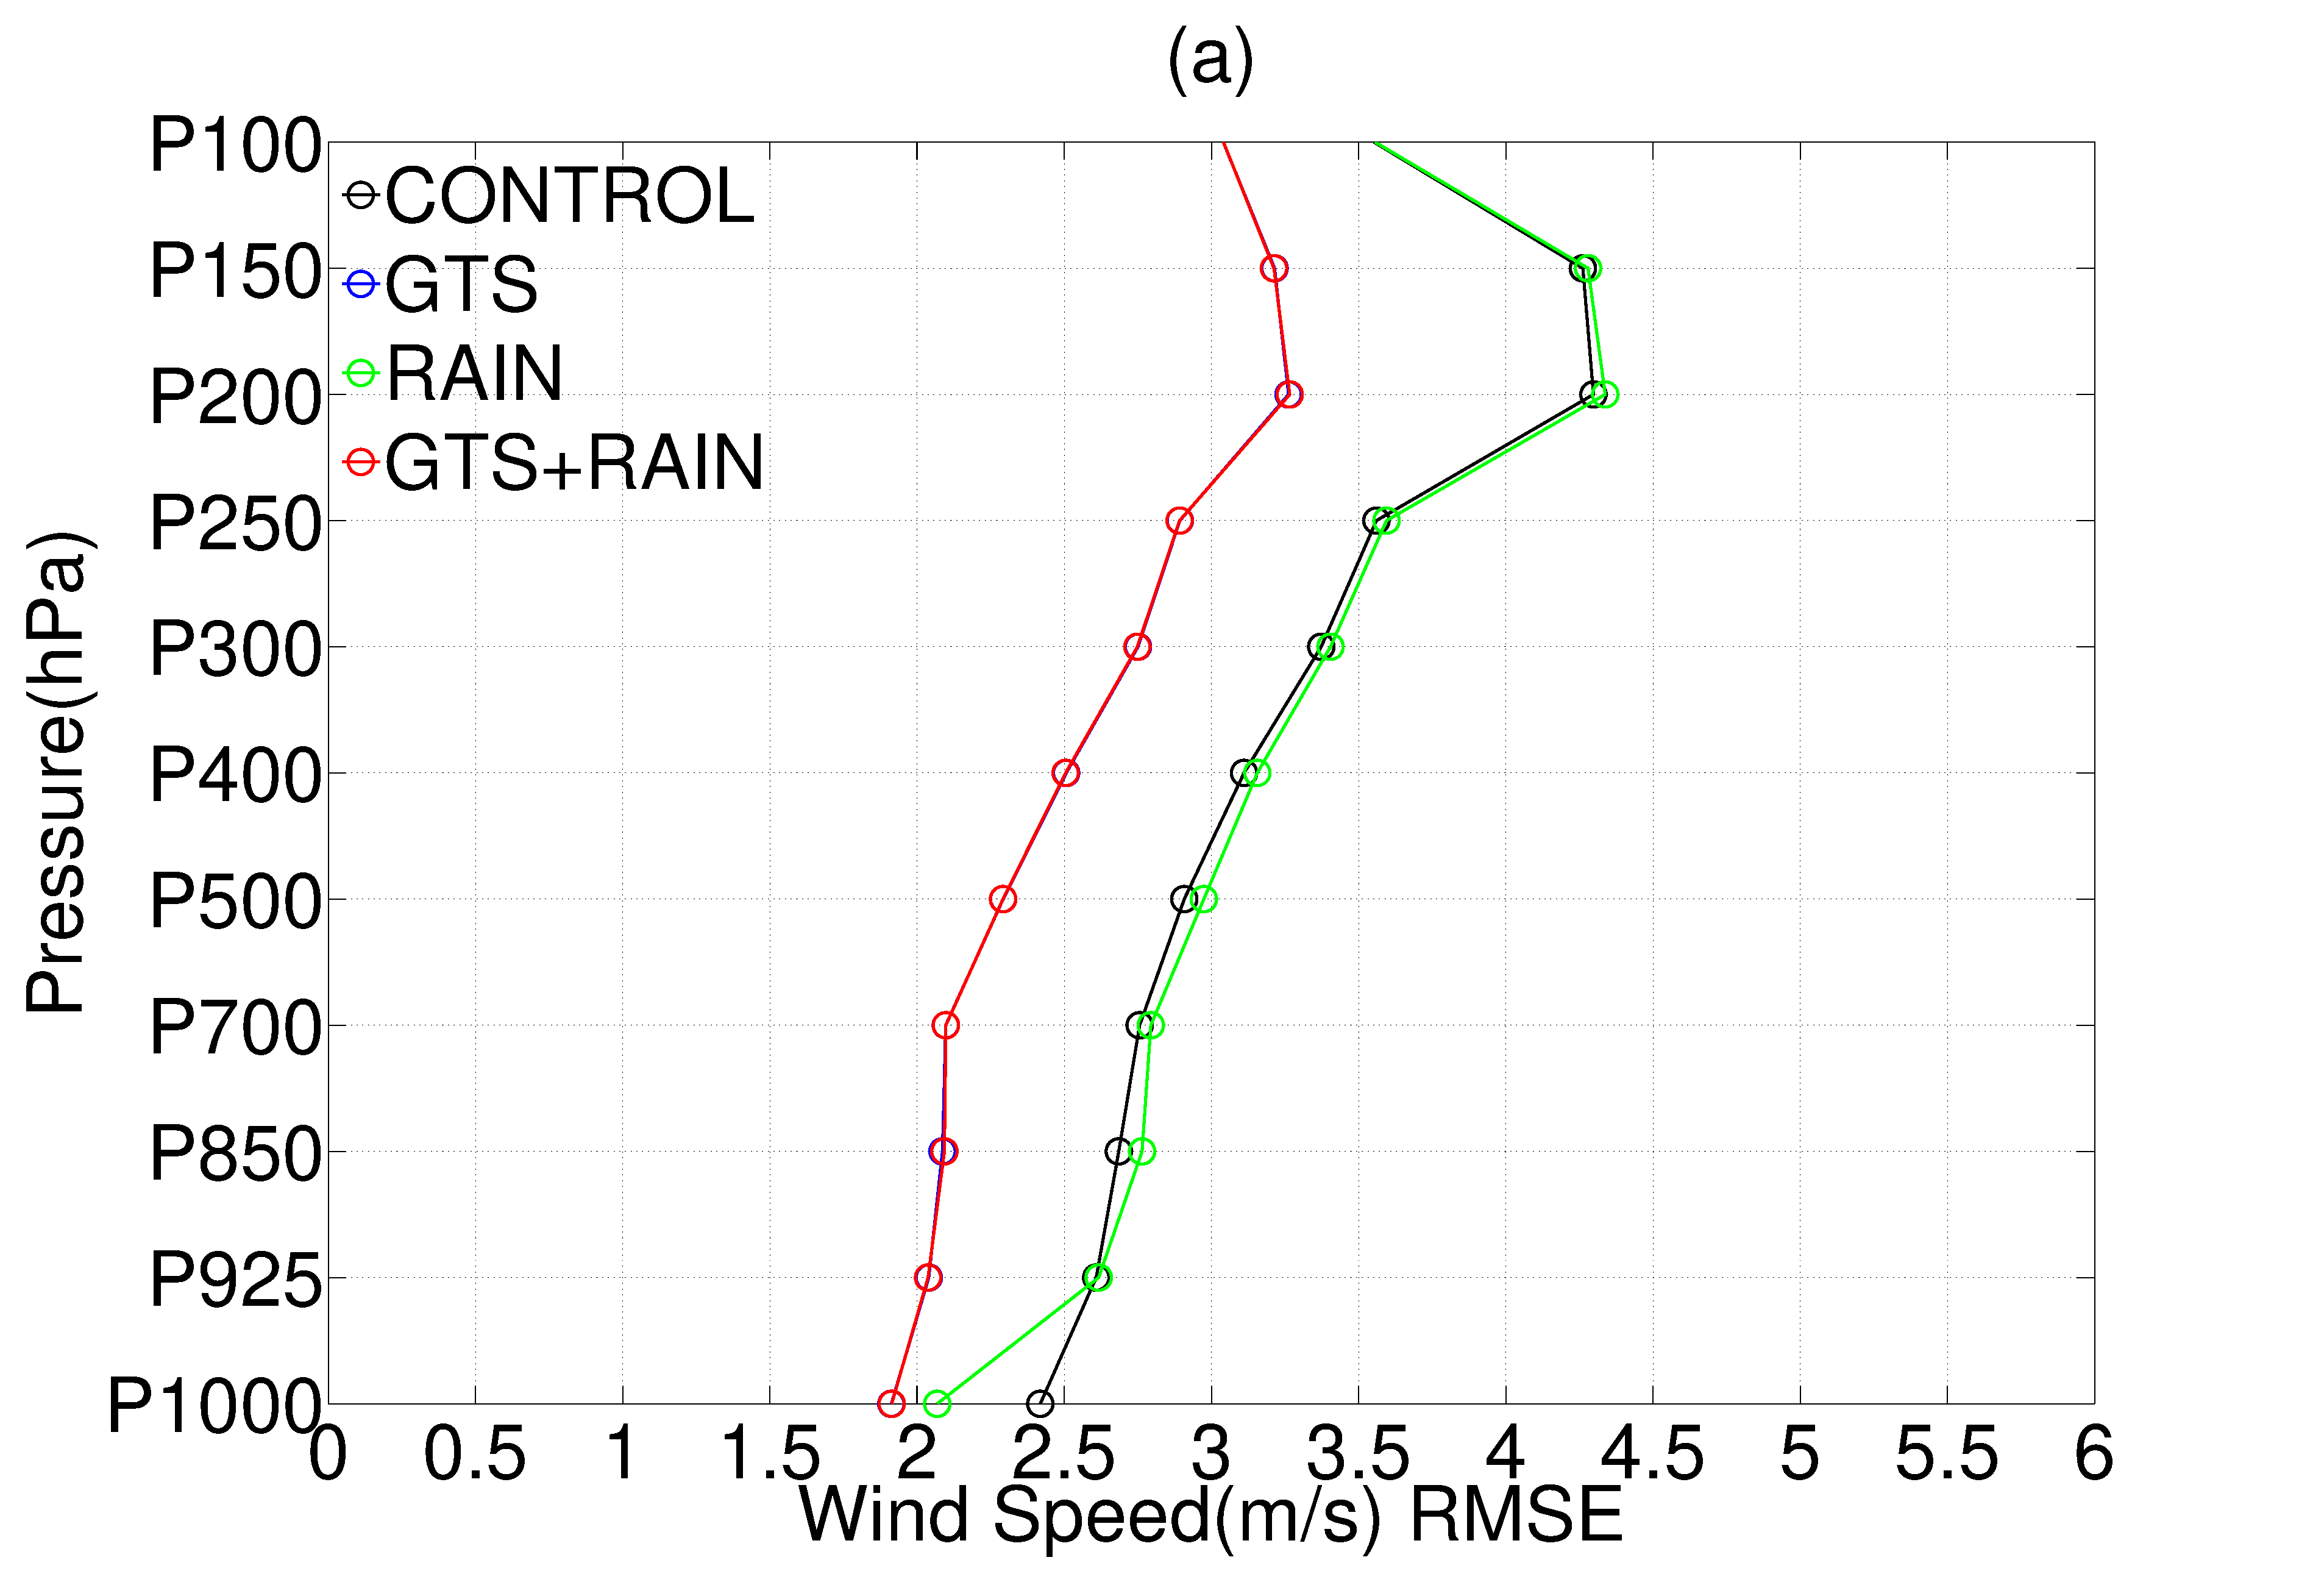
\includegraphics[width=0.45\linewidth]{./figures/wind_00.eps}

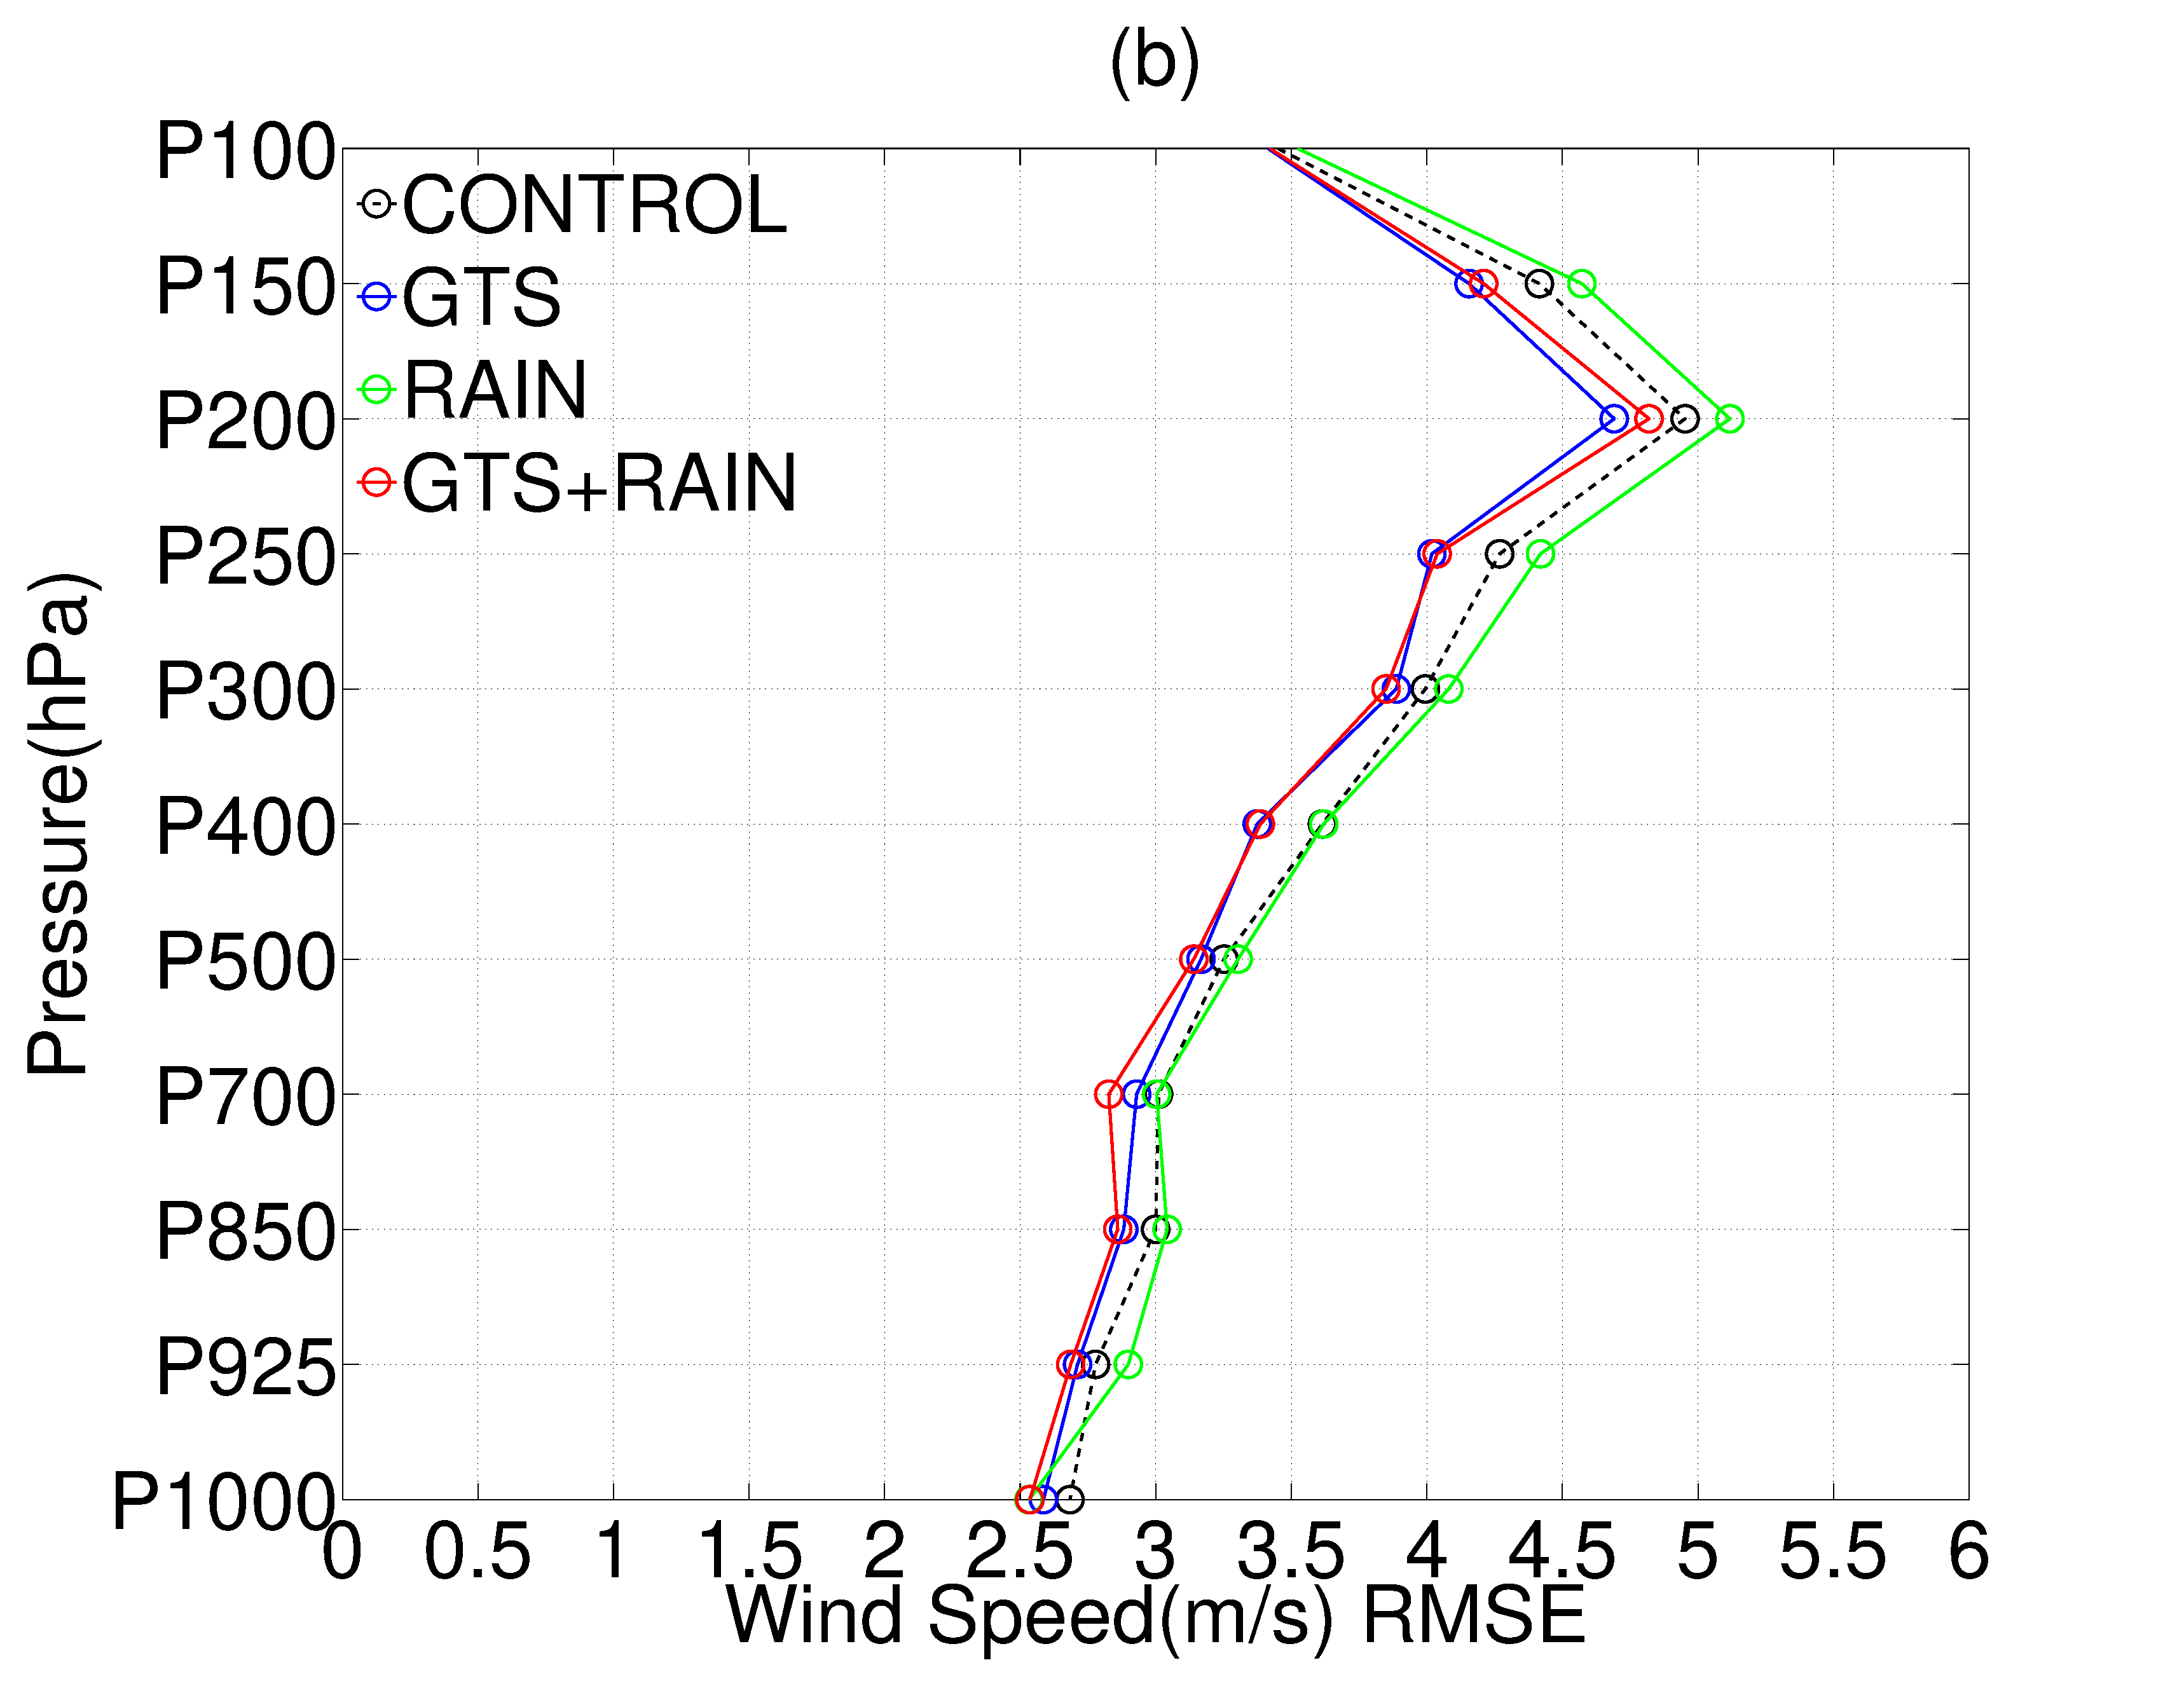
\includegraphics[width=0.45\linewidth]{./figures/wind_12.eps}

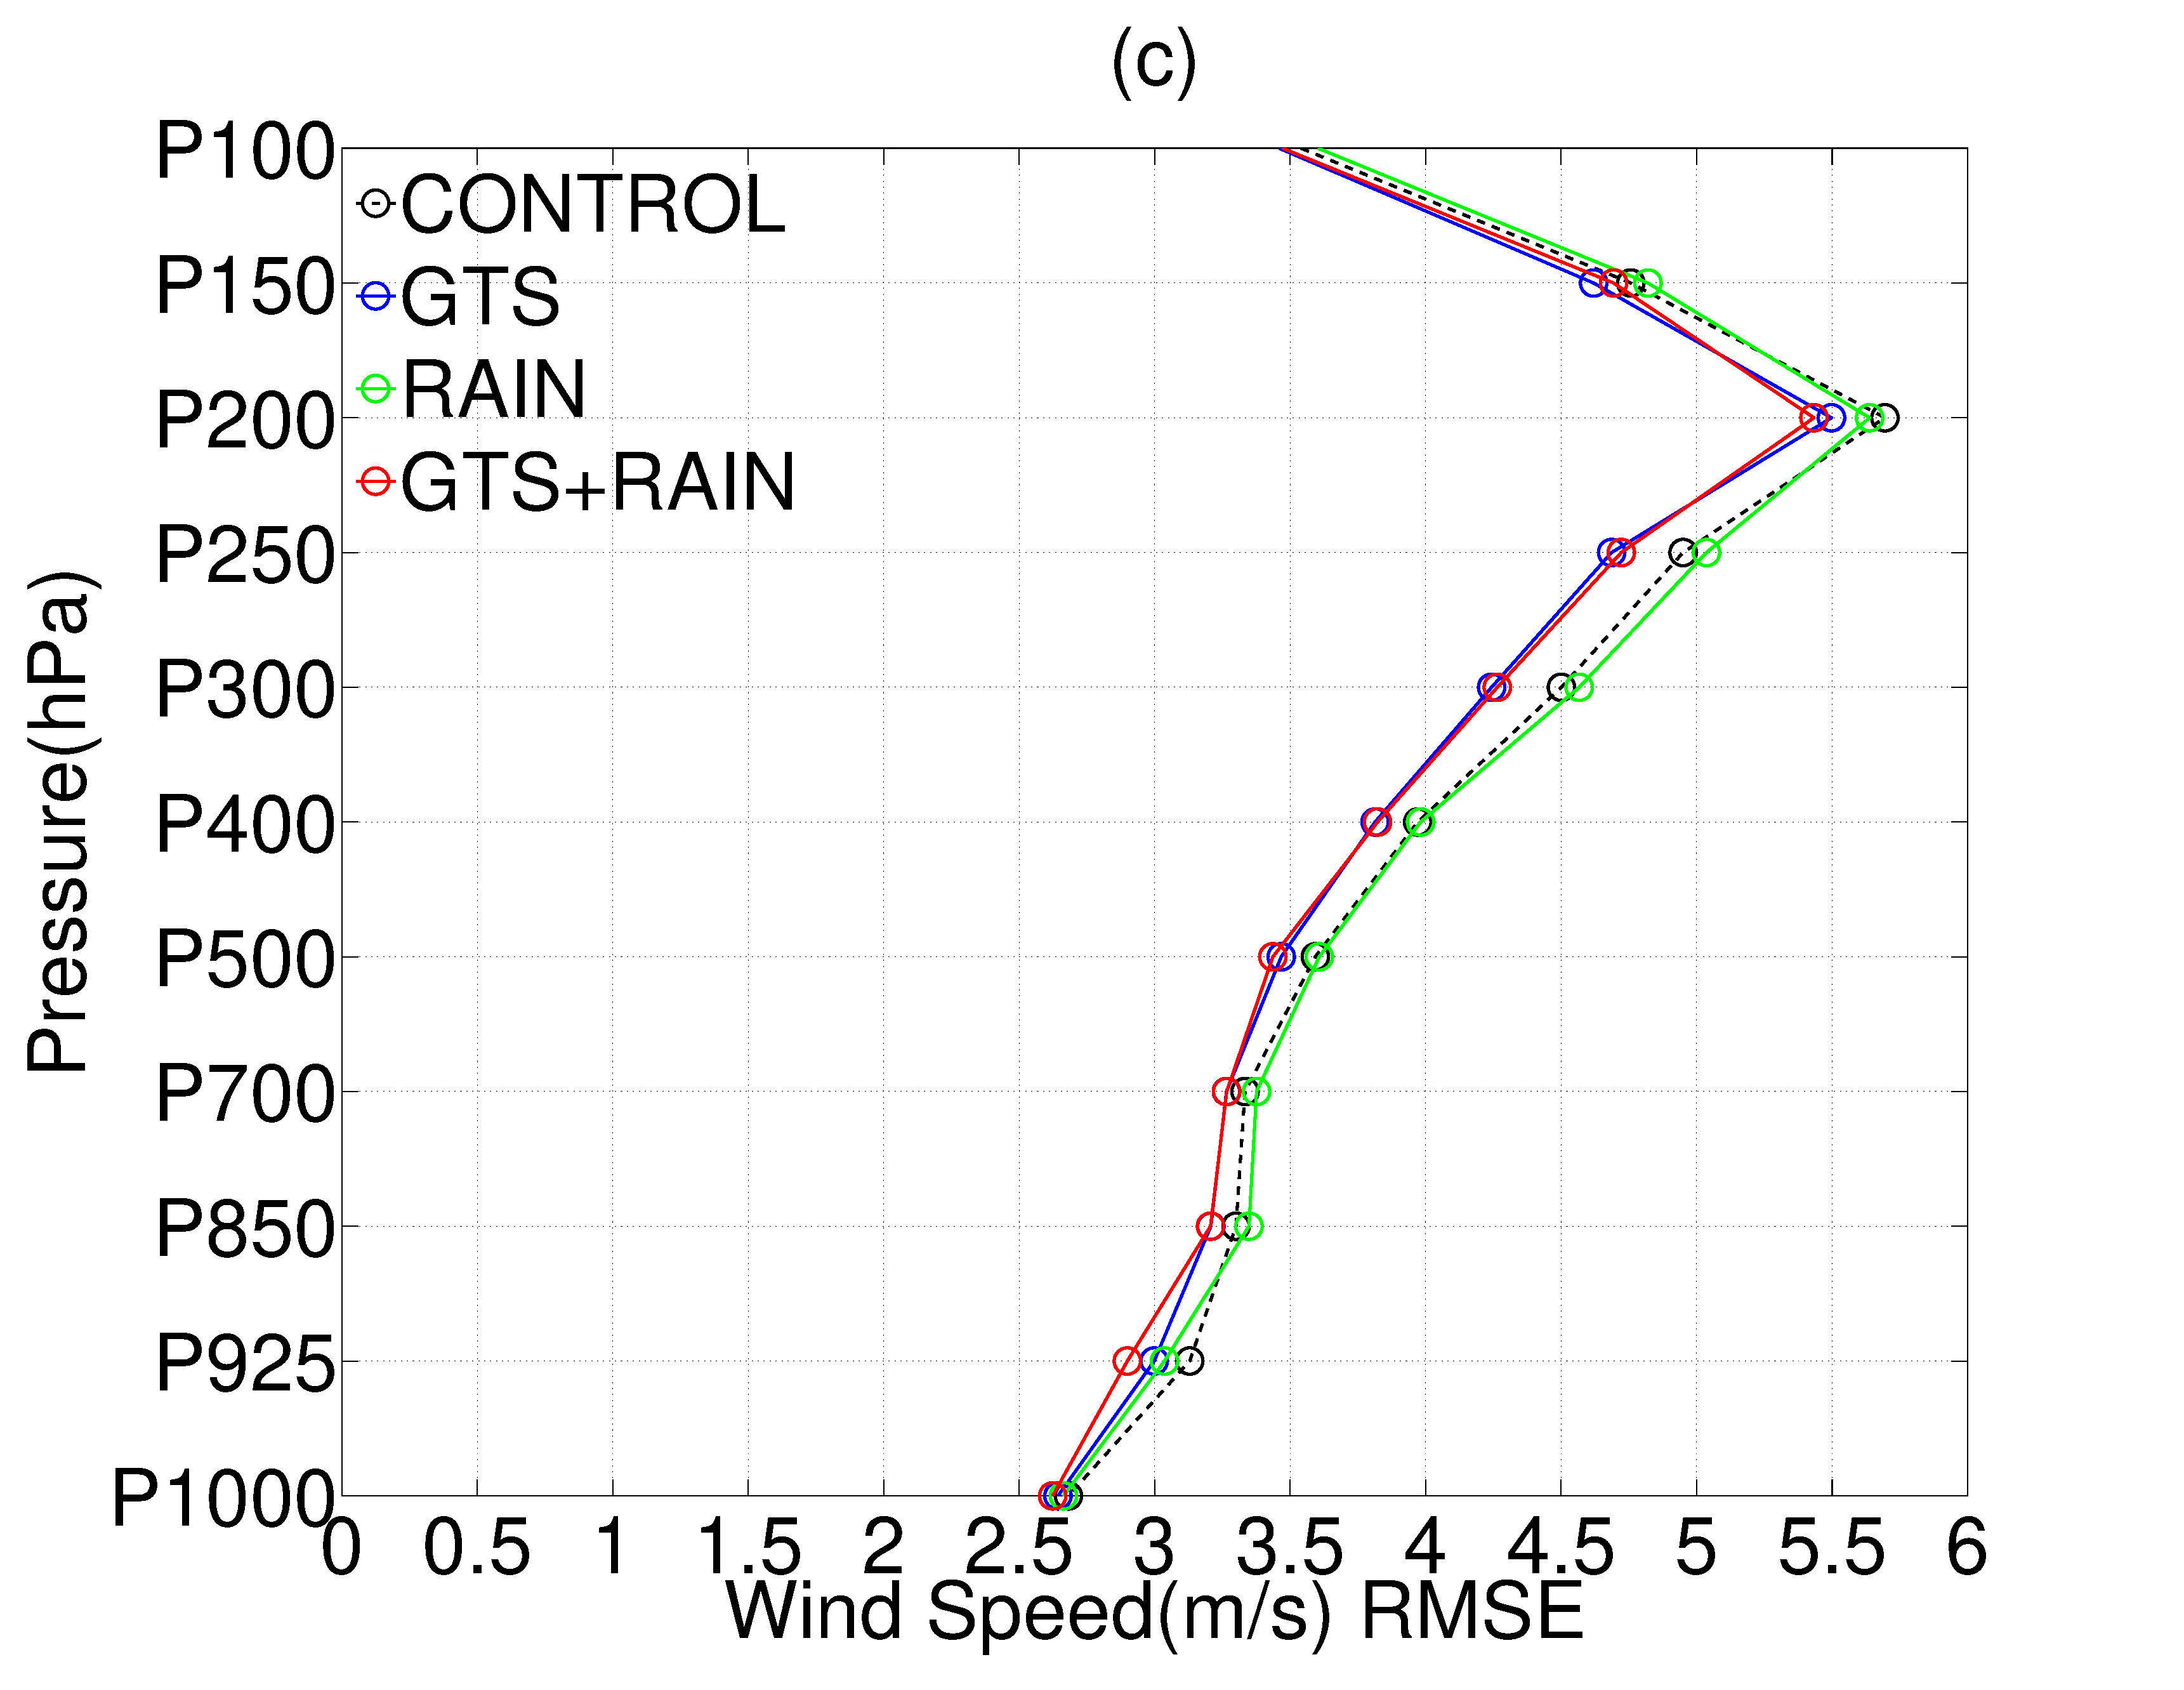
\includegraphics[width=0.45\linewidth]{./figures/wind_24.eps}
\caption{Vertical profile of wind speed RMSE for experiments CONTROL, GTS, RAIN and GTS+RAIN for analysis (a), 12-h forecast(b) and 24-h forecast(c) aggregated over 10-day period of cases verified against upper air sounding data.}\label{u_00}
\end{figure}


\newpage
\begin{figure}
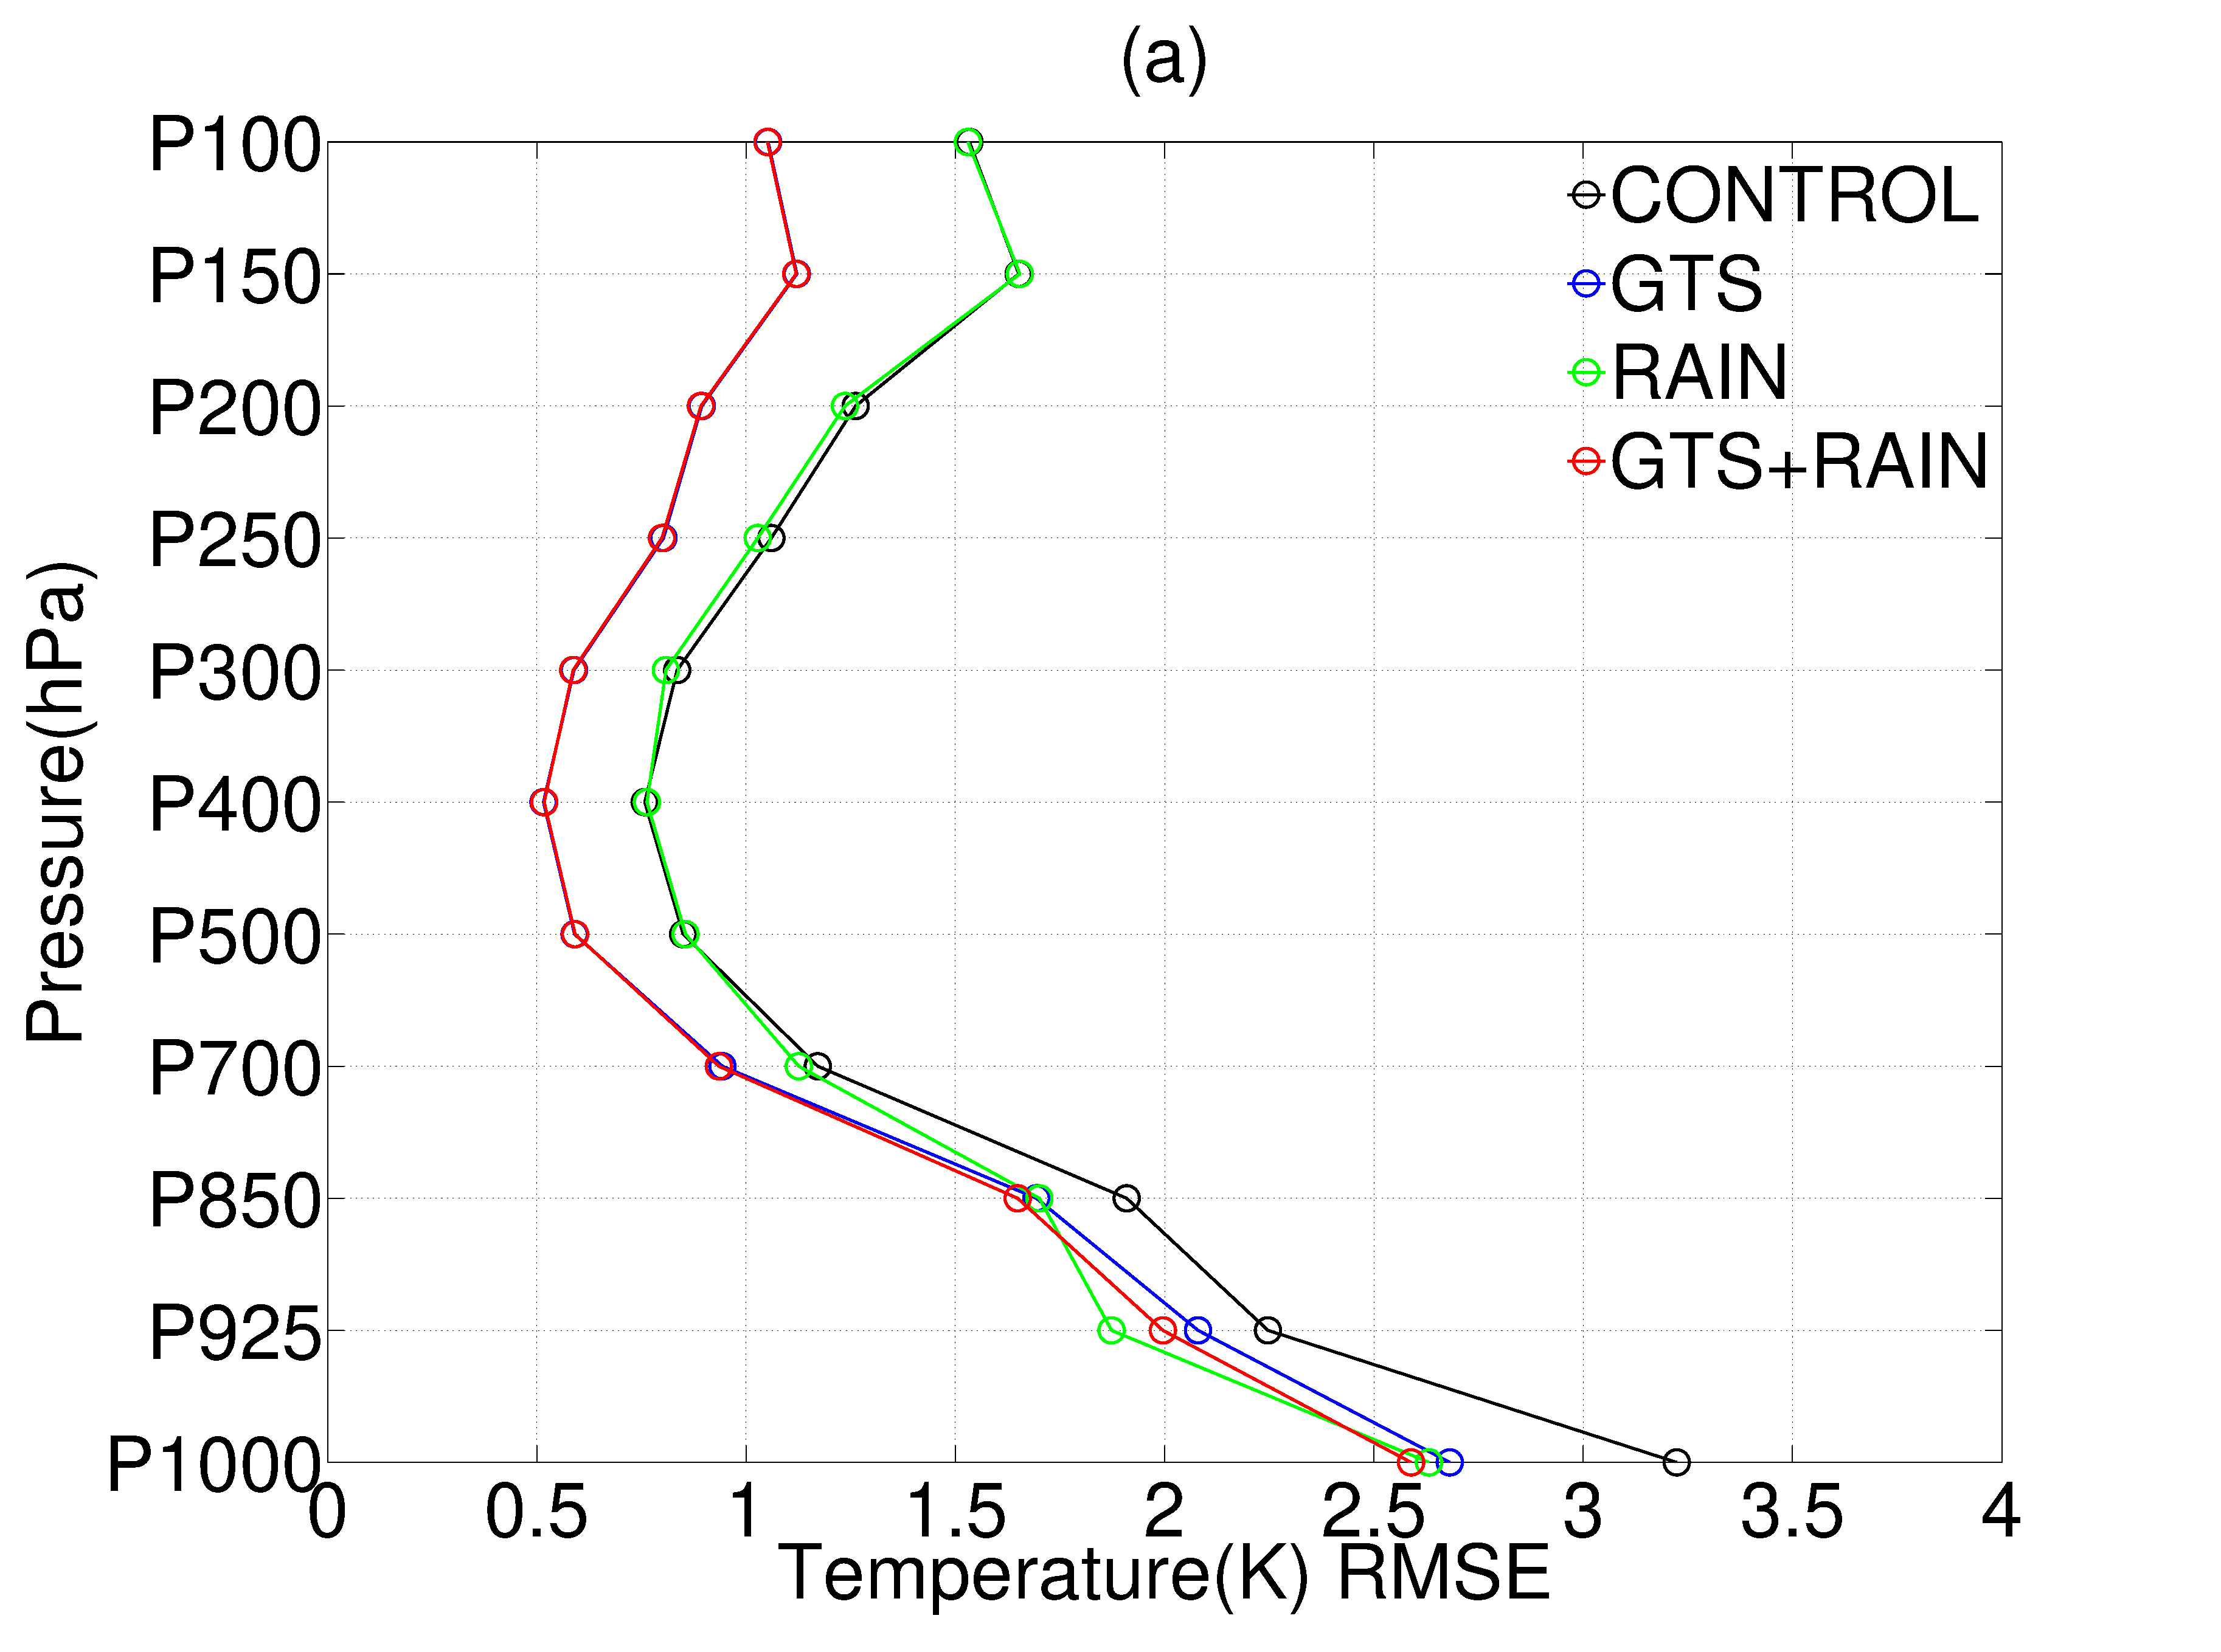
\includegraphics[width=0.5\linewidth]{./figures/tmp_00.eps}

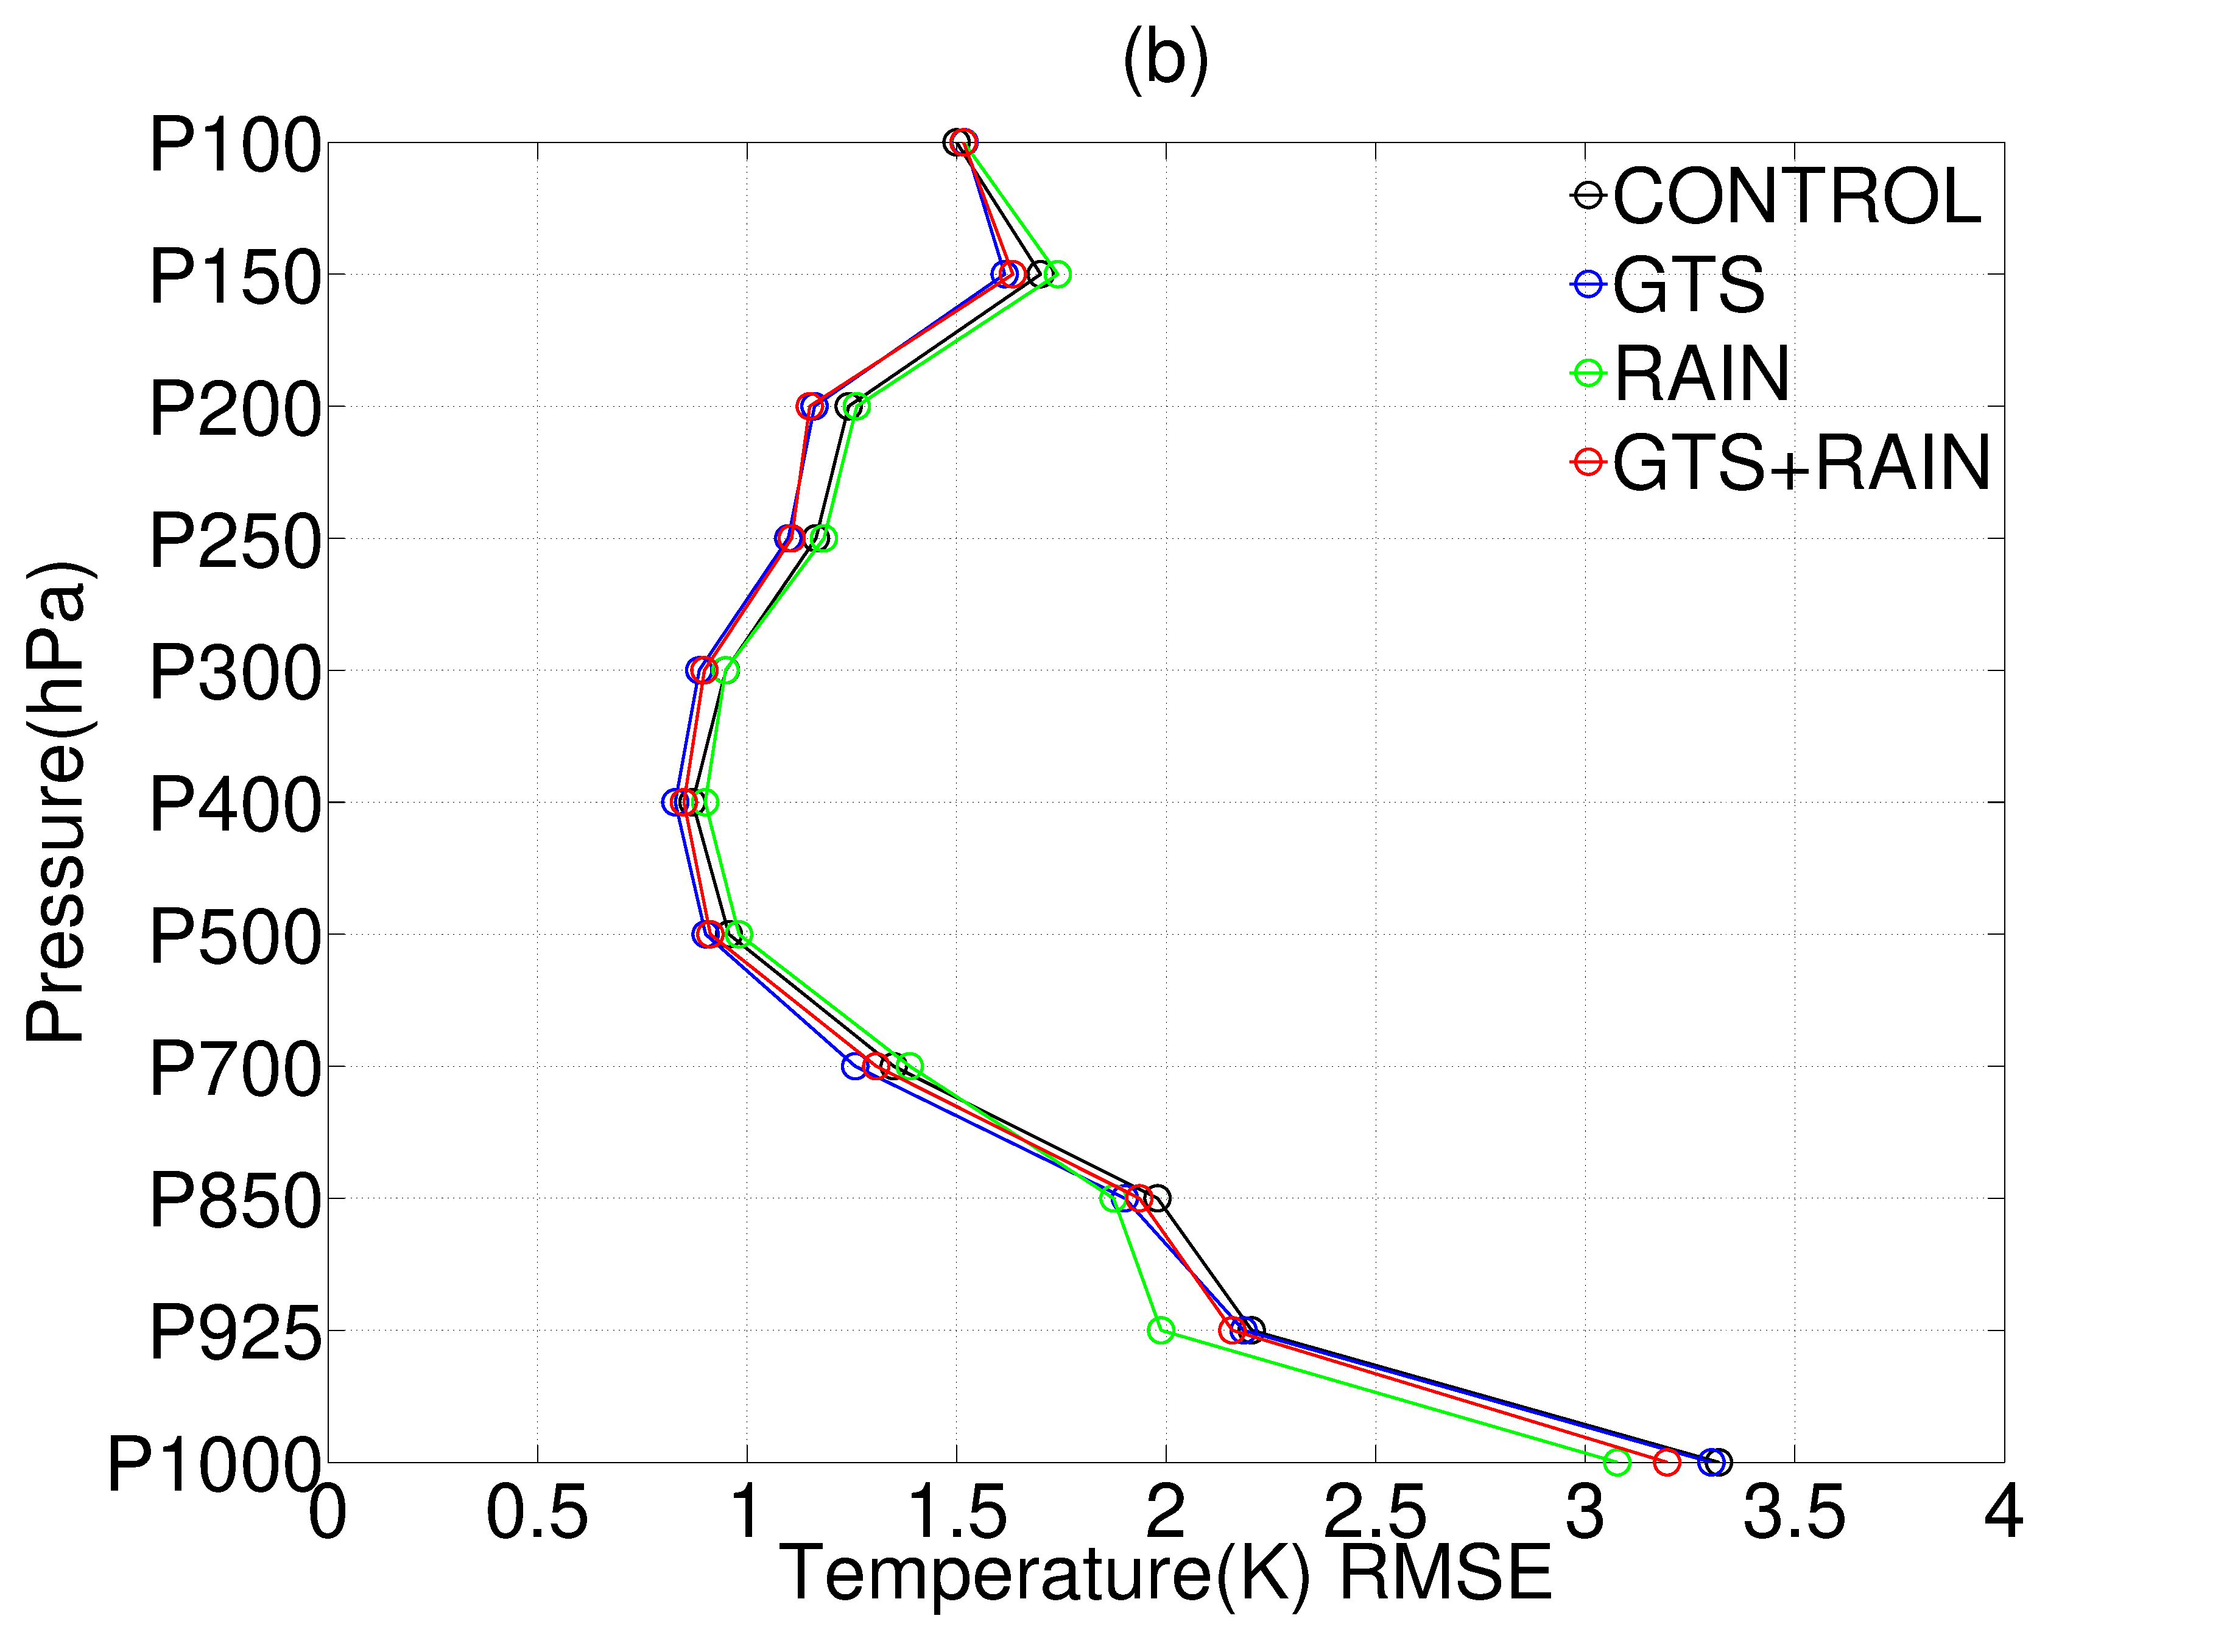
\includegraphics[width=0.5\linewidth]{./figures/tmp_12.eps}

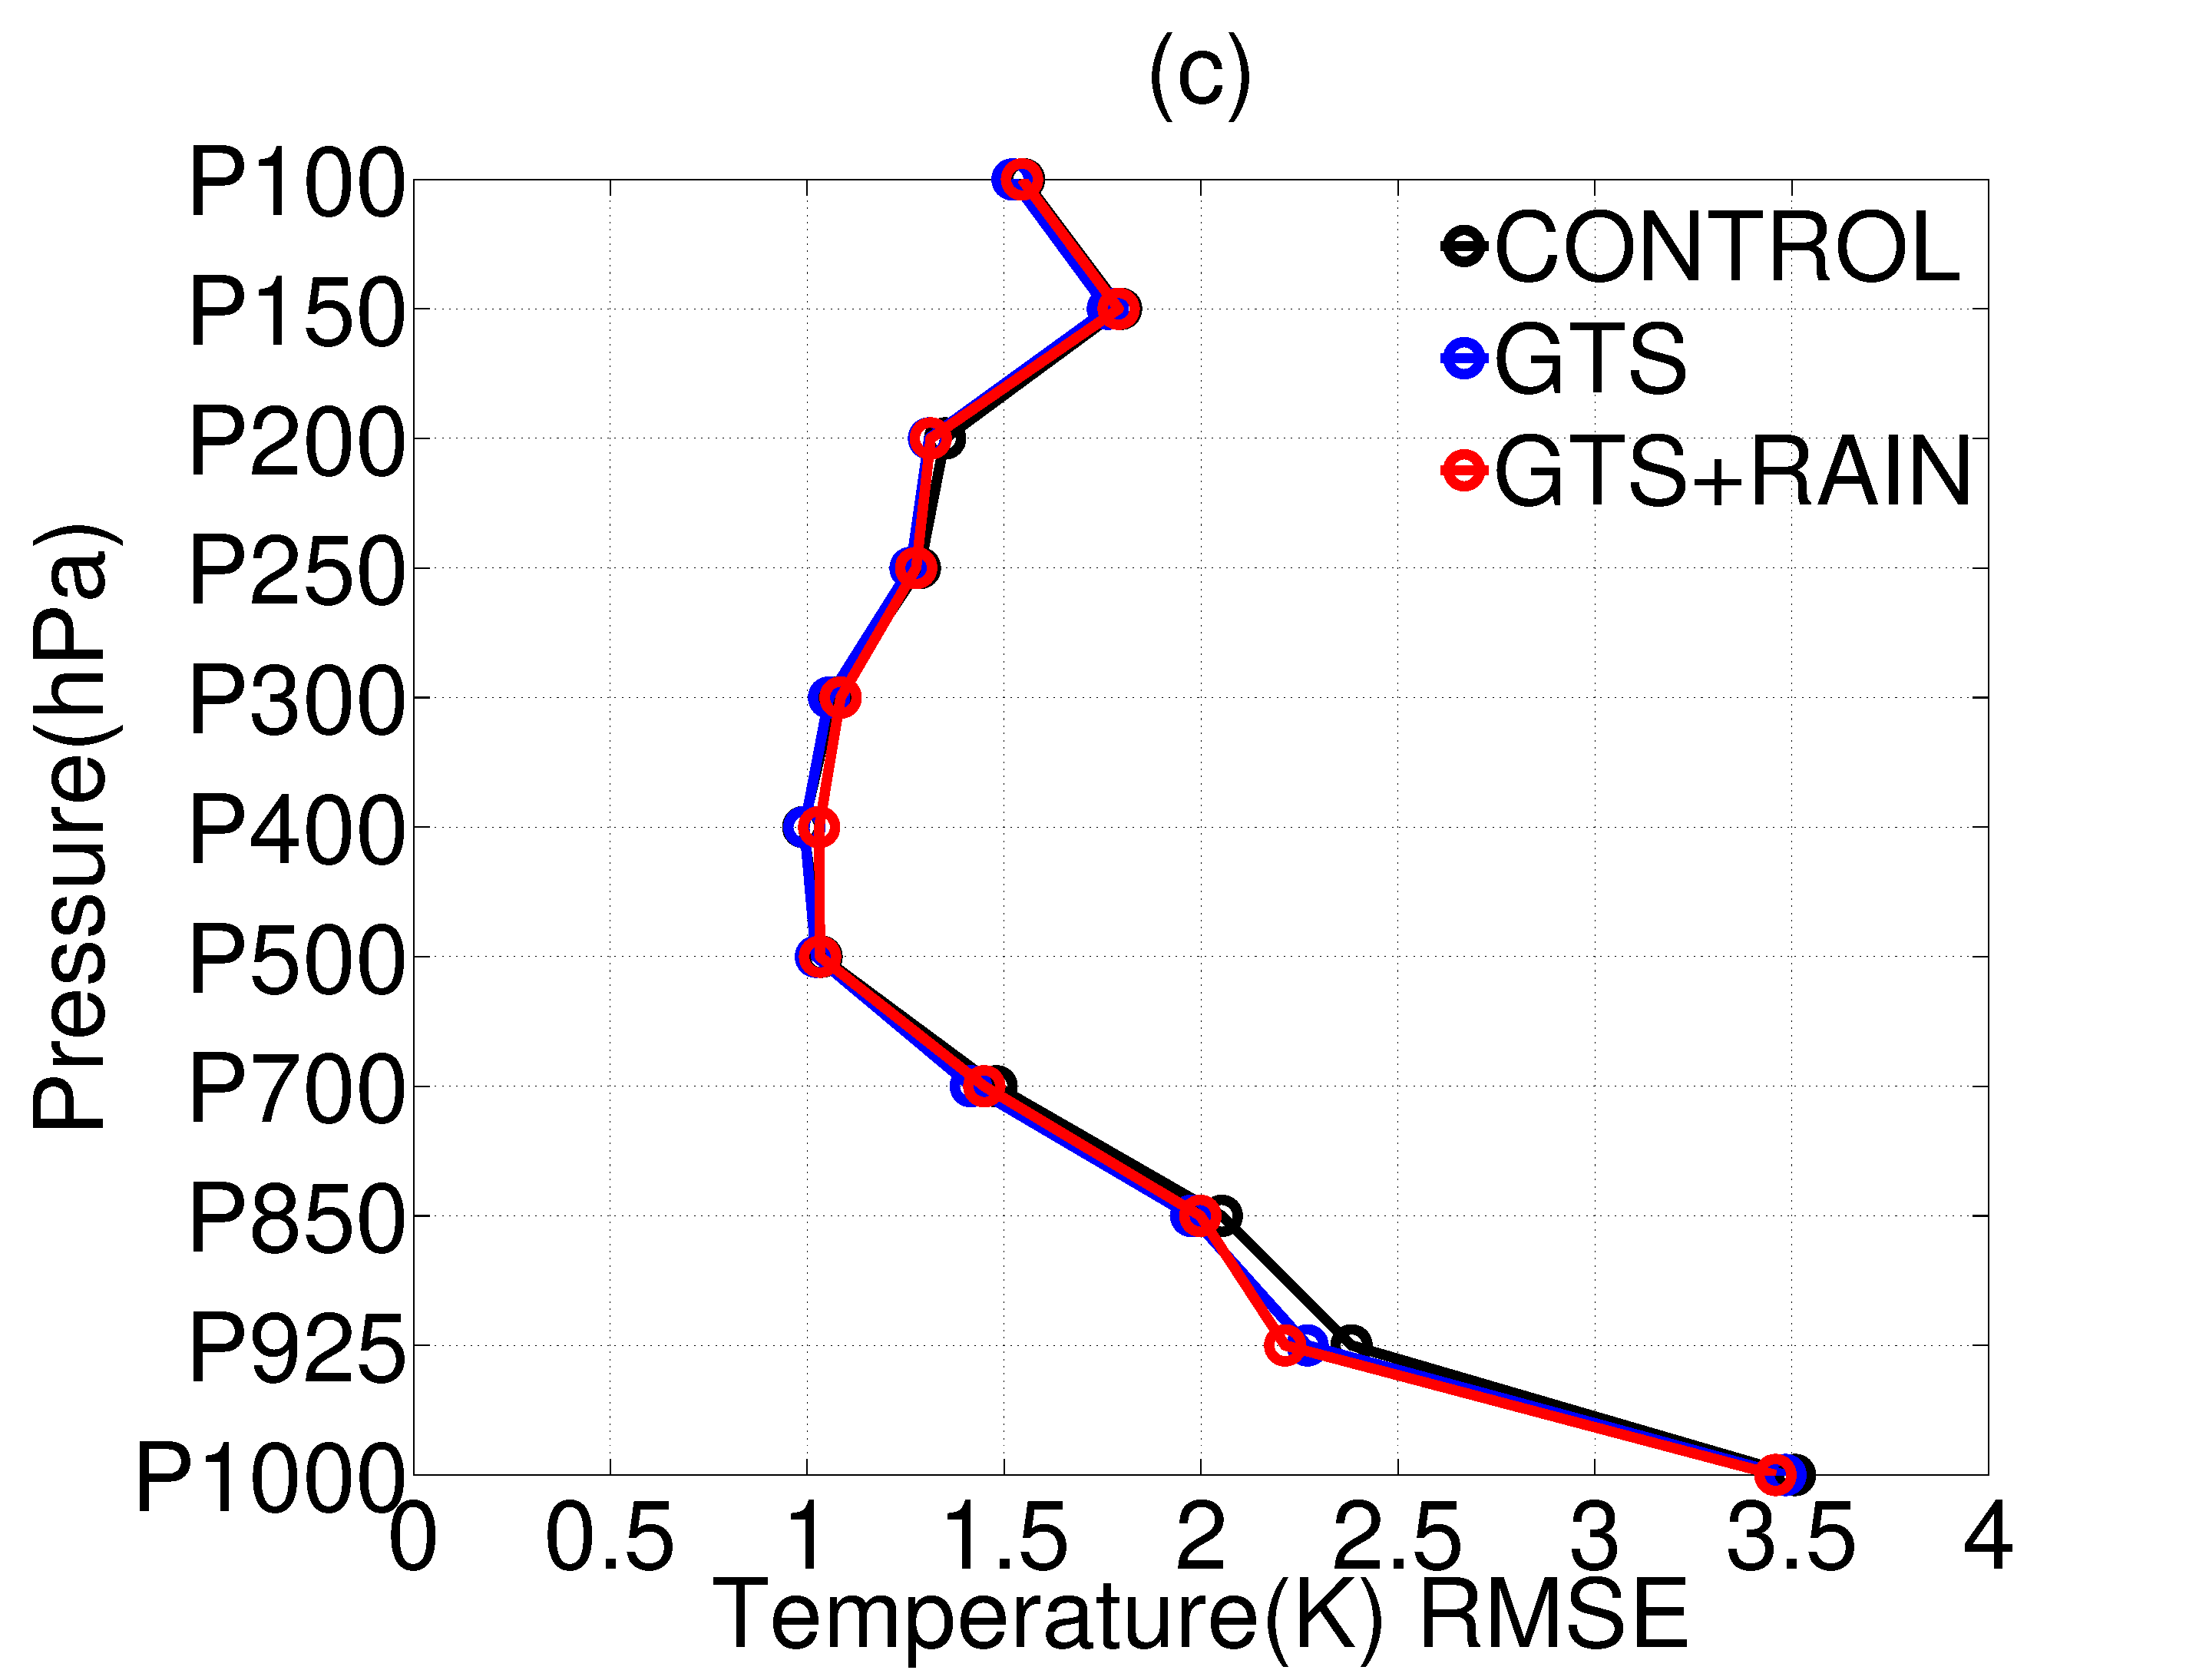
\includegraphics[width=0.5\linewidth]{./figures/tmp_24.eps}
\caption{Same as Figure 1 but for temperature. }\label{tmp_00}
\end{figure}

\newpage
\begin{figure}
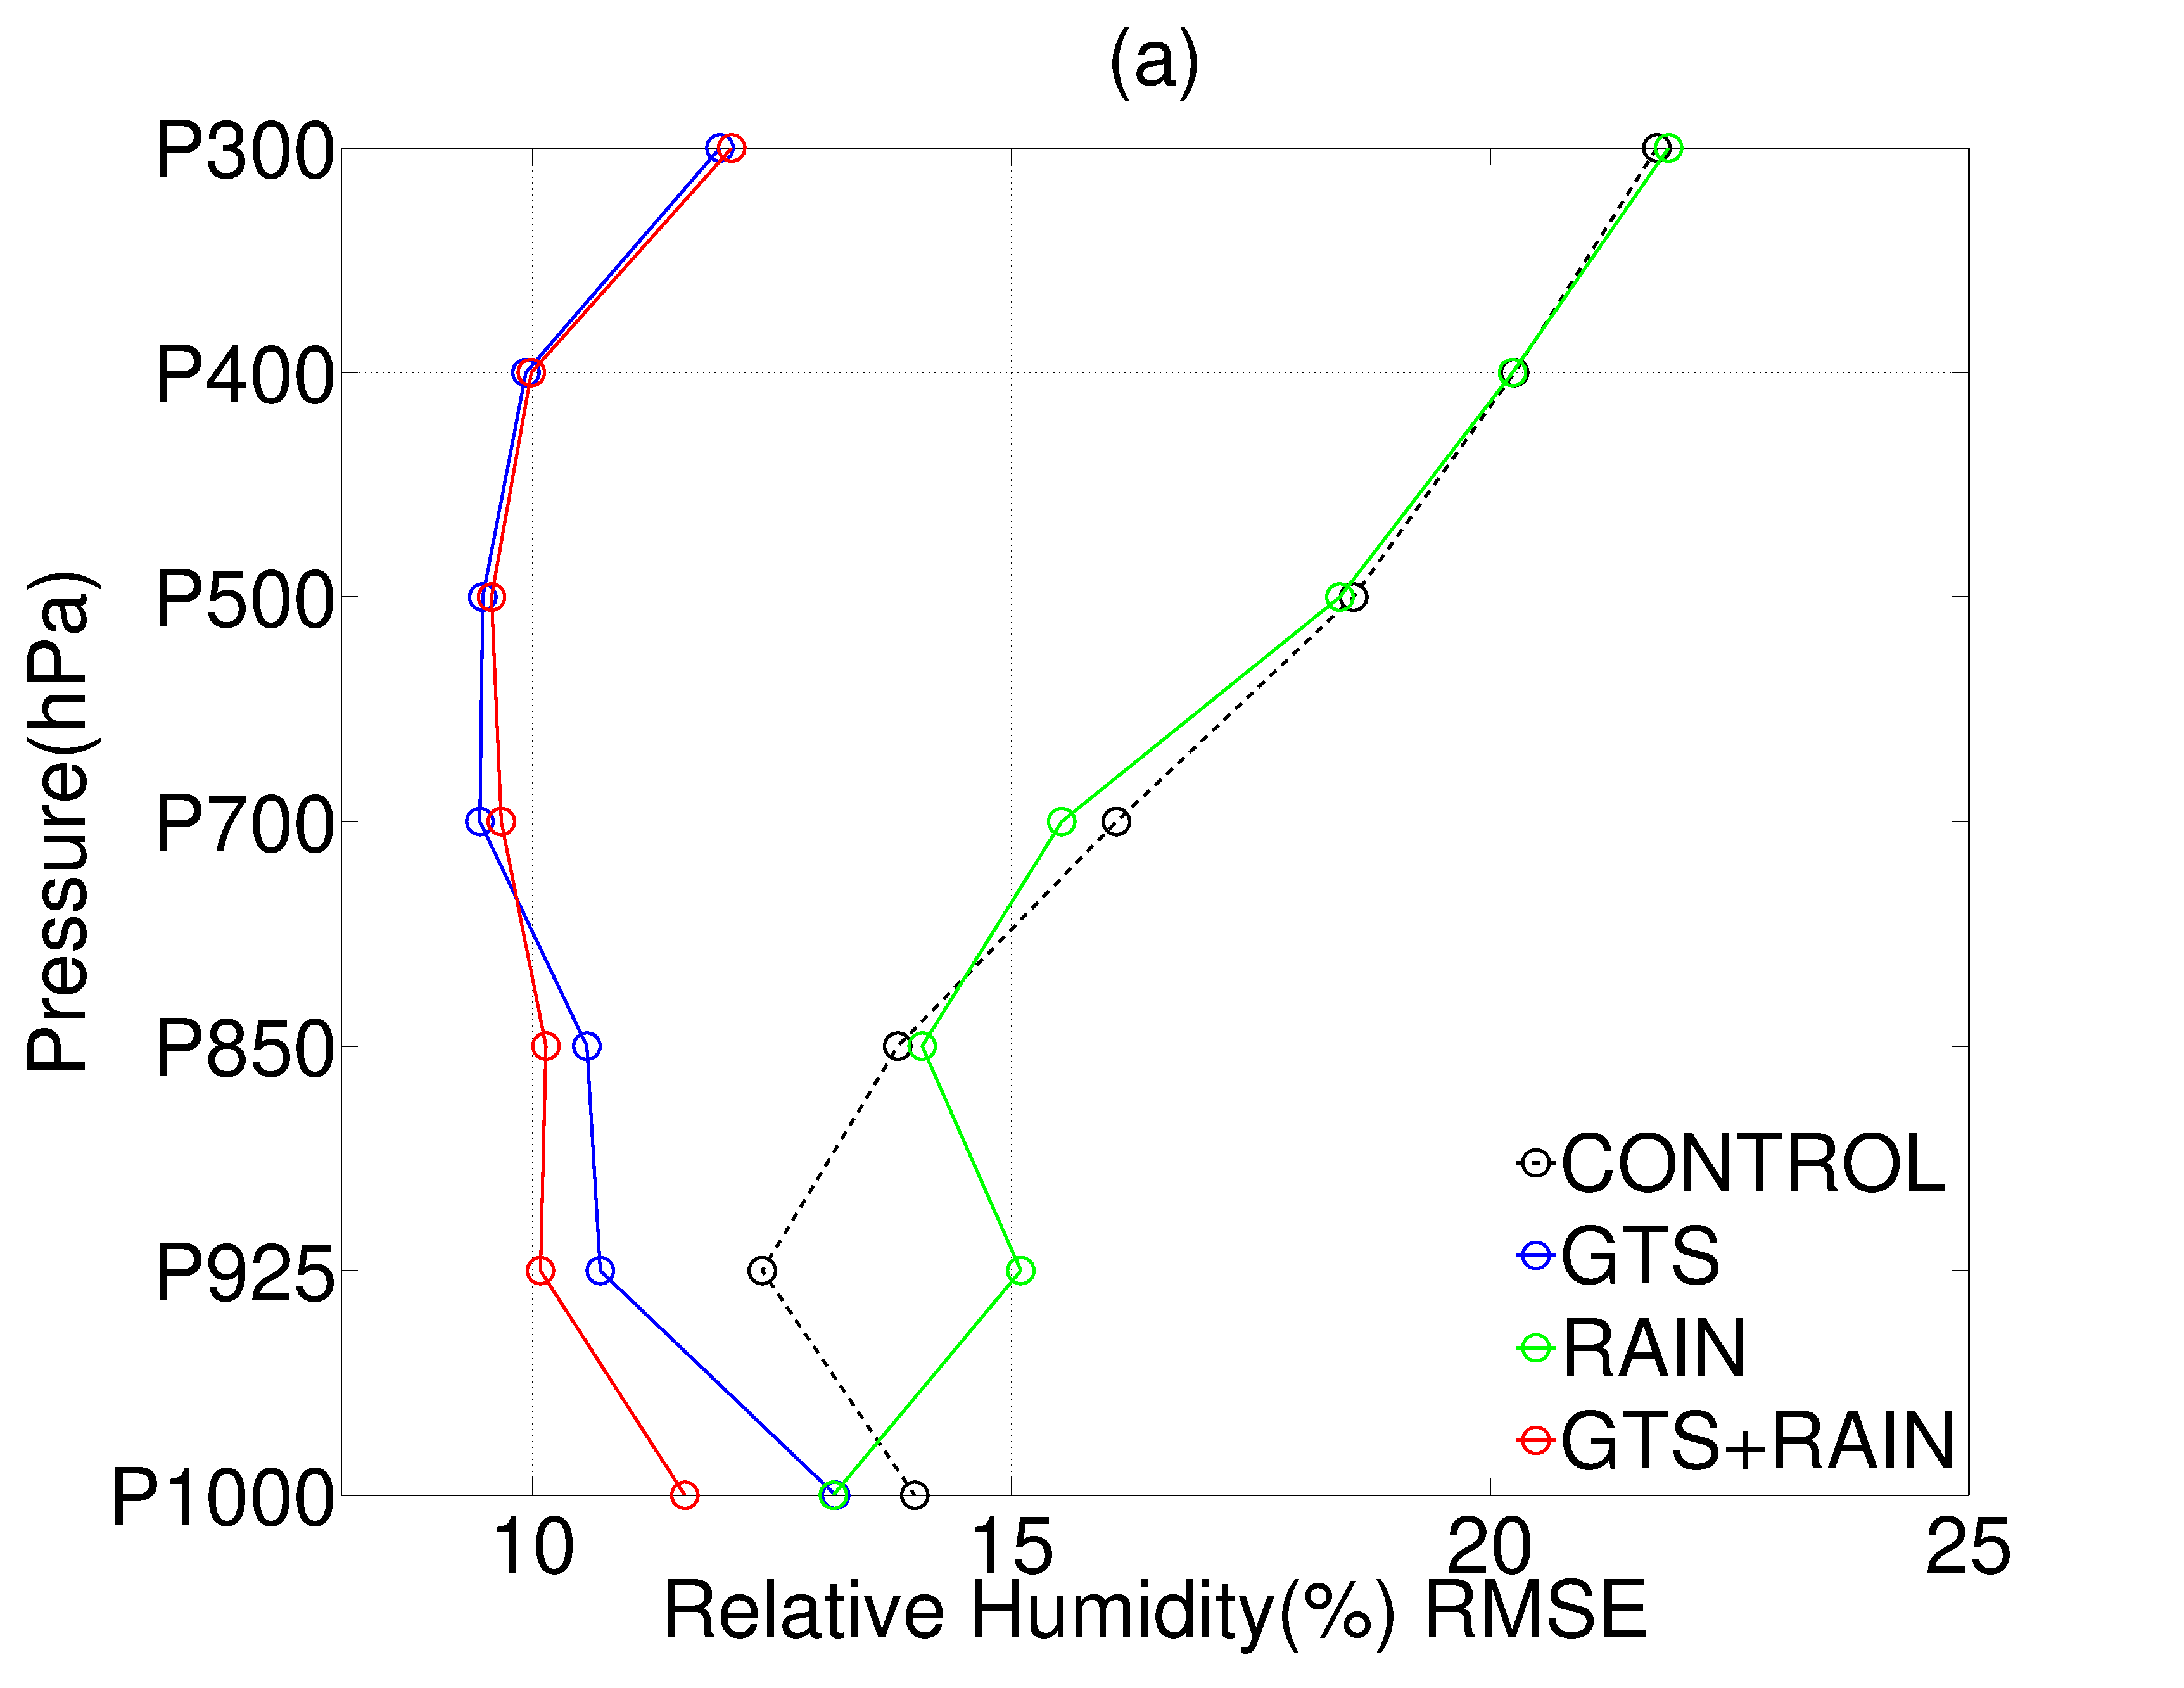
\includegraphics[width=0.5\linewidth]{./figures/rh_00.eps}

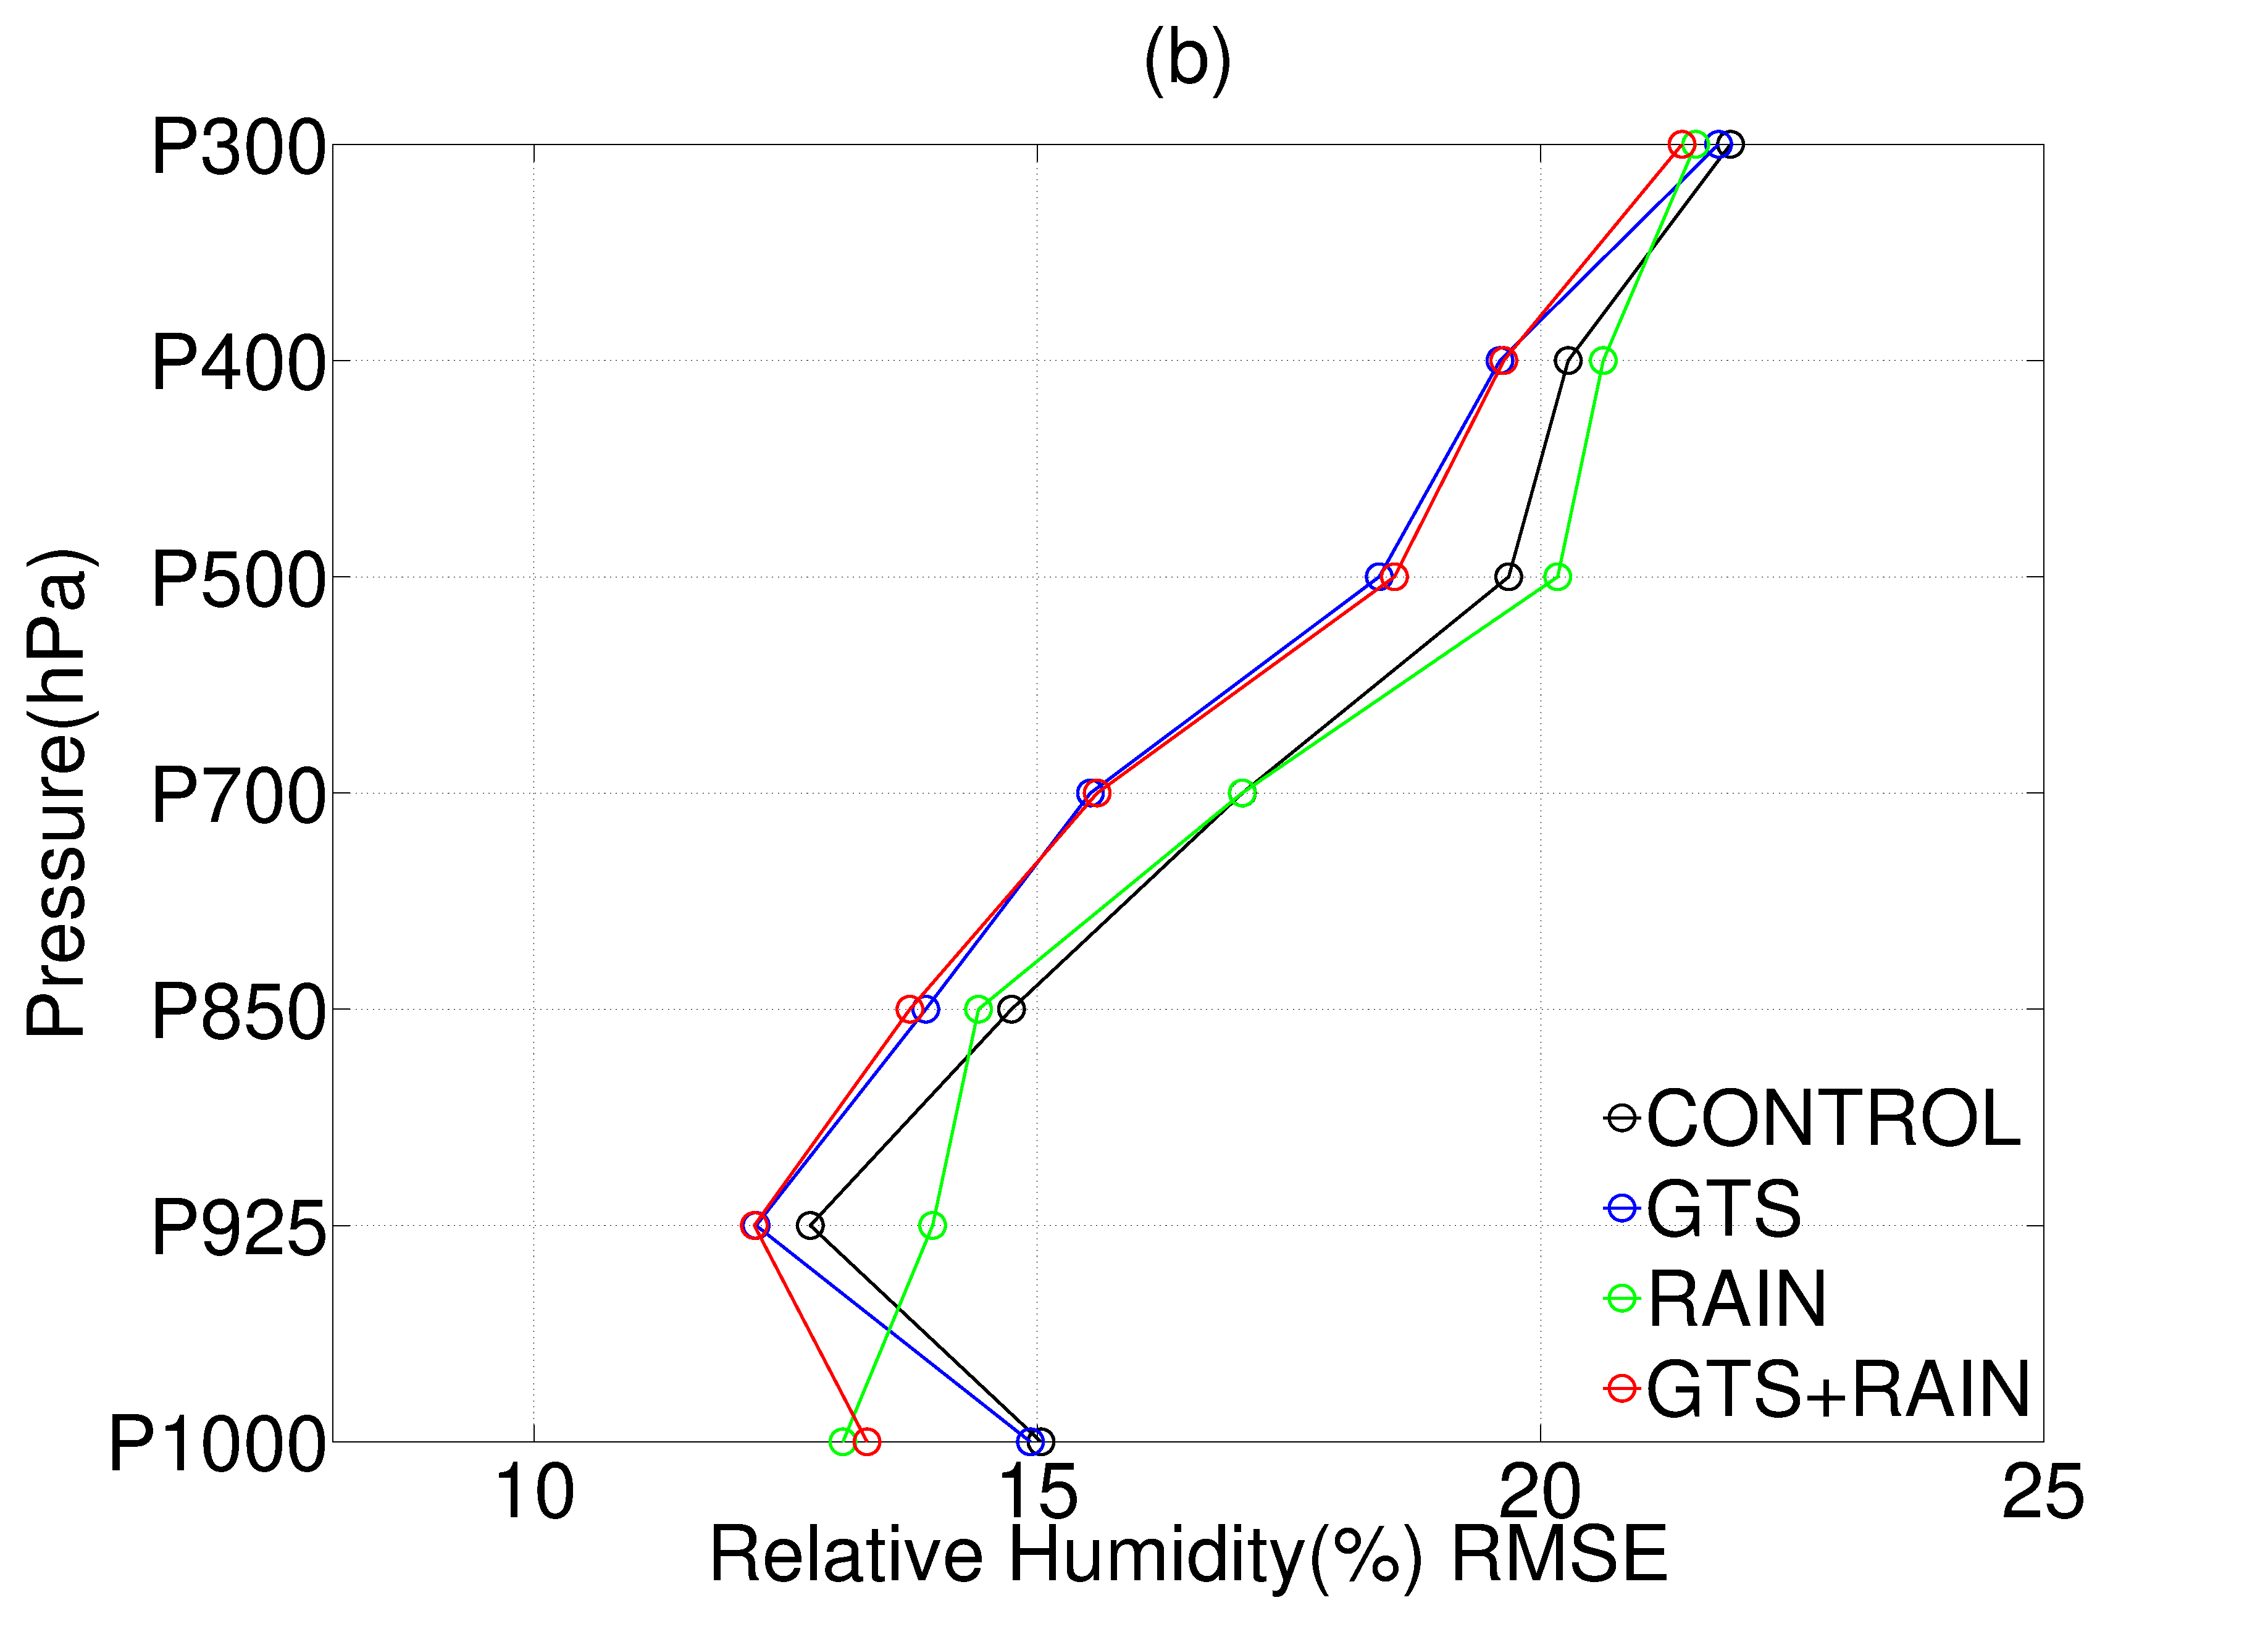
\includegraphics[width=0.5\linewidth]{./figures/rh_12.eps}

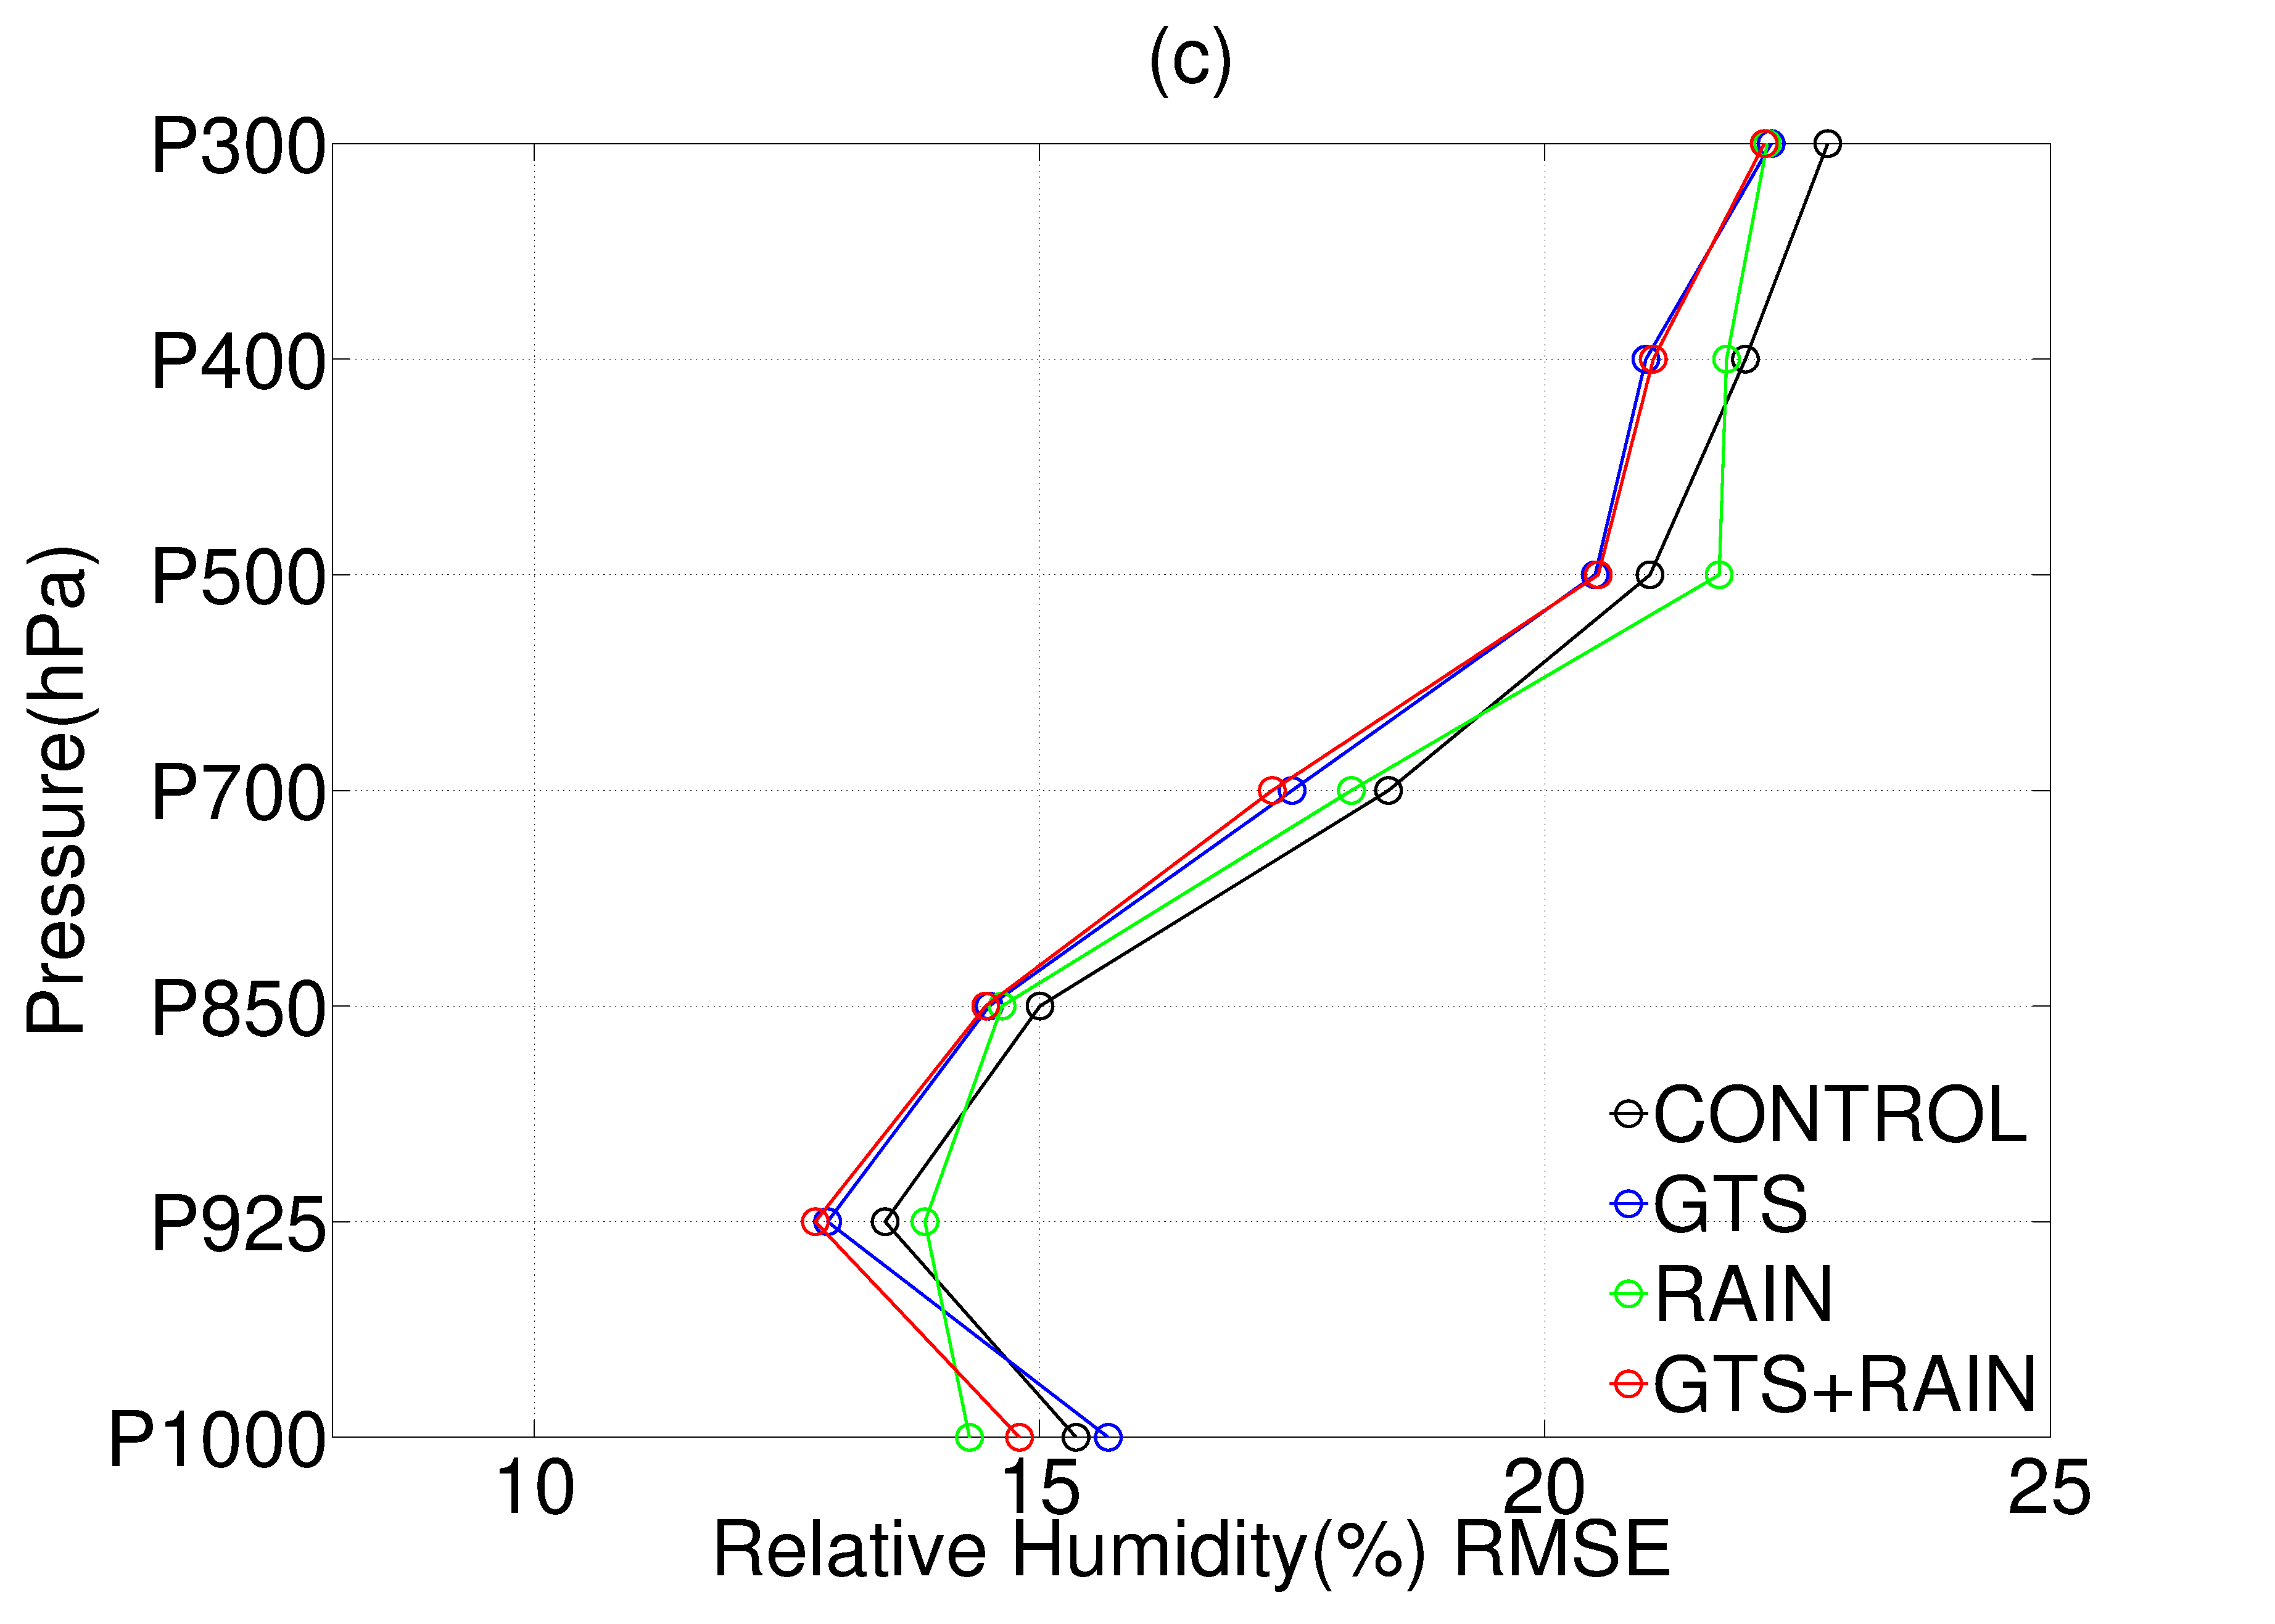
\includegraphics[width=0.5\linewidth]{./figures/rh_24.eps}
\caption{Same as Figure 1 but for relative humidity.}\label{rh_00}
\end{figure}

\newpage
\begin{figure}
%\includegraphics[width=0.5\linewidth]{./figures/gss_6h_error.eps}
%\includegraphics[width=0.5\linewidth]{./figures/gss_12h_error.eps}
%\includegraphics[width=0.5\linewidth]{./figures/gss_18h_error.eps}
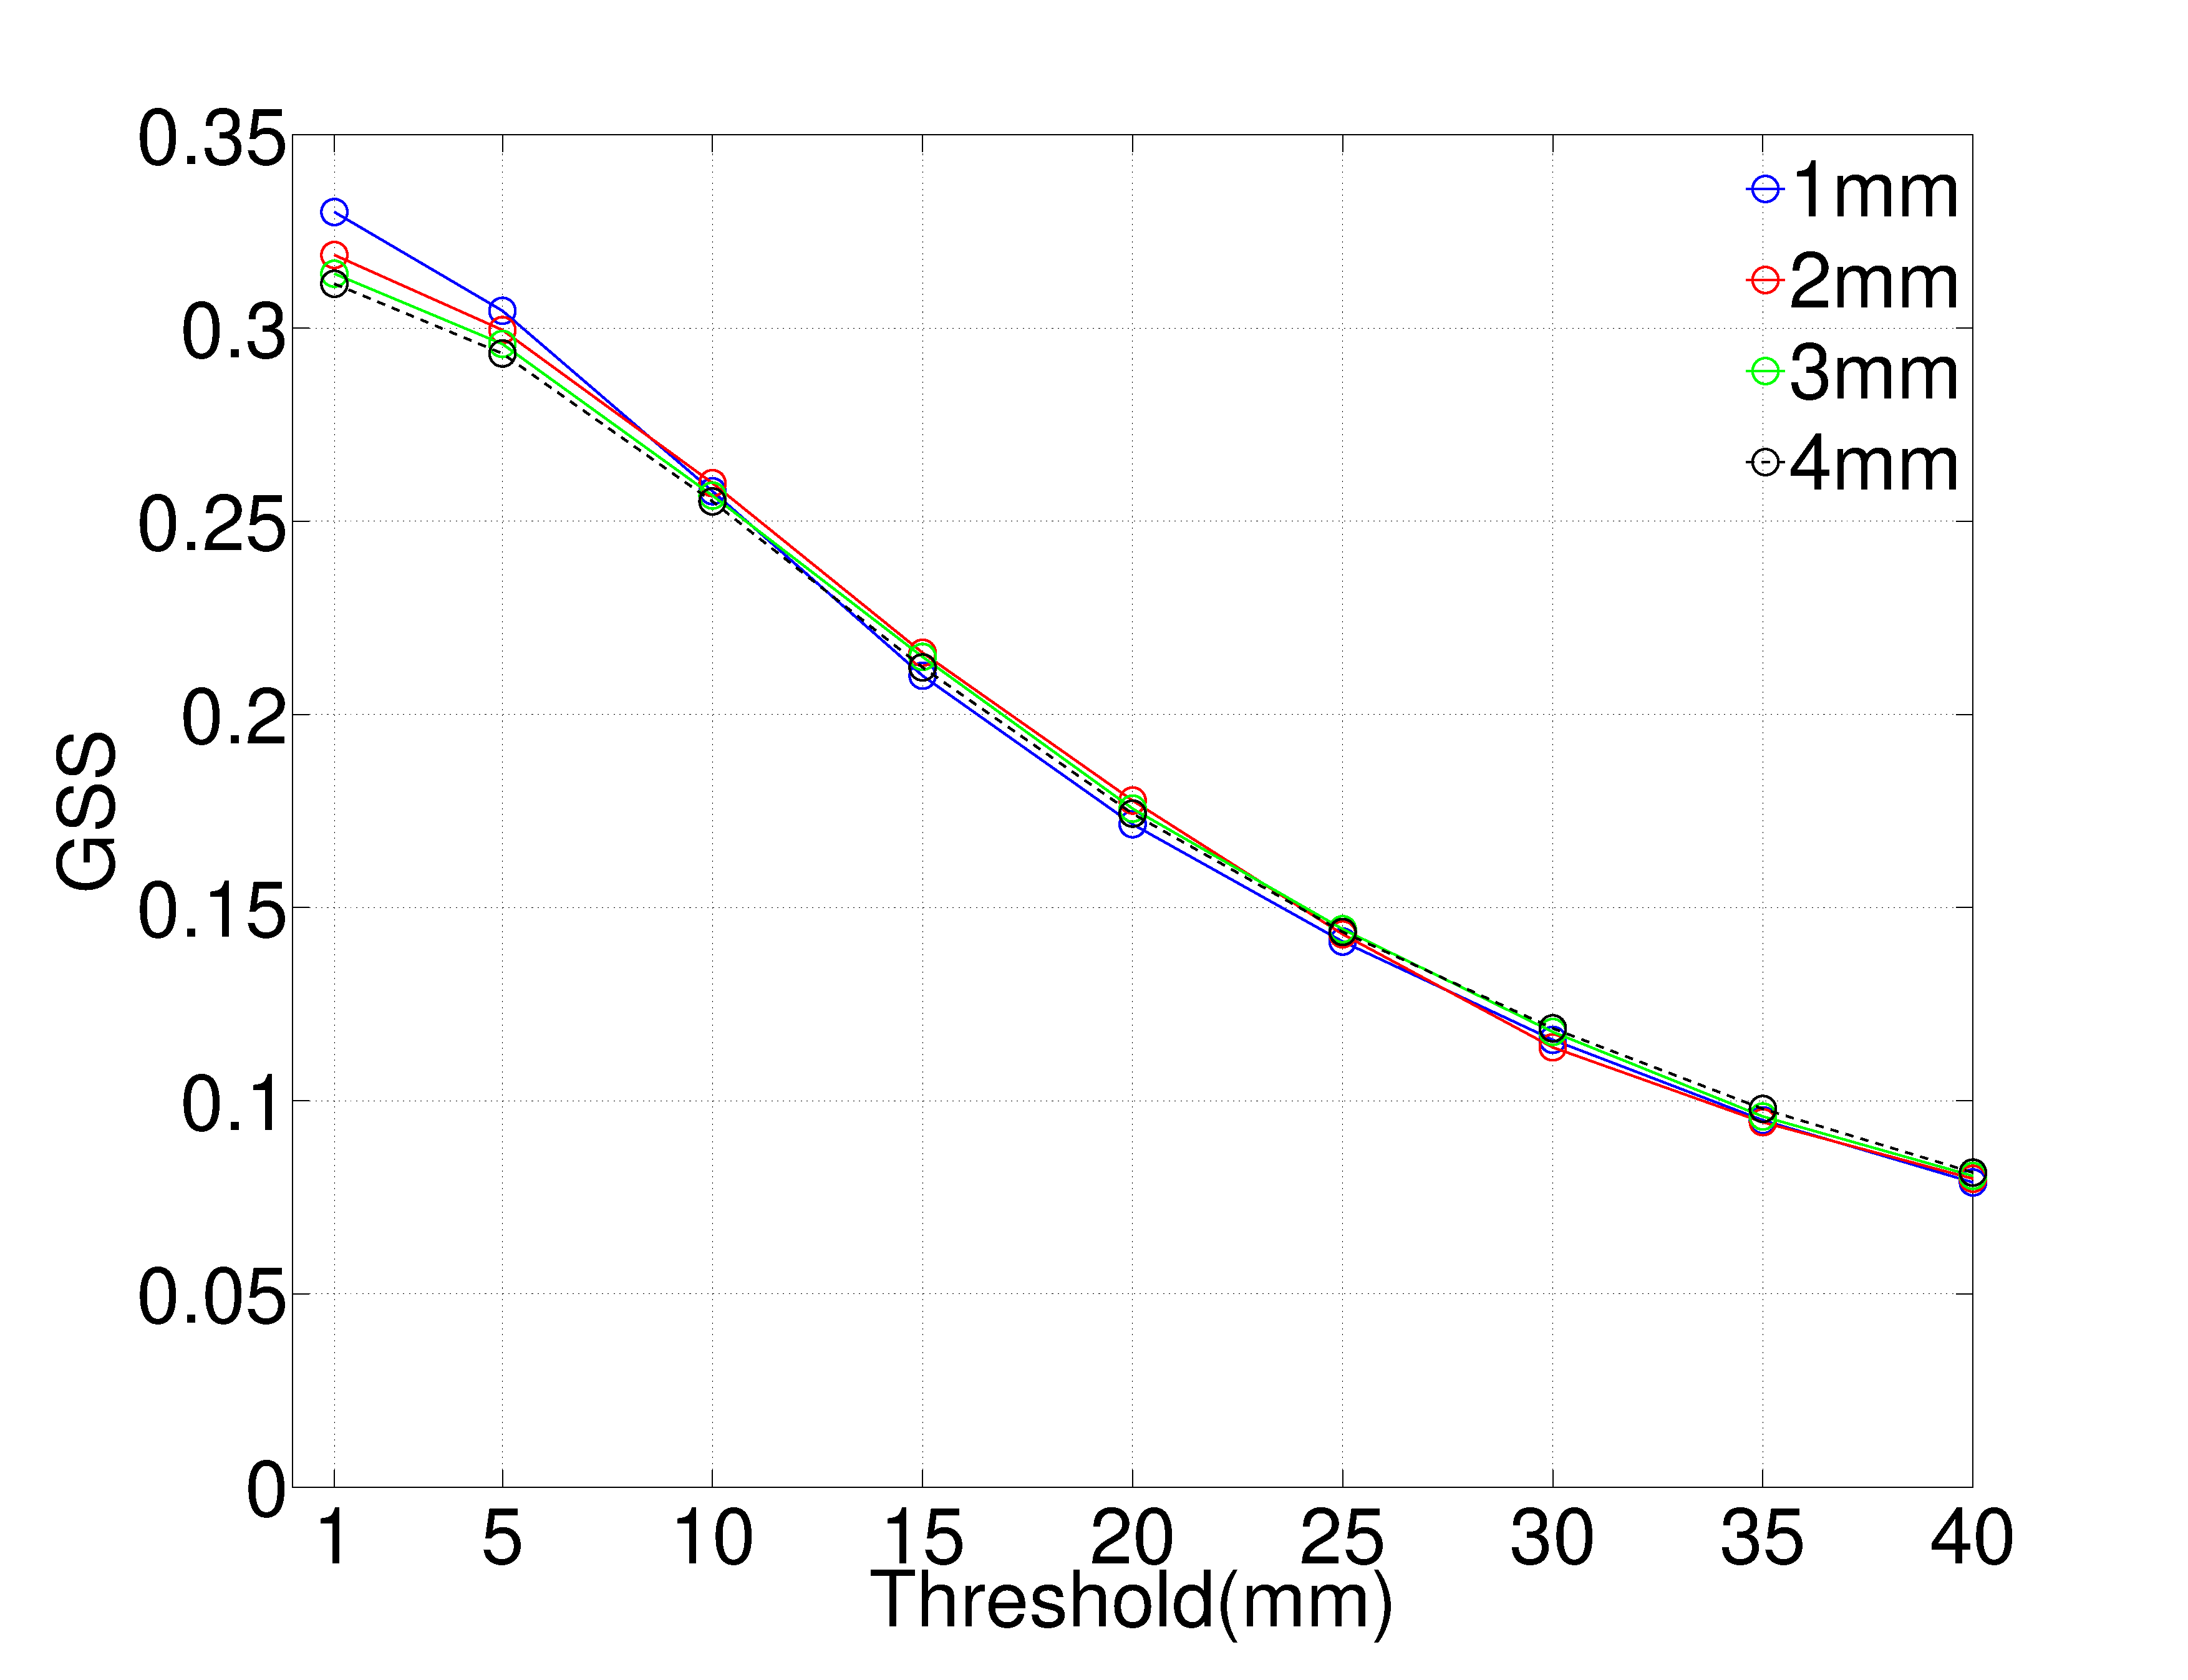
\includegraphics[width=0.5\linewidth]{./figures/gss_24h_error.eps}
\caption{Threshold series of GSS for 24-h accumulated precipitation using the different precipitation errors (1mm, 2mm, 3mm, 4mm).}\label{obserror_test}
\end{figure}

\newpage
\begin{figure}
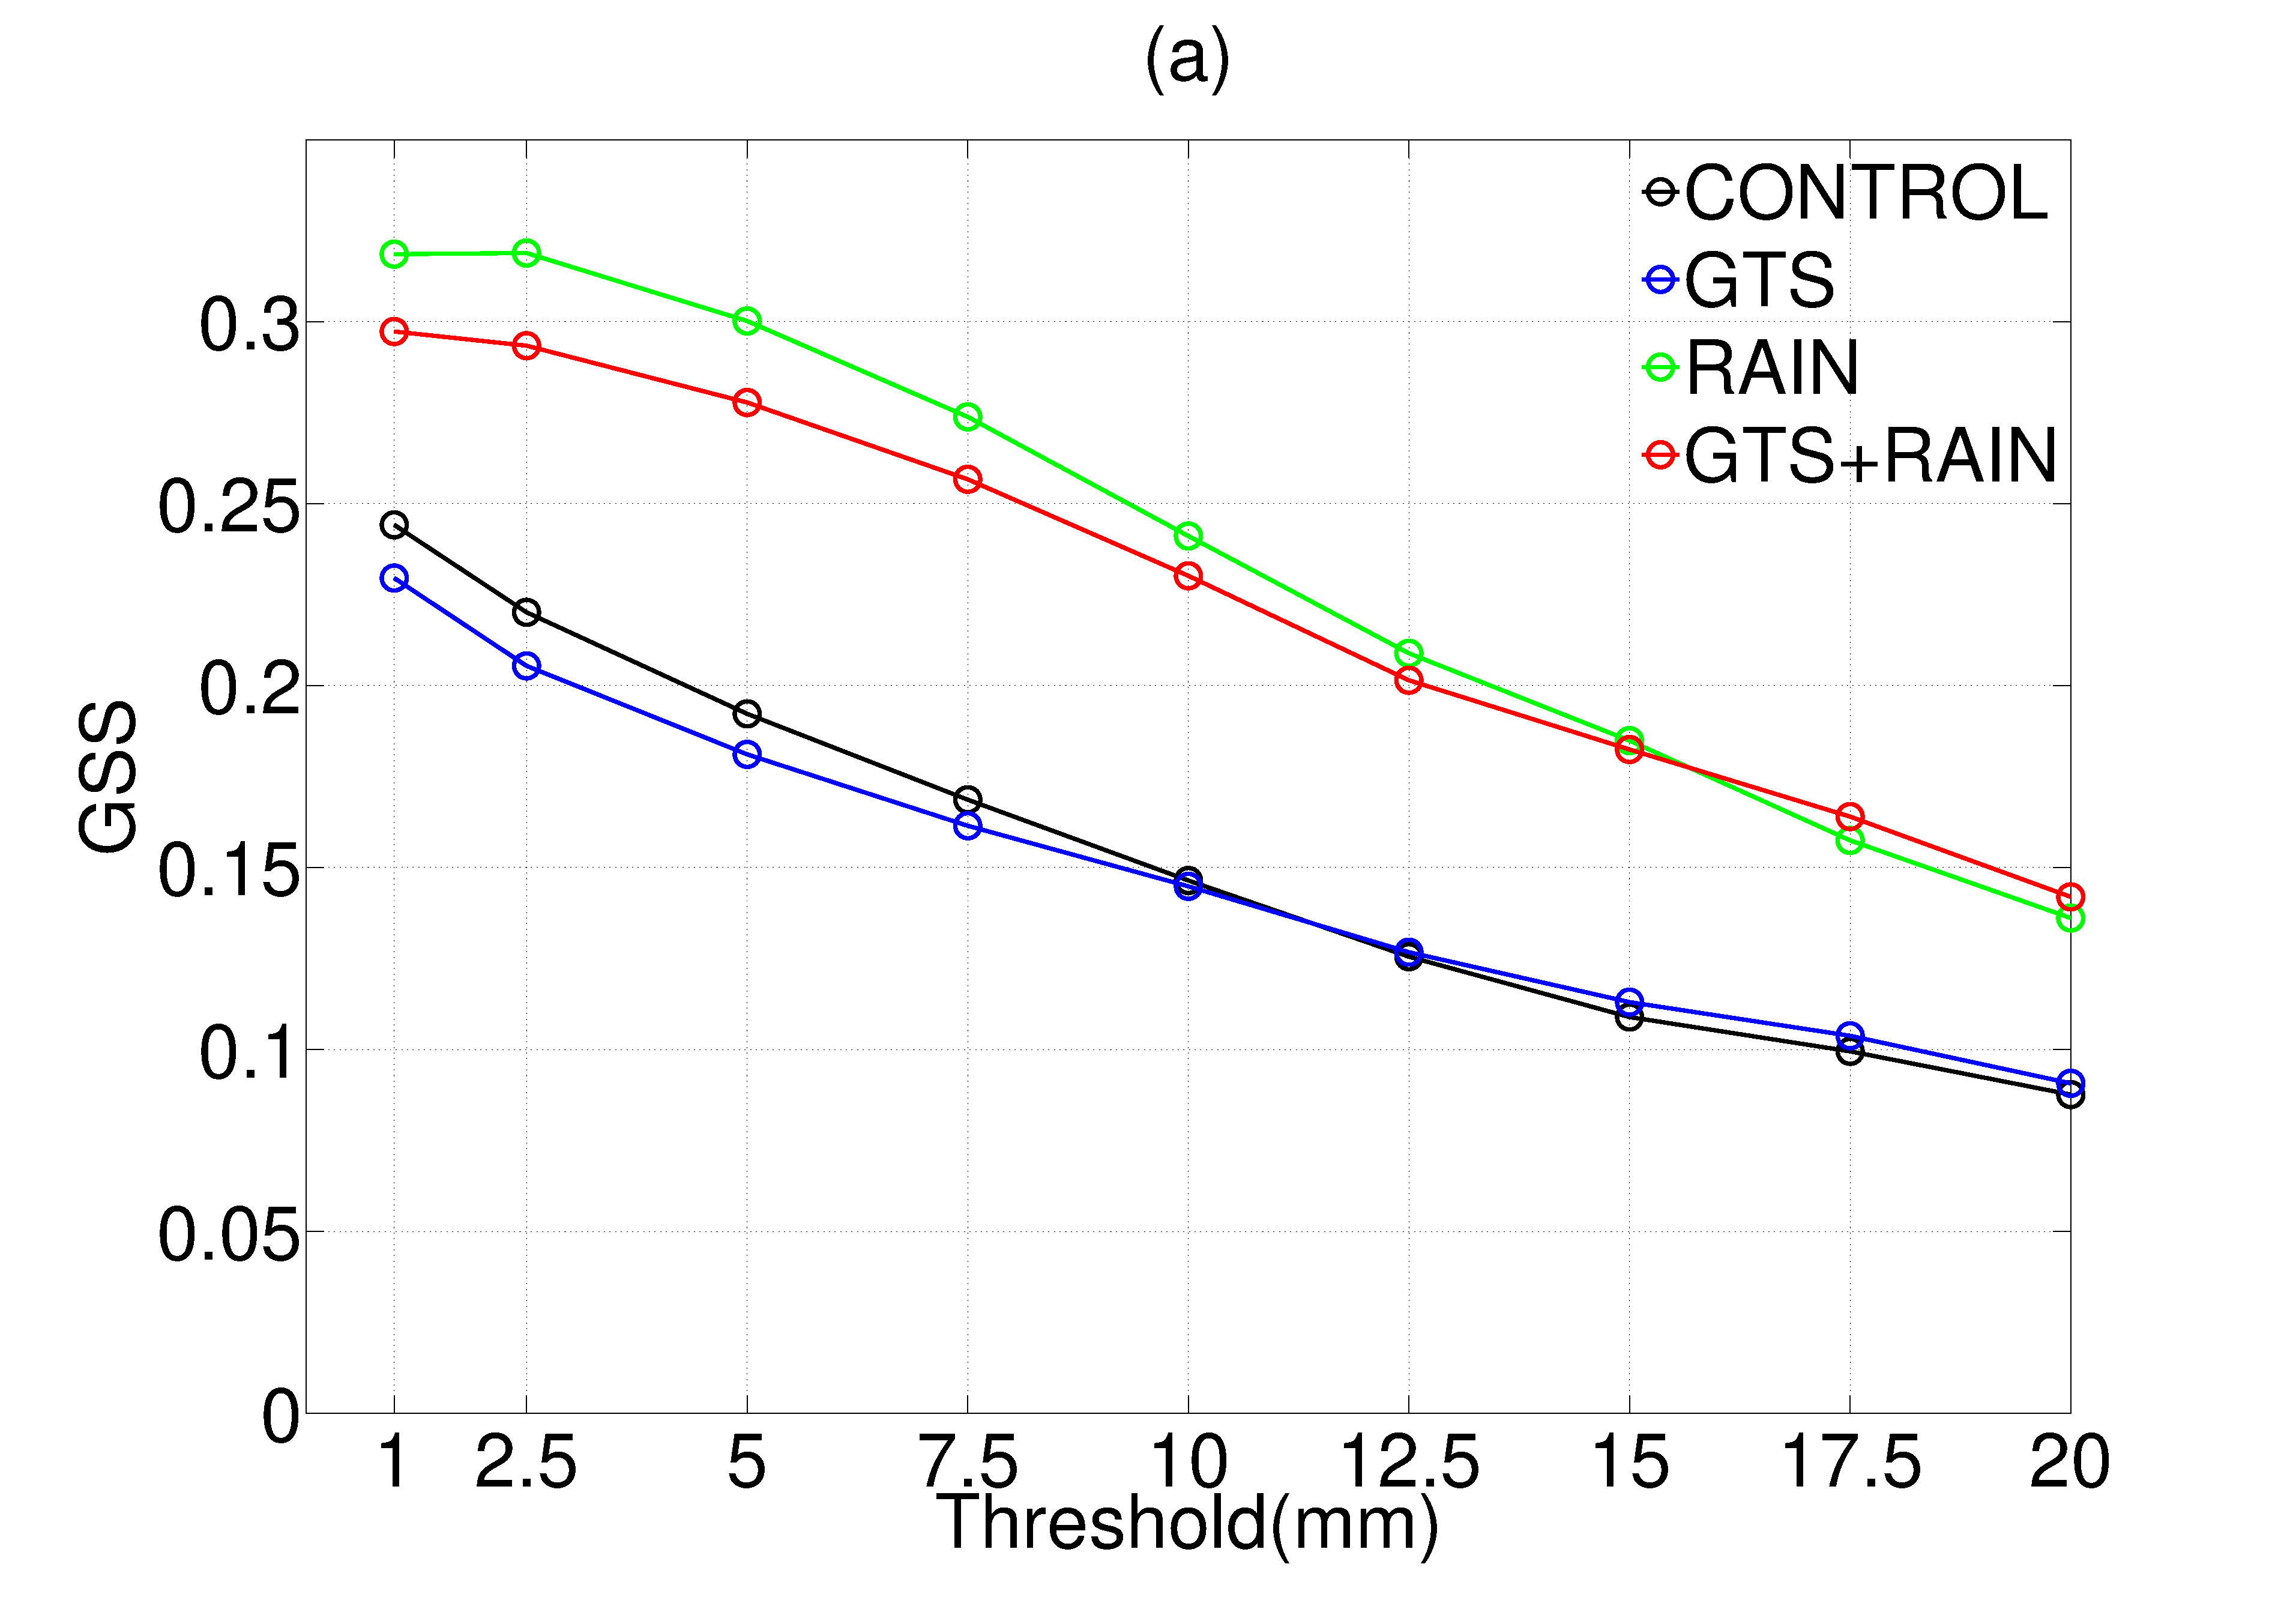
\includegraphics[width=0.5\linewidth]{./figures/GSS_06.eps}
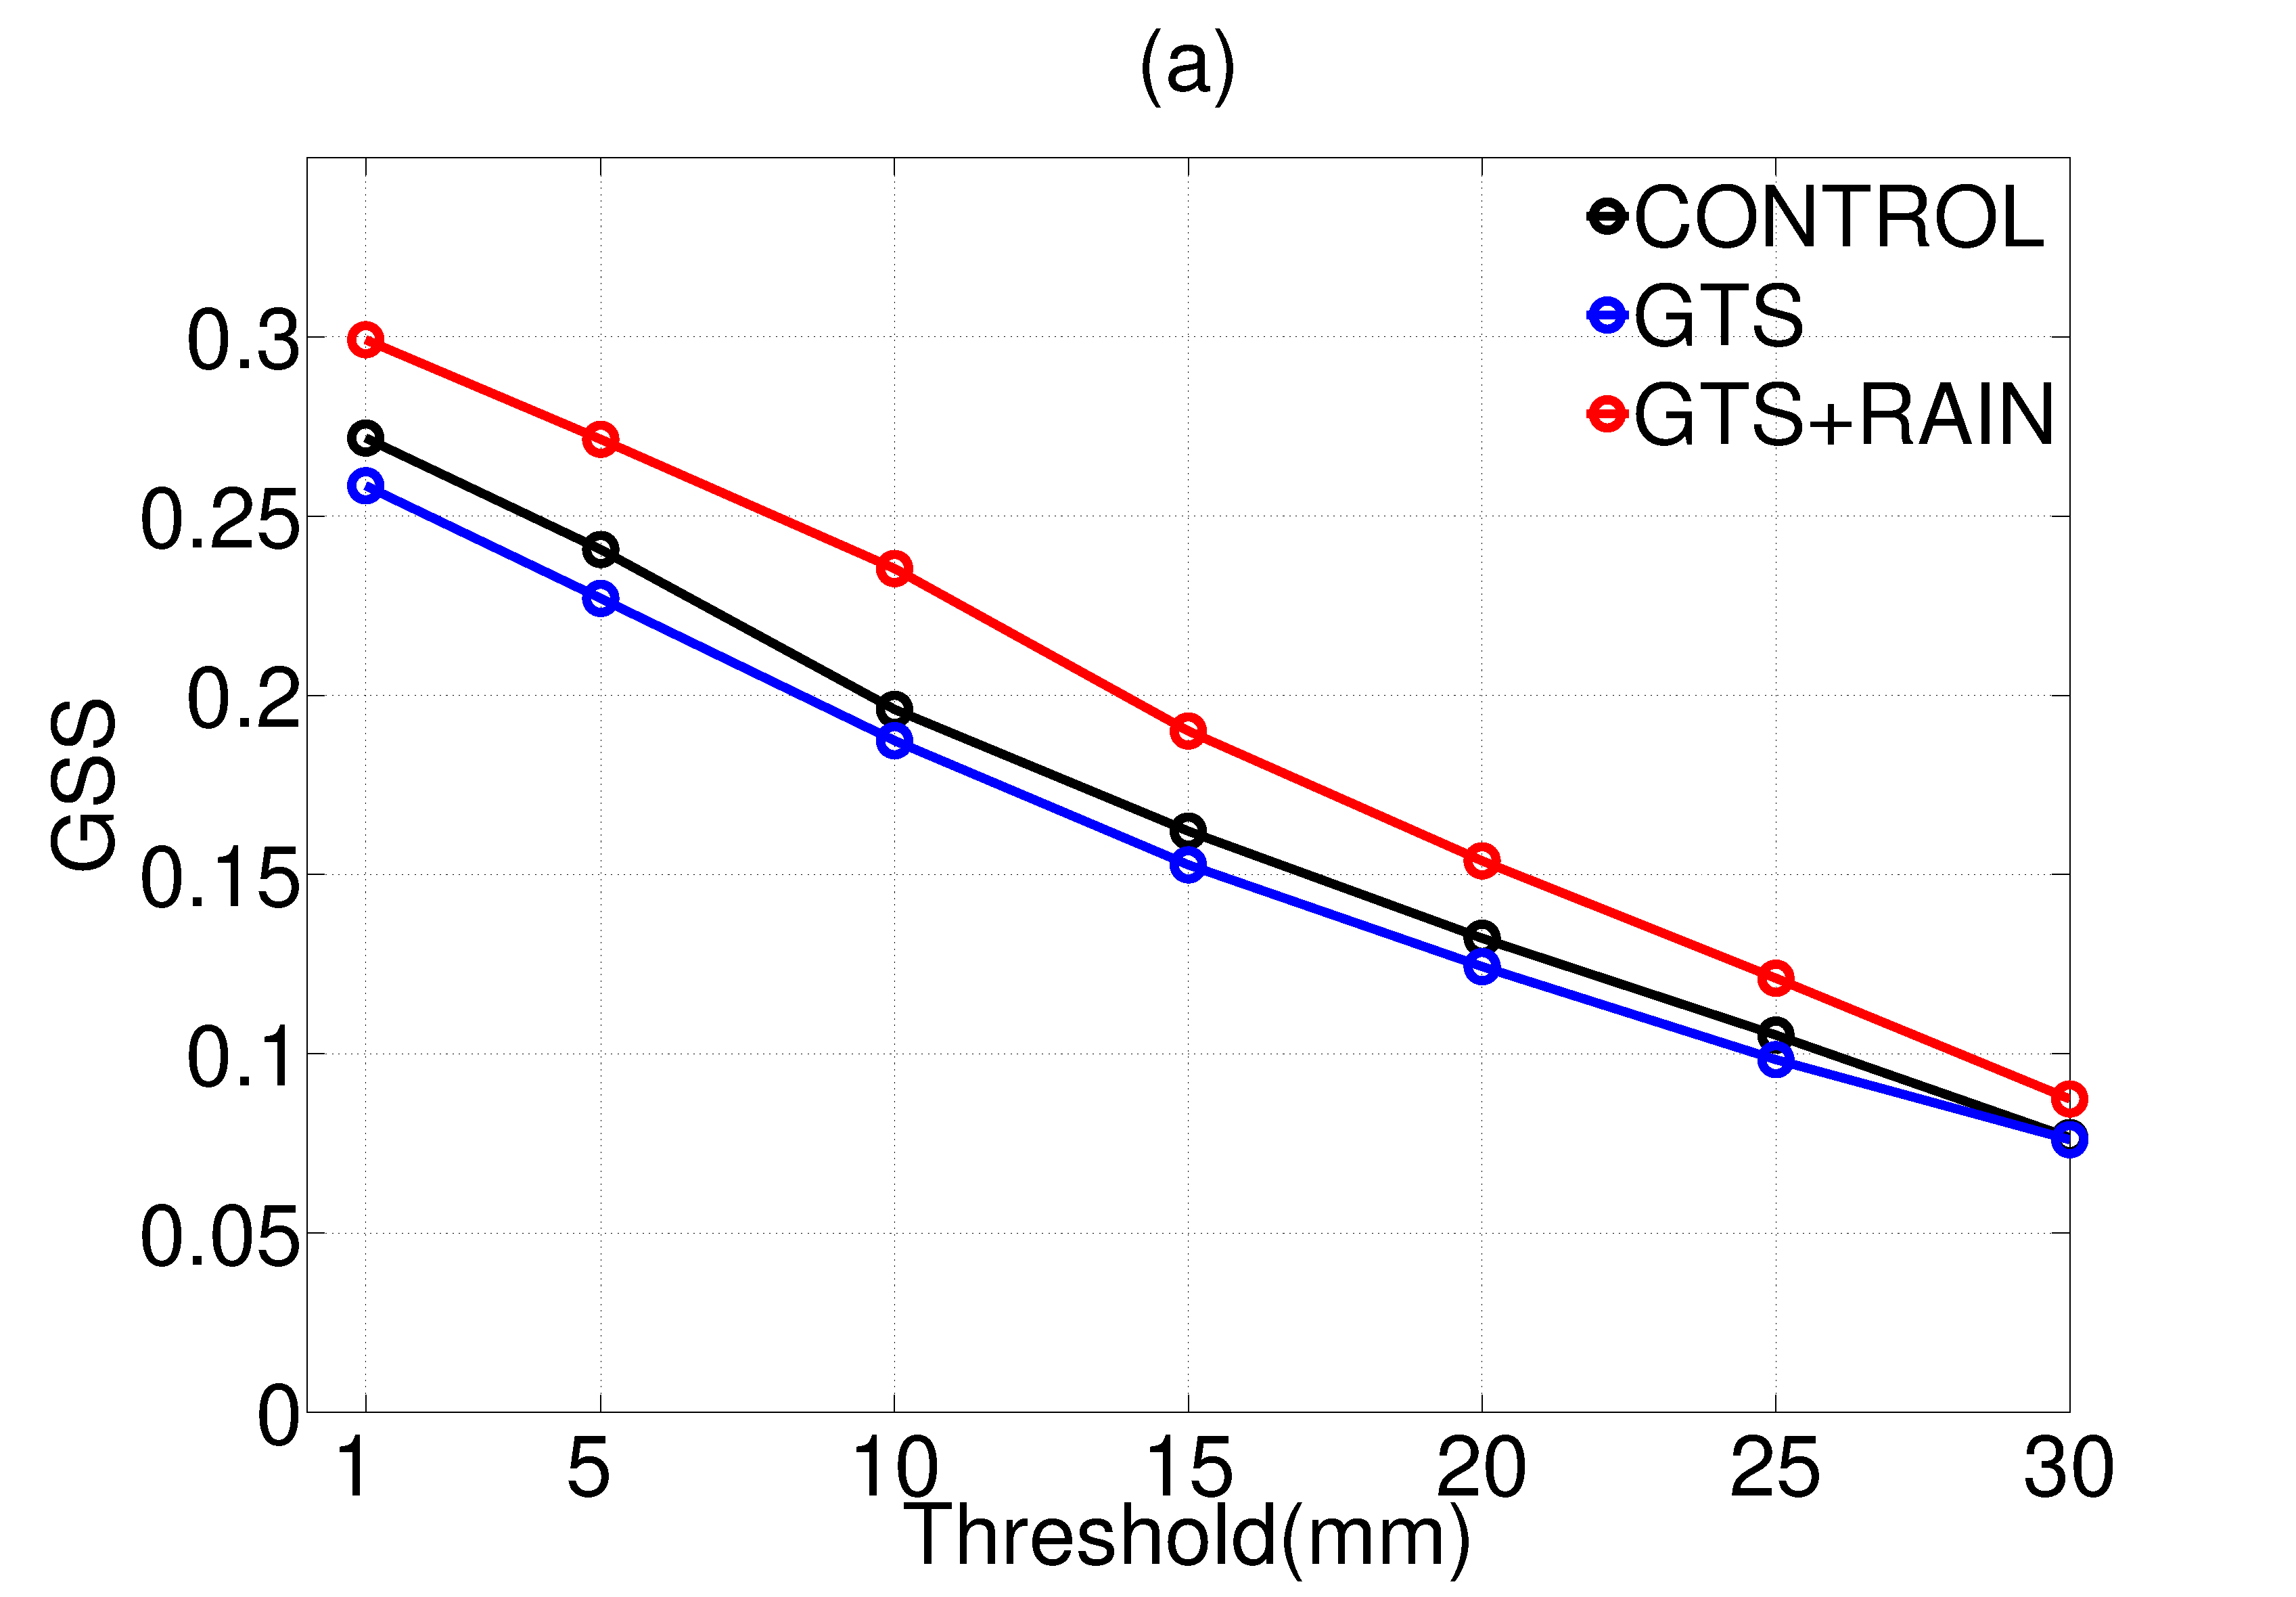
\includegraphics[width=0.5\linewidth]{./figures/GSS_12.eps}
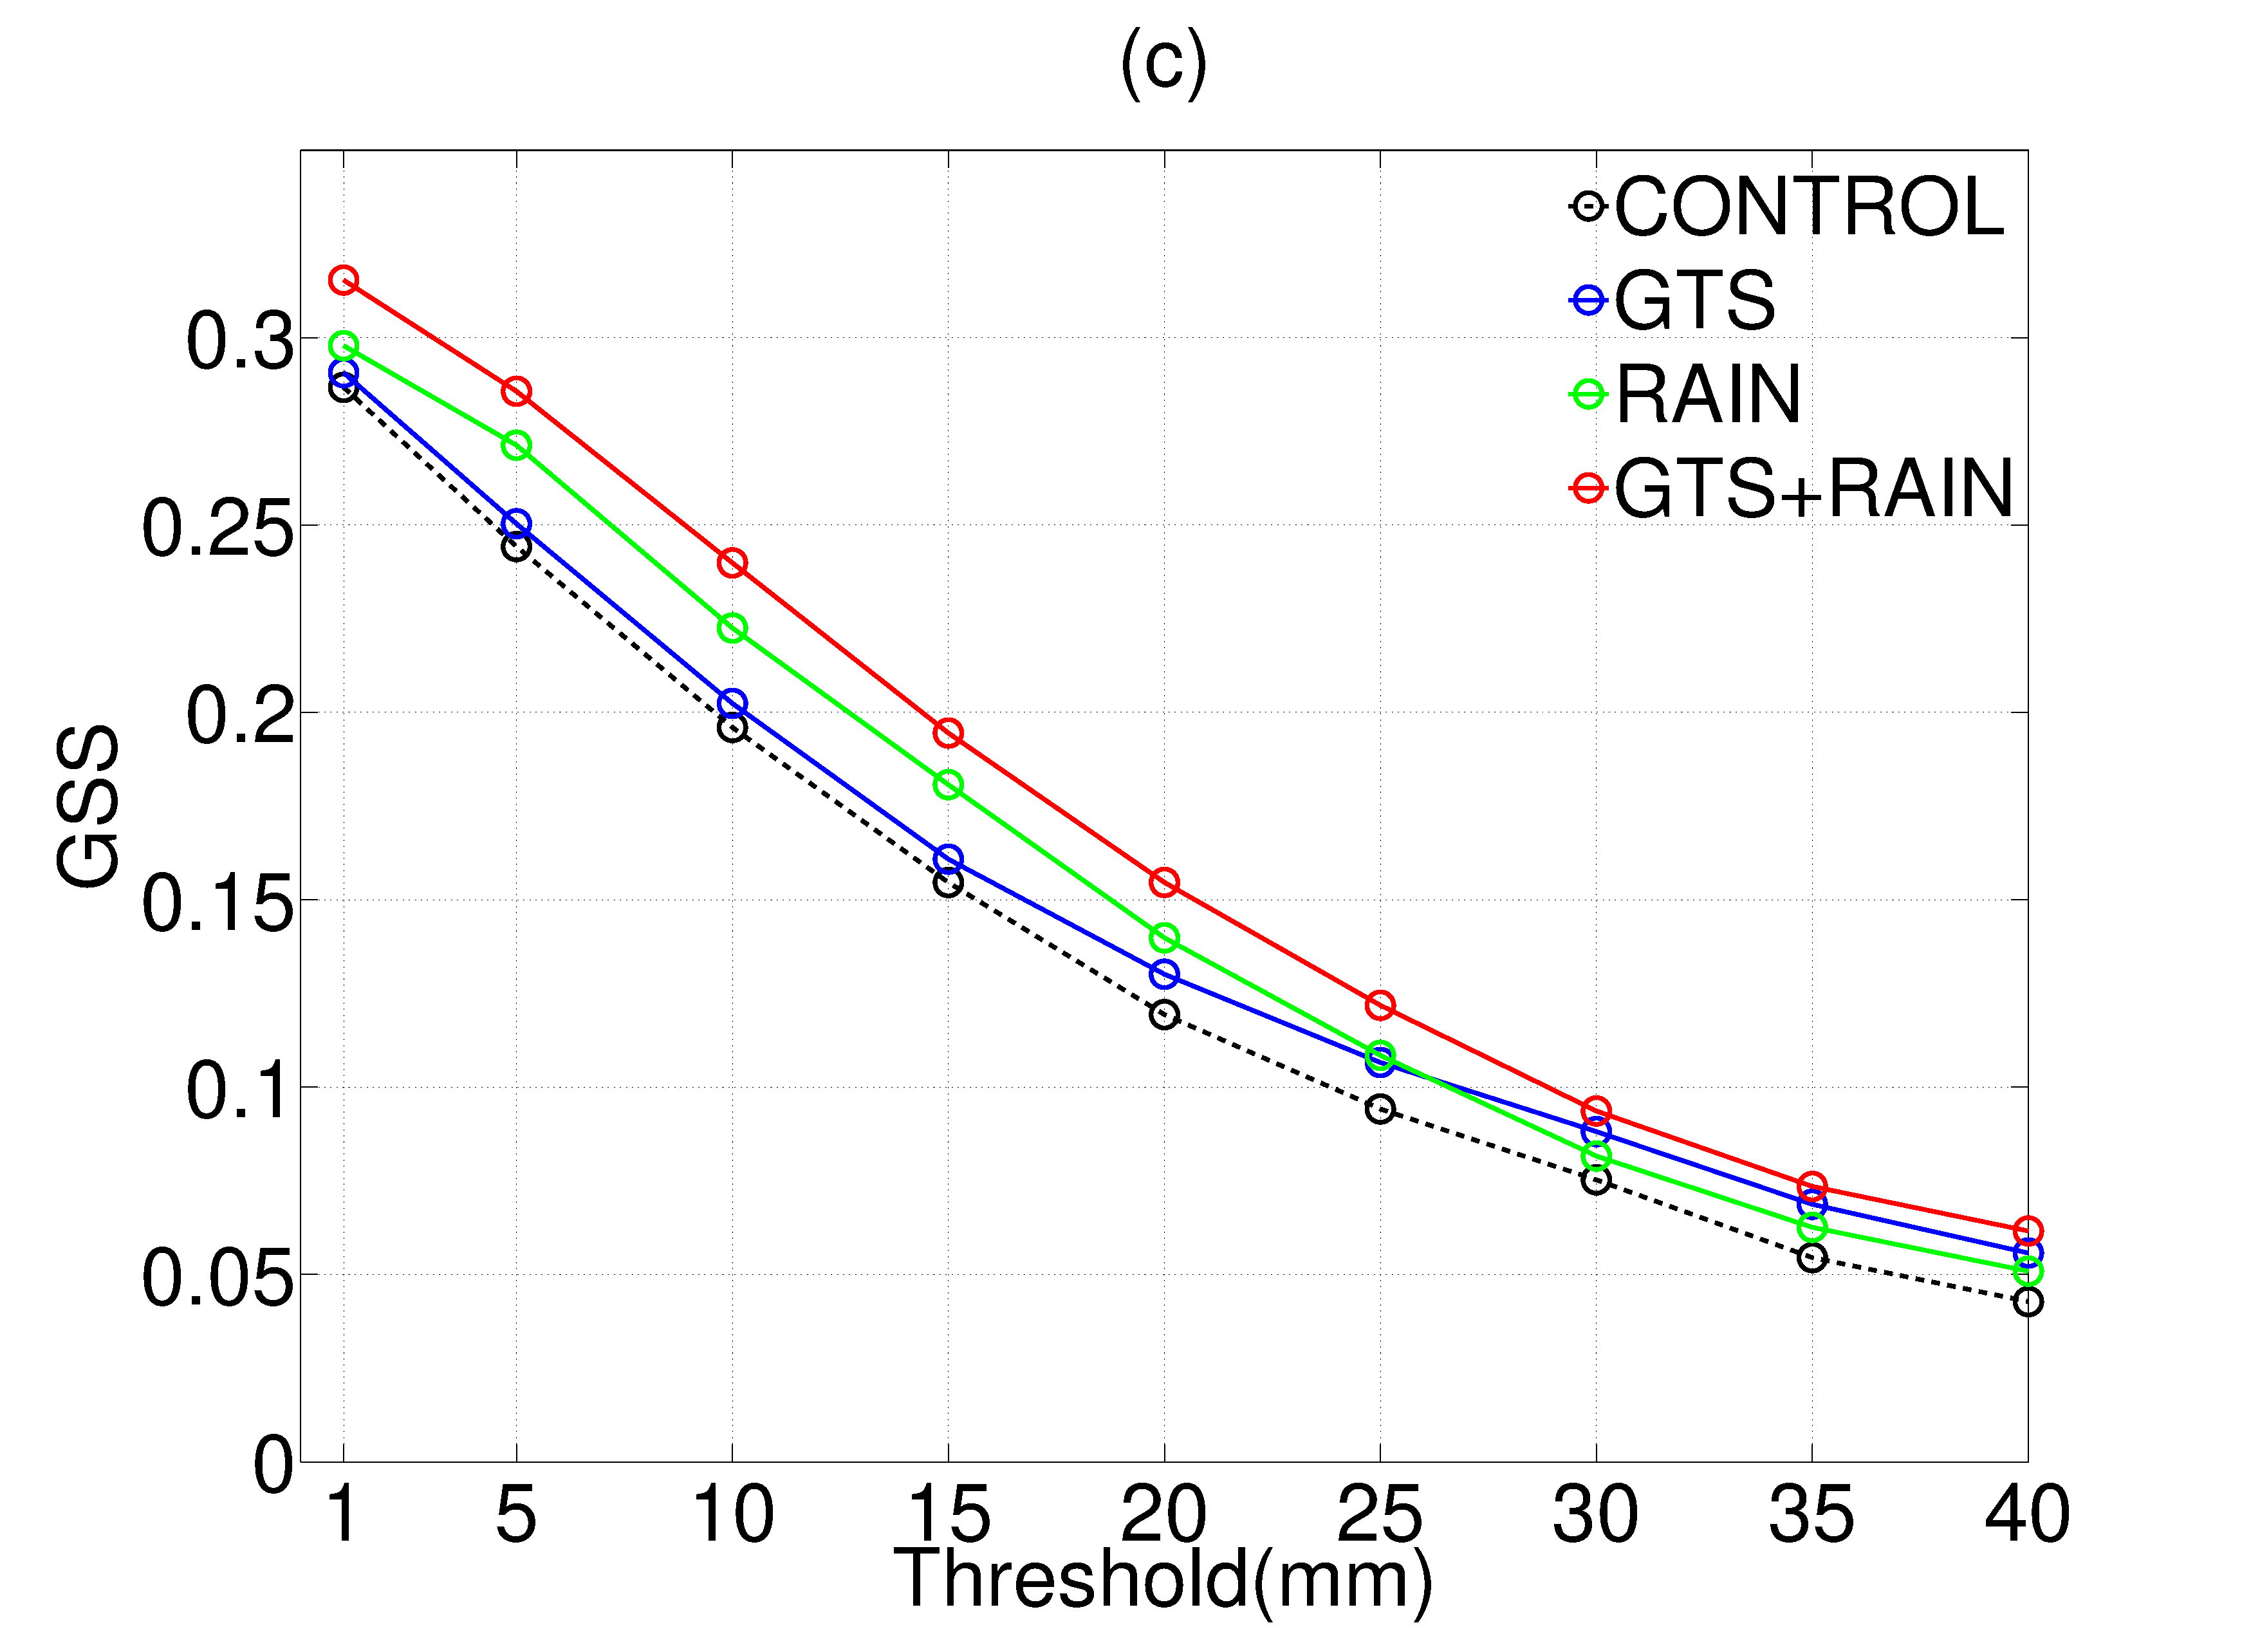
\includegraphics[width=0.5\linewidth]{./figures/GSS_18.eps}
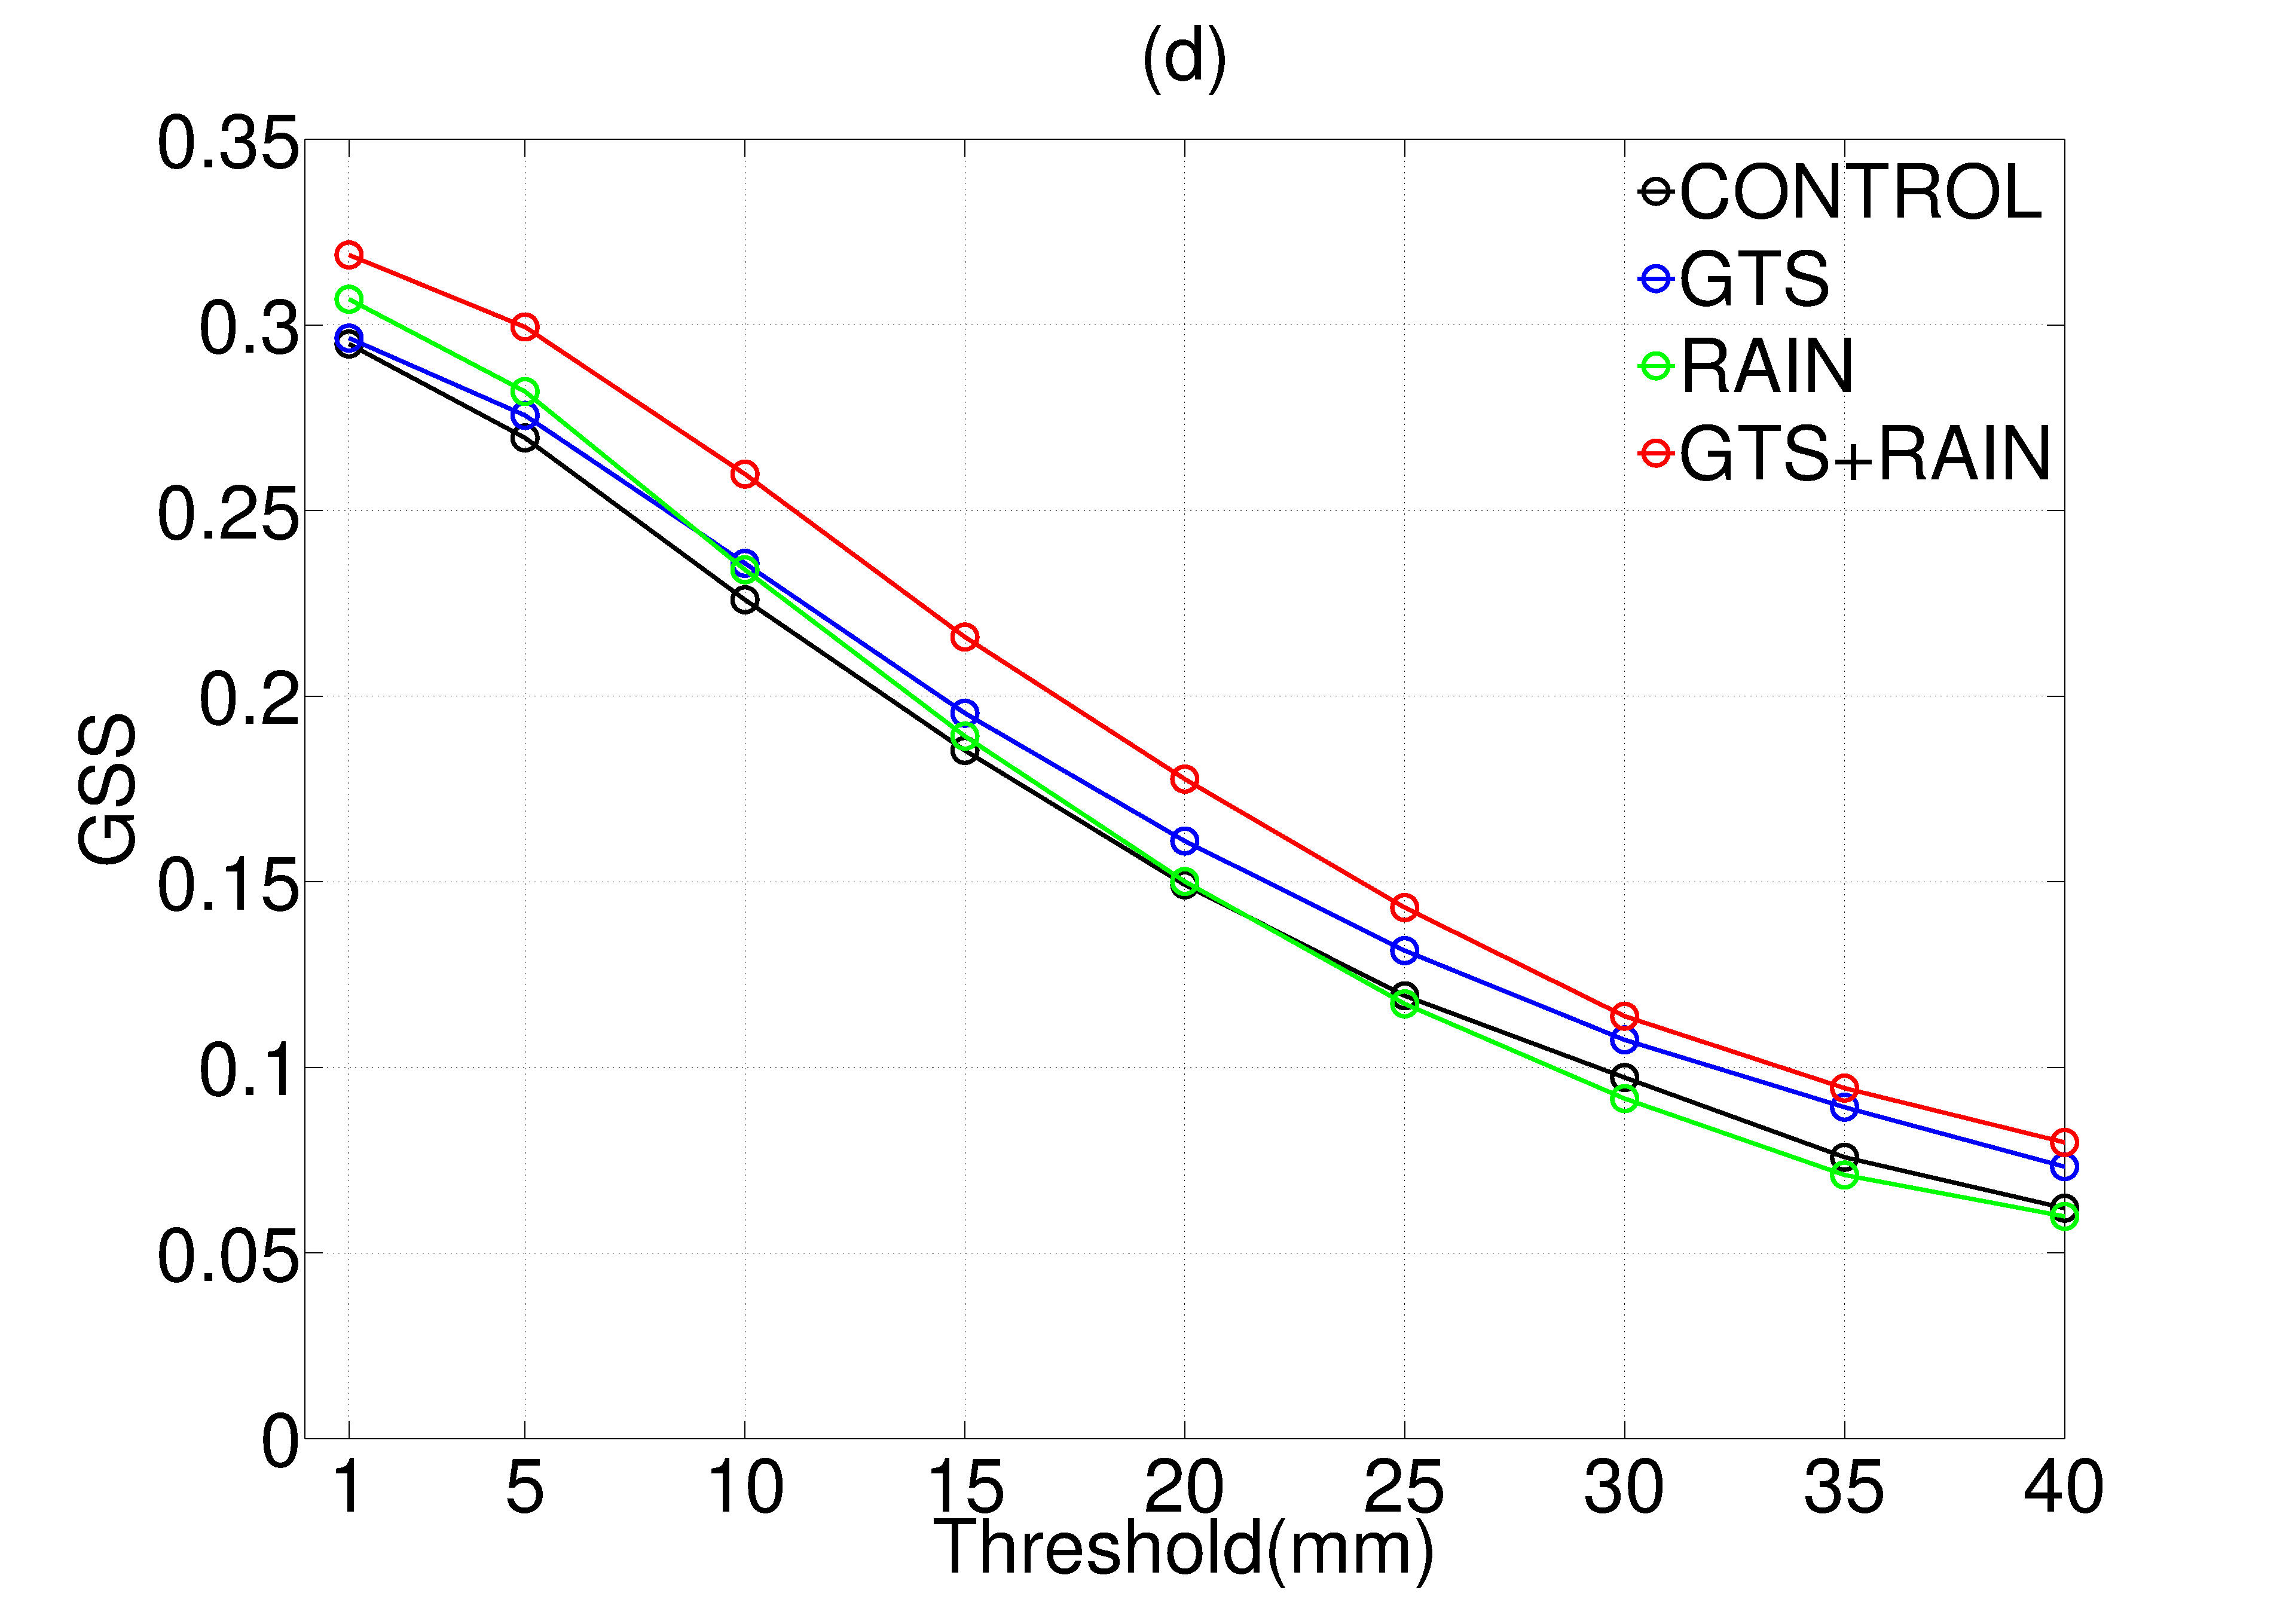
\includegraphics[width=0.5\linewidth]{./figures/GSS_24.eps}
\caption{Threshold series of GSS for 6-h (a), 12-h (b), 18-h (c), and 24-h (d) accumulated precipitation from the experiment CONTROL, GTS, RAIN, GTS+RAIN. }\label{gss_12h}
\end{figure}

%\newpage
%\begin{figure}
%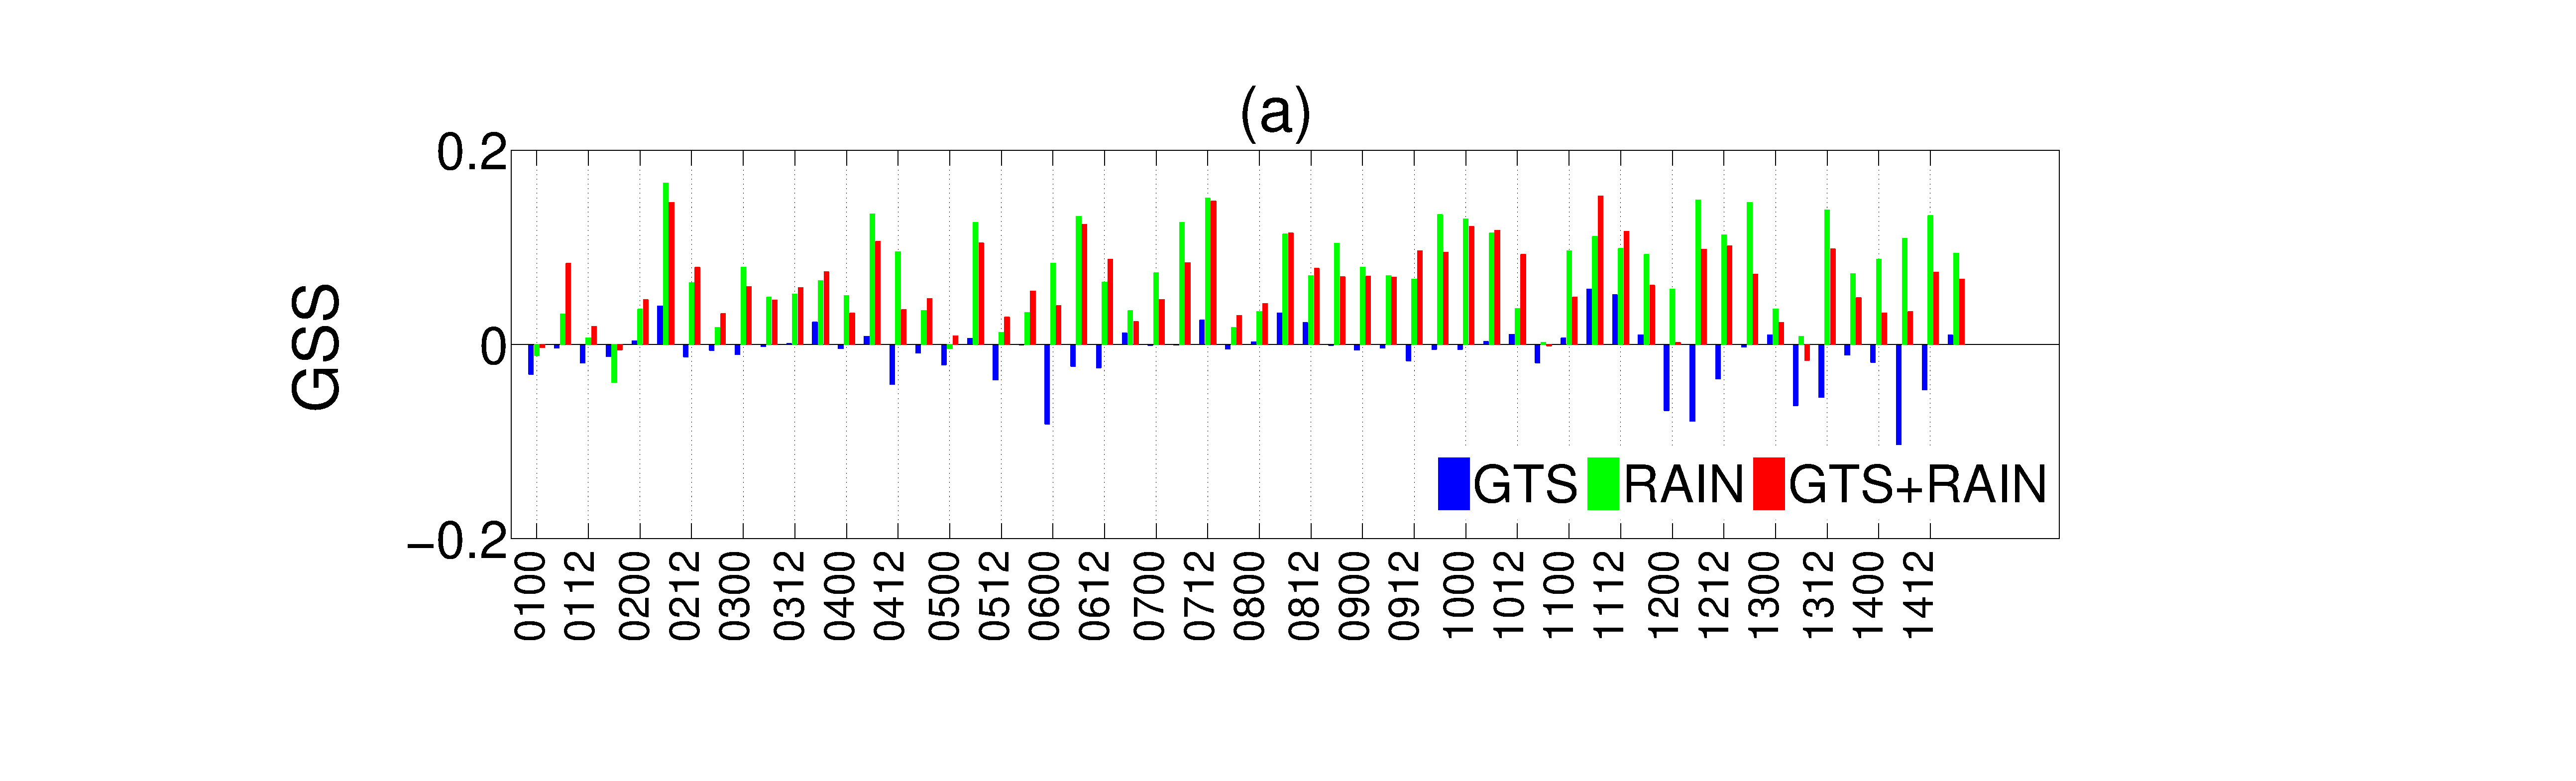
\includegraphics[width=0.8\linewidth]{./figures/GSS_TIMESERI_06H.eps}
%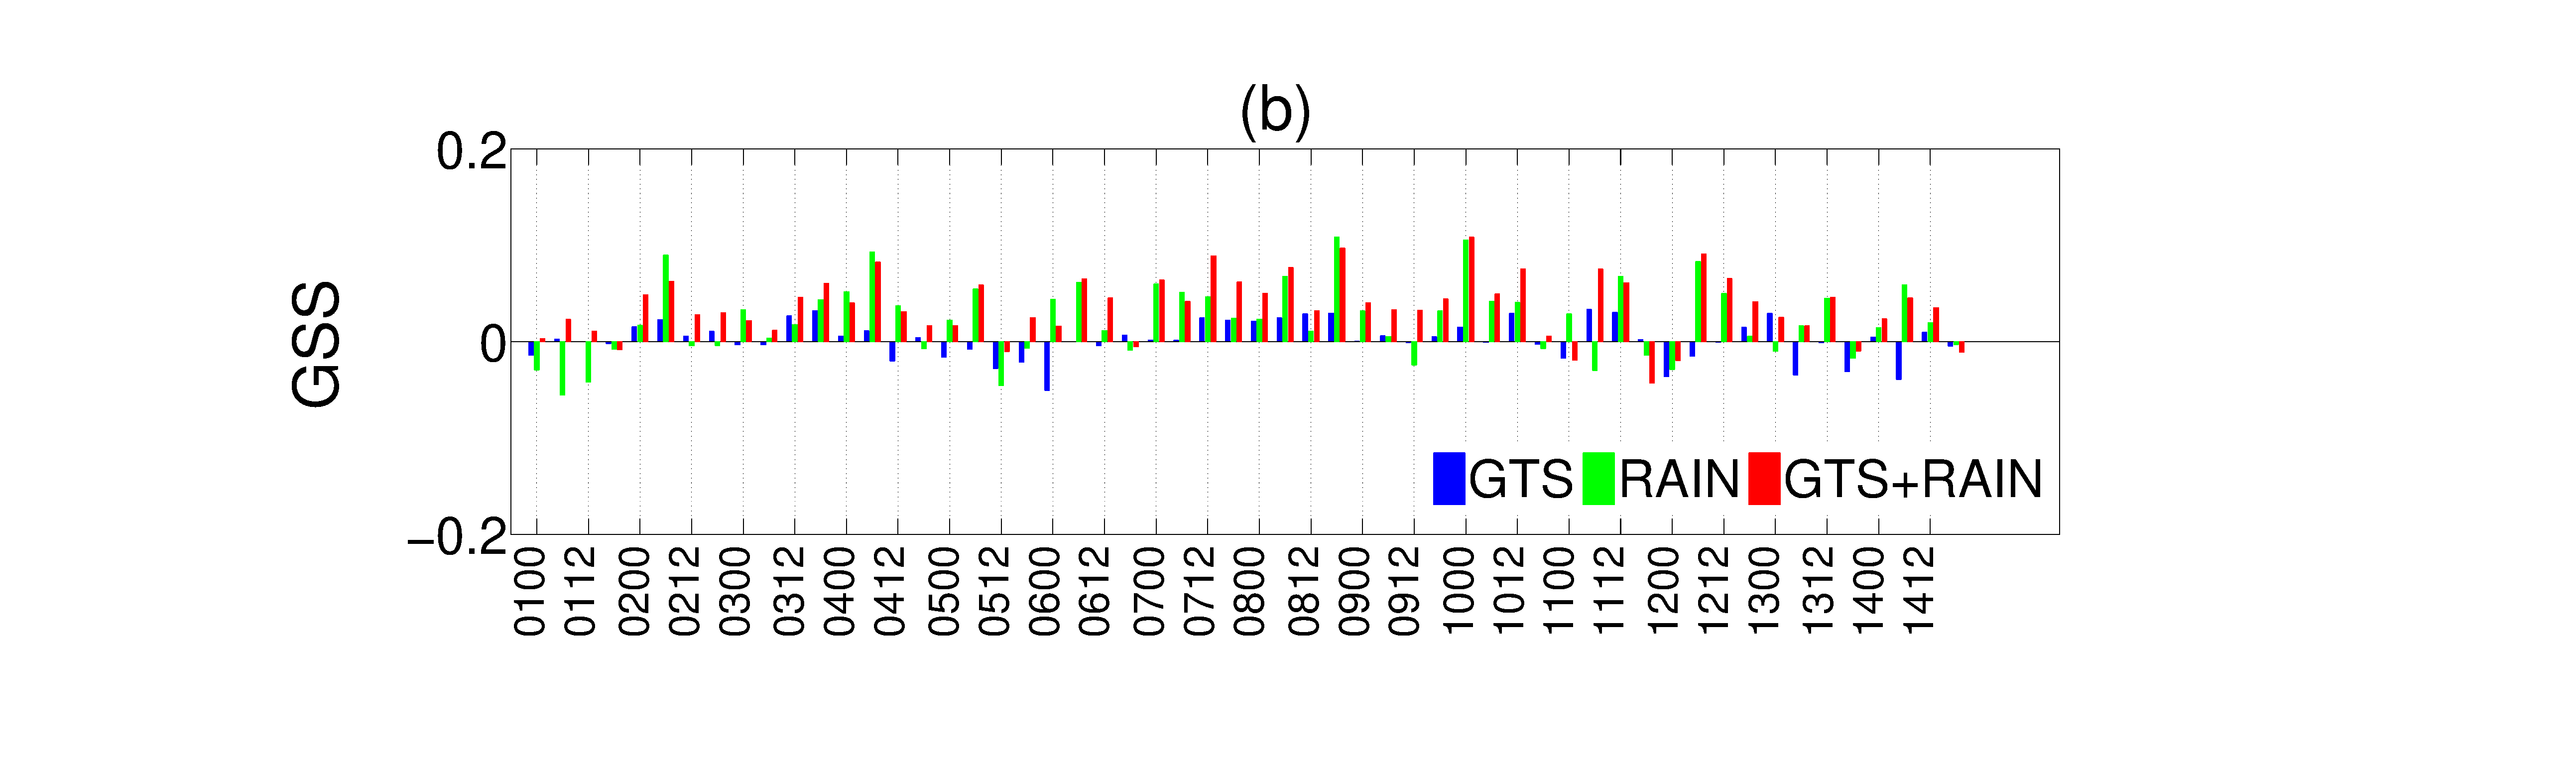
\includegraphics[width=0.8\linewidth]{./figures/GSS_TIMESERI_12H.eps}
%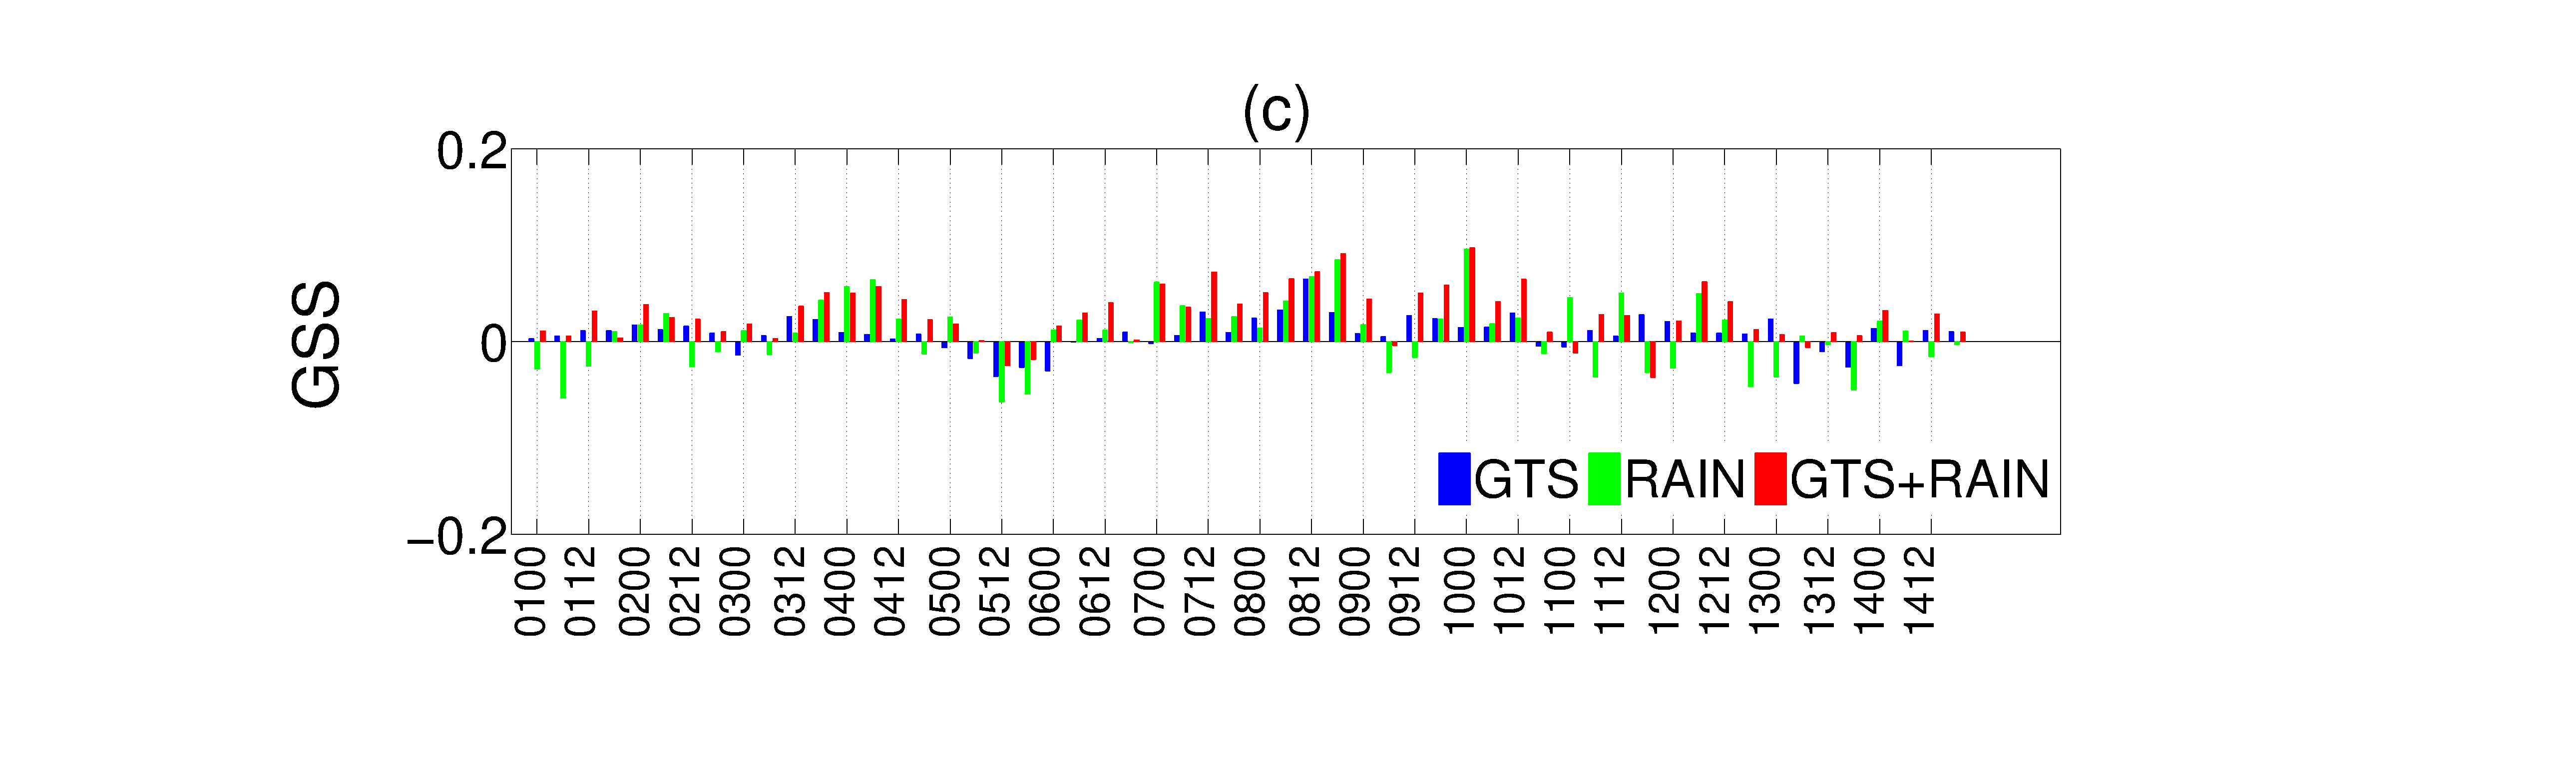
\includegraphics[width=0.8\linewidth]{./figures/GSS_TIMESERI_18H.eps}
%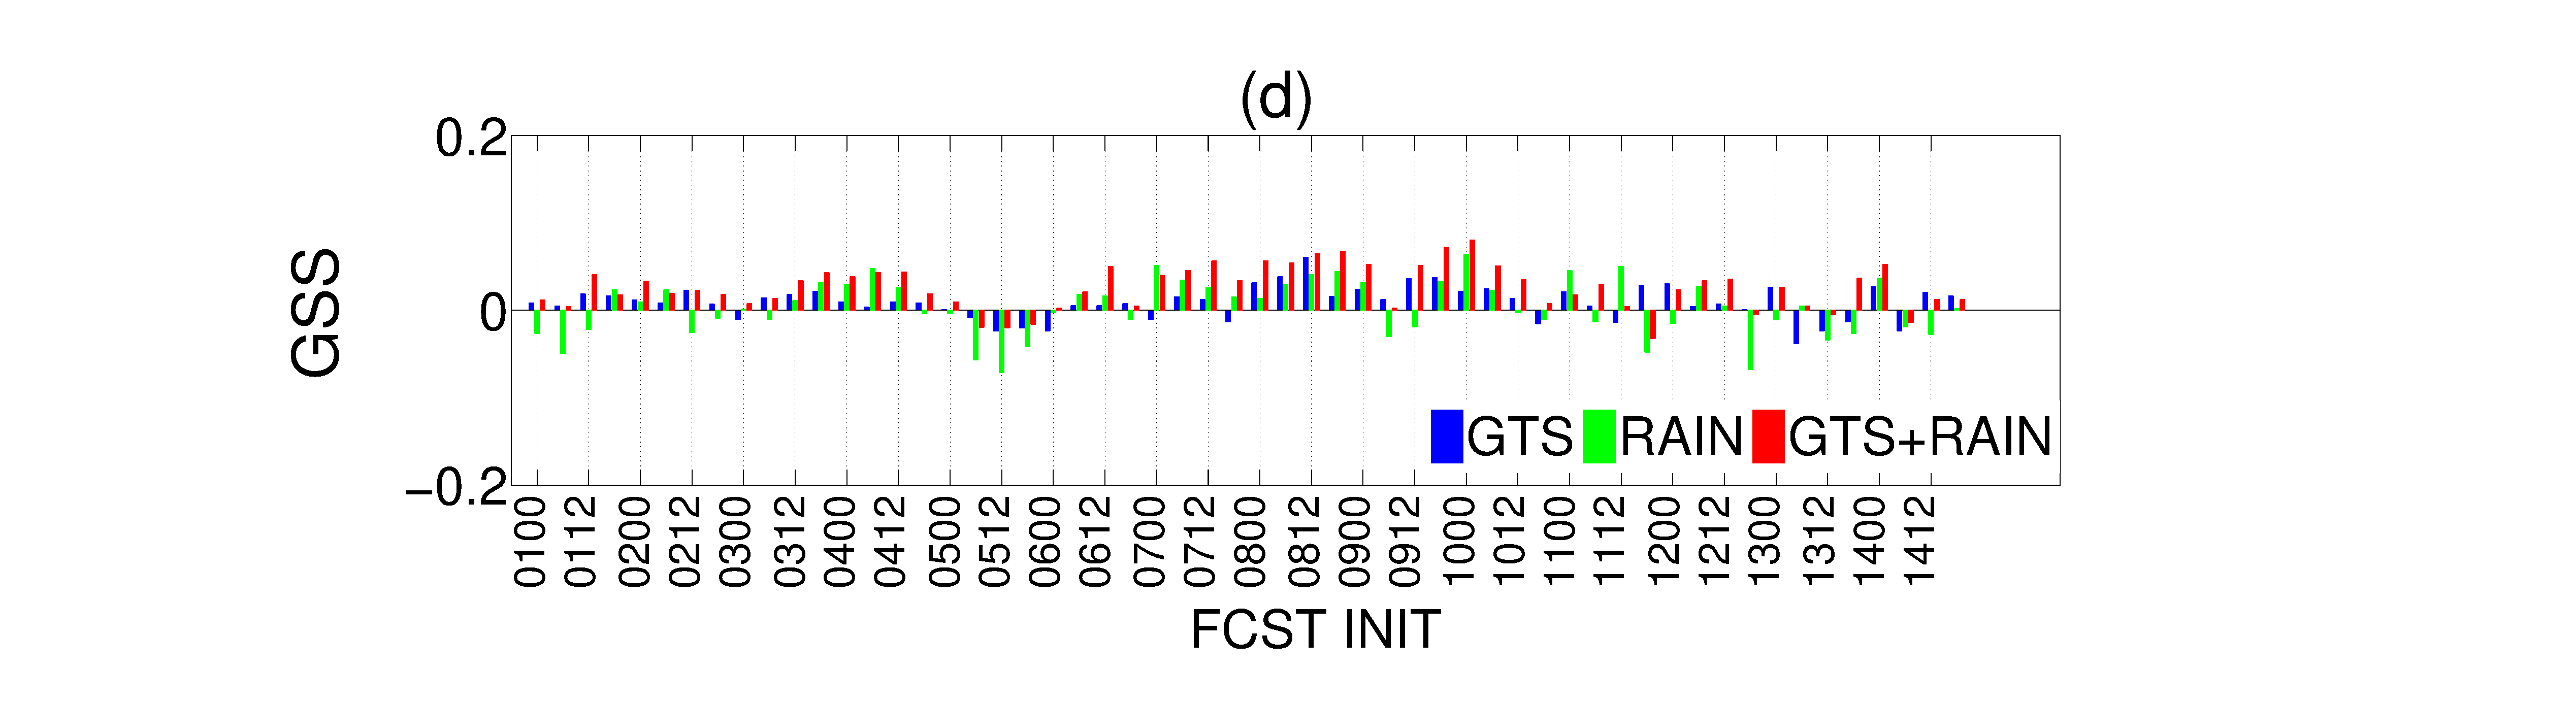
\includegraphics[width=0.8\linewidth]{./figures/GSS_TIMESERI_24H.eps}
%\caption{Time series of Gilberty Skill Score (GSS) from 0000 UTC 1 to 1800 UTC 14 June 2010. The 6-h (a), 12-h (b), 18-h (c) and 24-h (d) accumulated precipitation from the experiment CONTROL, GTS, RAIN, GTS+RAIN are verified against NCEP Stage IV gridded precipitation. The results have been averaged across all the thresholds.}\label{timeser}
%\end{figure}

%\newpage
%\begin{figure}
%\includegraphics[width=0.4\linewidth]{./figures/st4_copy.pdf}

%\includegraphics[width=0.4\linewidth]{./figures/control_copy.pdf}

%\includegraphics[width=0.4\linewidth]{./figures/gts_copy.pdf}

%\includegraphics[width=0.4\linewidth]{./figures/gts+rain_copy.pdf}
%\includegraphics[width=0.4\linewidth]{gts+rain.eps}
%\caption{12-h accumulated precipitation (mm) from 0000 UTC to 1200 UTC 10 June 2010. (a) NCEP Stage-IV (b) CONTROL (c) GTS (d) GTS+RAIN. }\label{rainfall}
%\end{figure}

%\begin{table}
%\caption{Table caption}\label{sampletable}
%\begin{tabular}{l l l}
%\hline
%\textbf{Treatments} & \textbf{Response 1} & \textbf{Response 2}\\
%\hline
%Treatment 1 & 0.0003262 & 0.562 \\
%Treatment 2 & 0.0015681 & 0.910 \\
%Treatment 3 & 0.0009271 & 0.296 \\
%\hline
%\end{tabular}
%\end{table}

\end{document}

%%%%%%%%%%%%%%%%%%%%%%%%%%%%%%%%%%%%%%%%%%%%%%%%%%%%%%%%%%%%%%%

More Information and Advice:

%% ------------------------------------------------------------------------ %%
%
%  SECTION HEADS
%
%% ------------------------------------------------------------------------ %%

% Capitalize the first letter of each word (except for
% prepositions, conjunctions, and articles that are
% three or fewer letters).

% AGU follows standard outline style; therefore, there cannot be a section 1 without
% a section 2, or a section 2.3.1 without a section 2.3.2.
% Please make sure your section numbers are balanced.
% ---------------
% Level 1 head
%
% Use the \section{} command to identify level 1 heads;
% type the appropriate head wording between the curly
% brackets, as shown below.
%
%An example:
%\section{Level 1 Head: Introduction}
%
% ---------------
% Level 2 head
%
% Use the \subsection{} command to identify level 2 heads.
%An example:
%\subsection{Level 2 Head}
%
% ---------------
% Level 3 head
%
% Use the \subsubsection{} command to identify level 3 heads
%An example:
%\subsubsection{Level 3 Head}
%
%---------------
% Level 4 head
%
% Use the \subsubsubsection{} command to identify level 3 heads
% An example:
%\subsubsubsection{Level 4 Head} An example.
%
%% ------------------------------------------------------------------------ %%
%
%  IN-TEXT LISTS
%
%% ------------------------------------------------------------------------ %%
%
% Do not use bulleted lists; enumerated lists are okay.
% \begin{enumerate}
% \item
% \item
% \item
% \end{enumerate}
%
%% ------------------------------------------------------------------------ %%
%
%  EQUATIONS
%
%% ------------------------------------------------------------------------ %%

% Single-line equations are centered.
% Equation arrays will appear left-aligned.

Math coded inside display math mode \[ ...\]
 will not be numbered, e.g.,:
 \[ x^2=y^2 + z^2\]

 Math coded inside \begin{equation} and \end{equation} will
 be automatically numbered, e.g.,:
 \begin{equation}
 x^2=y^2 + z^2
 \end{equation}

% IF YOU HAVE MULTI-LINE EQUATIONS, PLEASE
% BREAK THE EQUATIONS INTO TWO OR MORE LINES
% OF SINGLE COLUMN WIDTH (20 pc, 8.3 cm)
% using double backslashes (\\).

% To create multiline equations, use the
% \begin{eqnarray} and \end{eqnarray} environment
% as demonstrated below.
\begin{eqnarray}
  x_{1} & = & (x - x_{0}) \cos \Theta \nonumber \\
        && + (y - y_{0}) \sin \Theta  \nonumber \\
  y_{1} & = & -(x - x_{0}) \sin \Theta \nonumber \\
        && + (y - y_{0}) \cos \Theta.
\end{eqnarray}

%If you don't want an equation number, use the star form:
%\begin{eqnarray*}...\end{eqnarray*}

% Break each line at a sign of operation
% (+, -, etc.) if possible, with the sign of operation
% on the new line.

% Indent second and subsequent lines to align with the first character following the equal sign on the first line.

% Use an \hspace{} command to insert horizontal space into your equation if necessary. Place an appropriate unit of measure between the curly braces, e.g. \hspace{1in}; you may have to experiment to achieve the correct amount of space.


%% ------------------------------------------------------------------------ %%
%
%  EQUATION NUMBERING: COUNTER
%
%% ------------------------------------------------------------------------ %%

% You may change equation numbering by resetting
% the equation counter or by explicitly numbering
% an equation.

% To explicitly number an equation, type \eqnum{}
% (with the desired number between the brackets)
% after the \begin{equation} or \begin{eqnarray}
% command.  The \eqnum{} command will affect only
% the equation it appears with; LaTeX will number
% any equations appearing later in the manuscript
% according to the equation counter.
%

% If you have a multiline equation that needs only
% one equation number, use a \nonumber command in
% front of the double backslashes (\\) as shown in
% the multiline equation above.

%% ------------------------------------------------------------------------ %%
%
%  SIDEWAYS FIGURE AND TABLE EXAMPLES
%
%% ------------------------------------------------------------------------ %%
%
% For tables and figures, add \usepackage{rotating} to the paper and add the rotating.sty file to the folder.
% AGU prefers the use of {sidewaystable} over {landscapetable} as it causes fewer problems.
%
% \begin{sidewaysfigure}
% \includegraphics[width=20pc]{samplefigure.eps}
% \caption{caption here}
% \label{label_here}
% \end{sidewaysfigure}
%
% \begin{sidewaystable}
% \caption{}
% \begin{tabular}
% Table layout here.
% \end{tabular}
% \end{sidewaystable}